\documentclass{sapientia-thesis}

% ── Extra packages not provided by the class ─────────────────────────────────
\graphicspath{{figures/}{./}}
\usepackage{subcaption}     % \subcaptionbox used in the data-gathering chapter
\usepackage{pdfpages}

% Custom YAML language for listings (bash/Python are built in)
\lstdefinelanguage{yaml}{
  keywords={true,false,null,yes,no},
  keywordstyle=\color{blue}\bfseries,
  sensitive=false,
  comment=[l]{\#},
  commentstyle=\color{gray}\itshape,
  stringstyle=\color{teal},
  morestring=[b]',
  morestring=[b]",
}

% ── Bibliography file ────────────────────────────────────────────────────────
\thesisbibfile{References.bib}

% ── Student-specific metadata ────────────────────────────────────────────────
\titleRO{Monitorizarea procesului de imprimare 3D și detectarea erorilor cu inteligență artificială}
\titleHU{3D nyomtatási folyamat monitorizálás és hibadetektálás mesterséges intelligenciával}
\titleEN{3D Printing Process Monitoring and Failure Detection with Artificial Intelligence}
\studentname{Borbáth Mátyás-Levente}
\yearofthesis{2026}

% ── Program / specialization (overrides the class defaults) ──────────────────
\programro{SPECIALIZAREA CALCULATOARE}
\programhu{SZÁMÍTÁSTECHNIKA SZAK}
\programen{COMPUTER SCIENCE}

\supervisorRO{%
  Ș.l.dr.ing. Fehér Áron\\[0.2cm]
  Ș.l.dr.ing. Szántó Zoltán%
}

\supervisorHU{%
  Dr. Fehér Áron, egyetemi adjunktus\\[0.2cm]
  Dr. Szántó Zoltán, egyetemi adjunktus%
}

\supervisorEN{%
  Lecturer Dr. Fehér Áron\\[0.2cm]
  Lecturer Dr. Szántó Zoltán%
}

\begin{document}

% ════════════════════════════════════════════════════════════════════════════
% FRONT MATTER  (no page numbers)
% ════════════════════════════════════════════════════════════════════════════
\pagenumbering{gobble}

% ── Romanian cover page ──────────────────────────────────────────────────────
\maketitlepagero

% ── Romanian abstract ────────────────────────────────────────────────────────
\abstractpagero{Extras}{%
  În timpul procesului de imprimare 3D pot apărea diverse defecte care pot cauza pierderi de material, pierderi de timp și chiar deteriorarea echipamentului.
Scopul acestei lucrări este dezvoltarea unui sistem de monitorizare în timp real, capabil să recunoască defectele de imprimare folosind metode de procesare a imaginilor.
Soluția propusă se bazează pe un sistem de supraveghere cu mai multe camere, care înregistrează continuu procesul de imprimare, iar cadrele sunt
prelucrate de o rețea neuronală YOLOv8 care rulează într-un mediu bazat pe cloud. Modelul a fost antrenat pe un set de date adnotat propriu și este capabil
să recunoască 9 clase de defecte, atingând o precizie de 89.2\% mAP50 și o valoare recall de 83.6\%, iar prelucrarea fiecărui cadru necesită aproximativ 23 ms timp de inferență.
Sistemul include și un mecanism de notificare, care oferă utilizatorului un feedback imediat în cazul detectării unei anomalii.
Pe baza rezultatelor experimentale, sistemul este potrivit pentru detectarea defectelor în timp real și poate contribui la creșterea eficienței procesului de
imprimare, precum și la reducerea pierderilor de material.
%
}{\textit{\textbf{Cuvinte cheie:}} imprimare 3D, rețea neuronală convoluțională, YOLOv8x, Raspberry Pi, Google Cloud, Vertex AI, defect, Terraform, Docker, Firebase}

% ── Hungarian cover page ─────────────────────────────────────────────────────
\maketitlepagehu

% ── Hungarian abstract / Kivonat ─────────────────────────────────────────────
\abstractpagehu{Kivonat}{%
  A 3D nyomtatási folyamat során különböző hibák léphetnek fel, amelyek anyagveszteséget, időveszteséget és akár a berendezés károsodását is okozhatják.
A dolgozat célja egy olyan valós idejű monitorizáló rendszer fejlesztése, amely képfeldolgozási módszerekkel képes felismerni a nyomtatási hibákat.
A javasolt megoldás egy többkamerás megfigyelőrendszerre épül, amely a nyomtatási folyamatot folyamatosan rögzíti, majd a képkockákat egy felhőalapú
környezetben futó YOLOv8 neurális hálózat dolgozza fel. A modell egy saját annotált adathalmazon került betanításra, és 9 hibaosztály felismerésére képes, és 89.2\% mAP50 pontossággal
és 83.6\% recall értékkel rendelkezik, illetve másodpercenként 6 képkockát dolgoz fel 23 ms inferencia idővel.
A rendszer része egy értesítési mechanizmus is, amely anomália észlelése esetén azonnali visszajelzést ad a felhasználónak.
A kísérleti eredmények alapján a rendszer alkalmas valós idejű hibadetektálásra, és hozzájárulhat a nyomtatási folyamat hatékonyságának növeléséhez,
valamint az anyagveszteség csökkentéséhez.\\



\textbf{Kulcsszavak}: 3D nyomtatás, Konvolúciós neuronháló, YOLOv8x, Raspberry Pi, Google Cloud, Vertex AI, hiba, Terraform, Docker, Firebase\\%
}{\textit{\textbf{Kulcsszavak:}} 3D nyomtatás, Konvolúciós neuronháló, YOLOv8x, Raspberry Pi, Google Cloud, Vertex AI, hiba, Terraform, Docker, Firebase}

% ── English cover page ───────────────────────────────────────────────────────
\maketitlepageen

% ── English abstract ─────────────────────────────────────────────────────────
\abstractpageen{Abstract}{%
  During the 3D printing process, various failures can occur that may cause material loss, time loss, and even damage to the equipment.
The aim of this thesis is to develop a real-time monitoring system capable of recognizing printing failures using image processing methods.
The proposed solution is based on a multi-camera surveillance system that continuously records the printing process, after which the frames are
processed by a YOLOv8 neural network running in a cloud-based environment. The model was trained on a custom annotated dataset and is capable of
recognizing 9 failure classes, achieving 89.2\% mAP50 accuracy and 83.6\% recall, while processing each frame takes approximately 23 ms of inference time.
The system also includes a notification mechanism that provides immediate feedback to the user when an anomaly is detected.
Based on the experimental results, the system is suitable for real-time failure detection and can contribute to increasing the efficiency of the
printing process, as well as to reducing material loss.
%
}{\textit{\textbf{Keywords:}} 3D printing, Convolutional neural network, YOLOv8x, Raspberry Pi, Google Cloud, Vertex AI, failure, Terraform, Docker, Firebase}

% ════════════════════════════════════════════════════════════════════════════
% TABLES OF CONTENTS
% ════════════════════════════════════════════════════════════════════════════
\cleardoublepage
\selectlanguage{hungarian}

\phantomsection
\addcontentsline{toc}{chapter}{\contentsname}
\tableofcontents
\clearpage

\phantomsection
\addcontentsline{toc}{chapter}{\listfigurename}
\listoffigures
\clearpage

% ════════════════════════════════════════════════════════════════════════════
% BODY
% ════════════════════════════════════════════════════════════════════════════
\input{chaphead}
\pagenumbering{arabic}
\setcounter{page}{1}

\chapter{Bevezető}
\section{A projektről TODO!}

A 3D nyomatás folyamat során rengeteg hiba bekövetkezhet,
melyek kihatnak a nyomtatott darab minőségére, anyagi kárt okoznak, súlyosabb esetben
a nyomató életébe is kerülhetnek. A folyamat valós idejű monitorizálásával, és 
jól tanított konvoluciós neurális hálózatok segítségével ezen hibák egy igen nagy része felismerhető.
A hibákat két kategóriába sorolnám: Nyomatás közben korrigálható, és azonnal félbeszakítandó hibák. 
A projekt célja egy olyan rendszer létrehozása, mely valós időben monitorizálja a 3D nyomatási folyamatot, minden lehetséges szögből,
Felismeri az adott hibát, és ennek megfelelően értesíti a felhasználót a teendőkről. Ezzel jelentős, költséget,
időt és nyersanyagot megspórolva a felhasználónak.

\subsection{Iparági relevancia és anyagspórlás}
A 3D nyomatás a jelenben már egy igen komoly iparággá nőtte, ki magát, tekintettel lévén arra, hogy 
Rengeteg új geometria megvalósítására nyitott kapukat, a gyártásban, és rendkívűl egyszerűvé tette a 
prototípus gyártást, ezzel gyorsítva a tömeggyártáshoz való eljutást. De miért is fontos a valós idejű monitorizálás?
Egy hobbiista, akinek egy nyomtató ül az asztalánál megengedheti magának, hogy időközönként ránézzen és közbelépjen
amenyiben ez indokolt, viszont az iparban, ahol egy nyomtatófarmon belül akár száz nyomtató is lehet ezt már
nem engedhetjük meg magunknak, automatizálni kell.

\begin{figure}[h]
    \centering
    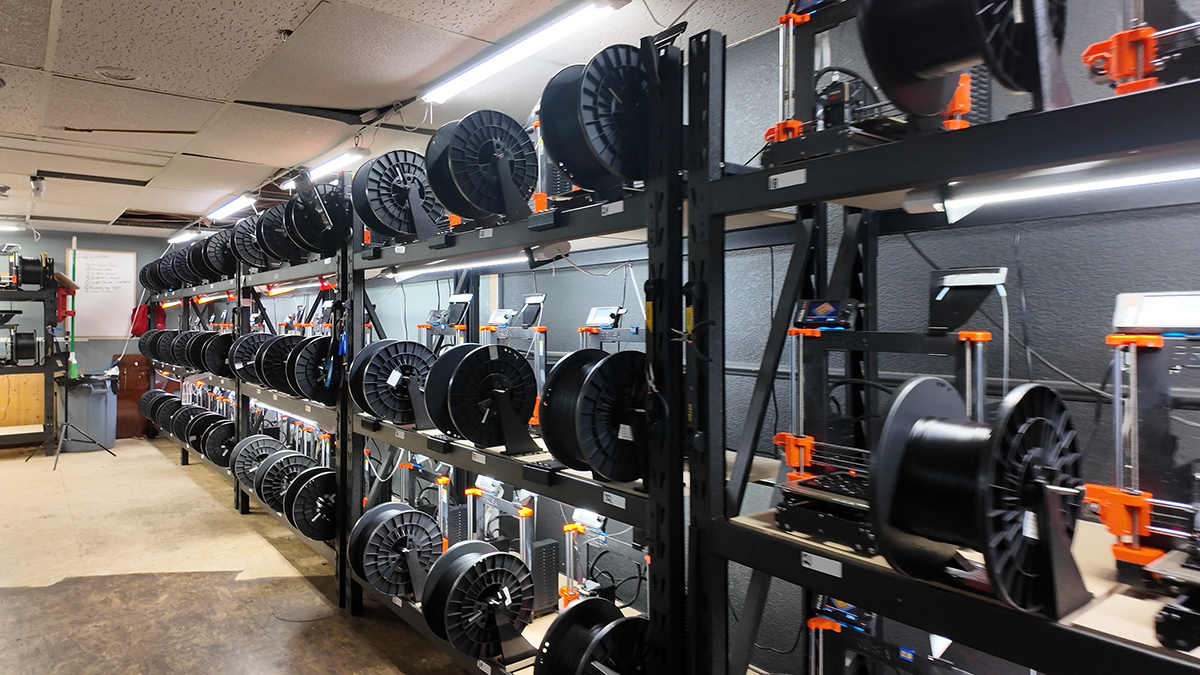
\includegraphics[width=\textwidth]{figures/images/literature/3dprintfarm.jpg}
    \caption{3D nyomtató farm}
\end{figure}

Egy ilyen farm esetén, már egy szeletelési hiba is, ha észrevétlen marad anyagi kárral, nyersanyagveszteséggel
vagy a berendezések sérülésével járhat.
A projekt keretein egy olyan skálázható rendszert szeretnénk megvalósítani, mely képes minden nyomtatón figyelni a darabokat, és
hiba kategóriának megfelelően jelezni amenyiben beavatkozásra van szükség. Az alapötlet: Egy olyan konvoluciós neuron háló
betanítása mely képes felismerni az alap hibákat, es ennek a beillesztése egy olyan keretrendszerbe, mely a nyomatott darabot több szemszögből figyeli.

\chapter{Irodalomkutatás}
\section{Bevezetés}

A 3D nyomtatási folyamatok automatizált hibadetekciójának kutatása az elmúlt évtizedben kiemelkedő
figyelmet kapott, különösen az additív gyártás ipari elterjedésével párhuzamosan. A szakirodalom
két fő megközelítési irányt különböztet meg: a \textbf{képalapú} (gépi látás és mélytanulás) és az
\textbf{akusztikai jelalapú} módszereket. Jelen fejezet áttekinti a terület legfontosabb publikációit,
különös tekintettel az FDM nyomtatókra, a valós idejű detekciós rendszerekre, valamint a
konvolúciós neurális hálózatok alkalmazására, amelyek a jelen projekt elméleti alapjait képezik.

% -------------------------------------------------------------------
\section{Képalapú megközelítések}

    \subsection{Klasszikus képfeldolgozás és referencia-alapú anomáliadedekció}

    A képalapú hibadedekció egyik úttörő megközelítése a referenciakép-összehasonlítás: a
    rendszer az élő kamerakép és egy ideális, hibamentes referencia közötti különbségeket keresi.
    Petsiuk és Pearce~\cite{petsiuk2021hog} nyílt forráskódú, rétegenkénti anomáliadetekciós
    rendszert fejlesztett ki, amelyben a referencia képeket nem valódi nyomtatásból, hanem
    G-kód alapján, Blender fizikai renderelőmotorral szintetikusan állítják elő. A detekció
    irányított gradiens hisztogramok (\textit{Histograms of Oriented Gradients}, HOG) hasonlóságának
    mérésén alapul. A módszer hat reprezentatív hibatípus, köztük a spagetti-jelenség, a
    réteg-eltolódás és az idegen tárgy jelenléte, azonosítására terjed ki, és különlegessége,
    hogy előzetes betanítási adathalmazt nem igényel. Tizenkét hasonlóság- és távolságmérték
    összehasonlítása alapján a Pearson-korreláció, a Spearman-féle rangkorreláció és a koszinusz-hasonlóság
    bizonyult a legmegbízhatóbbnak.

    Egy másik referencia-összehasonlításon alapuló megközelítést mutat be Ben Hammouda és
    társai~\cite{benhammouda2024defect} munkája, amelyben az FDM nyomtatás során keletkező hibákat
    képfeldolgozási technikák, él- és textúraanalízis, szegmentálás, segítségével azonosítják.
    A vizsgált módszerek az STL-fájlokból generált ideális képekkel vetik össze a valódi rétegfelvételeket,
    és különböző geometriai eltérések alapján adnak visszajelzést a nyomtatás minőségéről.
    A kísérletsorozat megerősíti, hogy a kétdimenziós összehasonlítás hatékonyan alkalmazható
    olyan makroszintű hibák felismerésére, mint a vetemedés vagy az alulextrúdálás, ám korlátai
    mutatkoznak finom, kis területre lokalizált defektusok esetén.

    \subsection{Mélytanulás alapú, valós idejű hibadedekció}

    A mélytanulási módszerek, különösen a konvolúciós neurális hálózatok (CNN), új lehetőségeket
    nyitottak a 3D nyomtatási hibák valós idejű, automatikus felismerésében.

    Paraskevoudis és társai~\cite{paraskevoudis2020stringing} egy mély konvolúciós neurális hálózatot
    fejlesztett ki kifejezetten a szálazás (\textit{stringing}) hibatípus felismerésére FFF
    nyomtatásoknál. A modellt élő videóbemenetről szerzett, szálazást ábrázoló képeken tanították be,
    és valós nyomtatási környezetben tesztelték. Az eredmények szerint a módszer nagy sebességgel
    és megbízható pontossággal azonosítja a hibát, és lehetőséget nyújt a folyamat automatikus
    megállítására vagy a nyomtatási paraméterek korrekciójára. A tanulmány hangsúlyozza, hogy
    a kameralapú detekció különösen hatékony azon hibatípusoknál, amelyek vizuálisan, a darab
    és folyamat megfigyelése alapján azonosíthatóak, szemben a forrástüneti hibákkal, amelyek
    érzékelőkkel közvetlenül is detektálhatók.

    Zhang és társai~\cite{zhang2023multiaxis} többtengelyes FDM nyomtatáshoz fejlesztett offline
    minőségellenőrző rendszert, amelyben egy CCD-kamera rögzíti az egyes rétegeket, a CNN pedig
    osztályozza a hibákat. Az interlayer stripping (rétegek közötti szétválás) tipikus defektus
    felismerésére validálták a módszert: az osztályozási pontosság 83,1\%, az érzékenység 85,6\%
    volt, a ROC-görbe alatti terület 0,824-et ért el, ami igazolja a módszer megvalósíthatóságát
    és terjeszthetőségét más hibatípusokra is.

    Átfogó áttekintést nyújt a területről Armin és társai~\cite{armin2025review} összefoglaló tanulmánya,
    amely rendszerezi a képfeldolgozás és gépi látás 3D nyomtatási hibadetekcióban alkalmazott
    módszereit. A szerzők külön tárgyalják a hagyományos, kézi jellemzőkinyerésen alapuló és a
    modern, végponttól végpontig automatizált mélytanulási megközelítéseket, valamint a
    teljes referenciás (\textit{full-reference}) és referencia nélküli (\textit{no-reference})
    módszereket. A review következtetése szerint a valós idejű monitorozó rendszerek fejlesztése
    az anyagveszteség csökkentésének és a fenntartható additív gyártásnak kulcseleme, a jövőbeli
    fejlesztések várhatóan az autonóm visszacsatolási mechanizmusok irányába mutatnak.

    \subsection{Háromdimenziós gépi látás}

    A kétdimenziós képalapú módszerek korlátait, különösen kis méretű, mélységi információt
    igénylő defektusok esetén, 3D gépi látással igyekeznek feloldani.

    Zhao és társai~\cite{zhao2023geometric} pontfelhő-alapú detekciós módszert dolgoztak ki 3D
    nyomtatott felületek hibáinak azonosítására. Az általuk javasolt MBH kulcspontdetektor és INRoPS
    jellemzőleíró kombináció először kivon potenciális hibarégiót, majd pontszomszédsági számítással
    precízen meghatározza a hiba alakját. A módszer robusztusabb és pontosabb a korábbi 2D-alapú
    megközelítéseknél, kiemelten kis méretű defektusok felismerésekor, ahol a kétdimenziós
    képelemzés a zaj által elfedett hibaterületeket tévesen minősíti.

% -------------------------------------------------------------------
\section{Akusztikai alapú megközelítések}

Az akusztikai emisszió (\textit{Acoustic Emission}, AE) analízise egy nem romboló vizsgálati módszer,
amelyet a gyártóipar számos területén alkalmaznak a strukturális épség monitorozásához. Az
additív gyártásban a nyomtatás közbeni anyagkölcsönhatások, repedésképződések és rétegkötési
problémák jellegzetes hangjelet keltenek, amelyek elemzéséből a hiba típusára és helyére
következtetni lehet.

Barriga-Machado és társai~\cite{barriga2025acoustic} PLA alapú, extrudálással előállított minták
károsodásmechanizmusait vizsgálták AE-analízissel kombinálva felügyelet nélküli (\textit{DBSCAN},
\textit{k-means}) és hibrid felügyeletes (\textit{CNN} spektrogram alapú) tanulási módszereket.
A DBSCAN két jól elkülöníthető klasztert azonosított: alacsony frekvenciás (0-260\,kHz) és magas
frekvenciás (270-390\,kHz) csoportot, amelyek a filament törési és a rétegközi szétválási
mechanizmusoknak felelnek meg. Az eredmények igazolják, hogy az adathajtott AE-analízis gyors és
nem romboló eszközt jelent az \textit{in-situ} károsodásdetekciókhoz polimer additív gyártásban.

Waheed és Bernadin~\cite{waheed2023acoustic} valós idejű hangjelalapú hibadetektáló rendszert
fejlesztett FDM nyomtatókhoz CNN-modell alkalmazásával. A rendszer a nyomtatás során keletkező
hangjeleket rögzíti és spektrogrammá alakítja, amelyeket a CNN oszt be hibatípus szerint.
A vizsgált hibakategóriák között szerepelt a fúvókadugulás, a filamentszakadás és a fogaskerék-csúszás.
A kontaktus nélküli, skálázható megközelítés, szemben a hagyományos érzékelőalapú megoldásokkal,
nem igényel közvetlen mechanikai integrációt a nyomtatóba, és az előzetes mérések alapján
megbízható valós idejű hibajelzést képes nyújtani.

Bin Zainal és társai~\cite{binzainal2025lpbf} lézeres porfúziós (\textit{Laser Powder Bed Fusion},
L-PBF) fémes additív gyártási folyamatban alkalmaztak akusztikus monitorozást. A mérőrendszer
mikrofonnal rögzítette az L-PBF folyamat során keletkező akusztikus jeleket, amelyekből hullámlet-transzformáció
(\textit{wavelet transform}) segítségével nyertek ki jellemzőket. Véletlenerdő (\textit{random forest})
és legközelebbi szomszéd (\textit{k-nearest neighbor}) osztályozókkal átlagosan 94\%-os
anyagjellemzési pontosságot értek el, igazolva az akusztikai módszer potenciálját a folyamatparaméterek
valós idejű ellenőrzéséhez.

% -------------------------------------------------------------------
\section{YOLO-alapú tárgydetekció ipari alkalmazásokban}

A YOLO (\textit{You Only Look Once}) objektumdetekciós modellek az iparban is egyre szélesebb
körben terjednek, köszönhetően kiemelkedő sebességüknek és pontosságuknak. Jóllehet az alábbi
tanulmány nem 3D nyomtatásra, hanem acélfelületek hibadetekciójára fókuszál, módszertanilag
szorosan kapcsolódik a jelen projektben alkalmazott megközelítéshez.

Wang és társai~\cite{wang2023yolov5steel} valós idejű acélfelület-hibadedekciós rendszert fejlesztett
többléptékű YOLOv5-alapon. A hálózathoz speciális többléptékű feltáró blokkot és térbeli figyelemfigyelmet
(\textit{spatial attention mechanism}) integráltak a különböző méretű felületi hibák hatékony
felismeréséhez. A NEU-DET adathalmazon elért ~72\%-os mAP érték és a valós idejű sebesség
igazolja, hogy a YOLO-architektúra gyári minőség-ellenőrzési feladatokra, a 3D nyomtatás
hibadetekciójához hasonló körülmények között, megbízhatóan alkalmazható. A többléptékű
megközelítés különösen fontos, mivel az additív gyártás hibái is rendkívül változatos méretekben
és megjelenési formákban fordulnak elő.

% -------------------------------------------------------------------
\section{Összefoglalás és a projekt kontextusa}

A fenti szakirodalom áttekintéséből több fontos következtetés vonható le.

Egyrészt, a \textbf{képalapú, mélytanulási módszerek}, különösen a YOLO-architektúrán alapuló
egymenetes detektorok, a valós idejű ipari hibadetekció legsikeresebb eszközei, amelyek a
referenciaalapú és hagyományos képfeldolgozásnál rugalmasabban generalizálnak, és nem igényelnek
előre meghatározott geometriai modellt.

Másrészt, az \textbf{akusztikai megközelítések} komplementer információt nyújtanak, különösen
belső (a kamerával nem látható) strukturális hibák esetén, azonban valós idejű FDM-alkalmazásokban
még korlátozott az elterjedtségük a szükséges szenzorintegráció és a zajszűrés nehézségei miatt.

Harmadrészt, az áttekintett megoldások többsége \textbf{egyetlen kameraállást} alkalmaz, ami
korlátozza a detektálható hibatípusok körét. Ezt a korlátot a jelen projekt egy
\textbf{többkamerás architektúrával} hivatott feloldani, lehetővé téve, hogy a nyomtató különböző
nézőpontjaiból érkező képek együttes feldolgozásával robusztusabb detekciós rendszer valósuljon meg.

A vonatkozó irodalom alapján a projekt a mélytanulás, konkrétan a YOLOv8, és a valós idejű
kamerastreaming kombinációjára épít, igazodva a terület tudományos konszenzusához, miközben az
általánosabb ipari alkalmazhatóságot és skálázhatóságot is szem előtt tartja.


\chapter{Elméleti háttér}
\section{3D nyomtatásról TODO!}

    A 3D nyomtatás maga egy olyan addítív gyártási folyamat mely CAD vagy digitális 3D modellt épít fel
    különböző nyersagokat felhasználva, 3D nyomtatók segítségével. Ma a két legelterjetteb 3D nyomtató
    típus az SLA, mely különleges erre a célra alkalmas gyanta és UV sugarak segítségével építi fel a darabot,
    és az FDM nyomtatók melyek különböző műanyagból készült filamentet használnak nyersanyag gyanánt.
    Mindkét típus bár teljesen más elven működik rétegenként építi fel a darabot egy előre szeletelt
    G-kód-ot követve. A dolgozat általi megvalósítás FDM tipűsú nyomtatókkal foglalkozik.\\ 

    \begin{figure}[H]
        \centering
        \begin{minipage}[t]{0.48\textwidth}
            \centering
            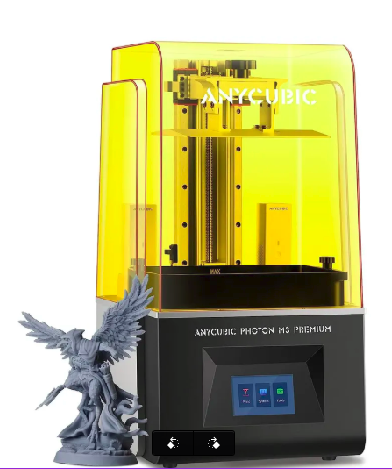
\includegraphics[width=\linewidth,height=6cm,keepaspectratio]{figures/images/literature/SLA.png}
            \caption{SLA nyomtató}
        \end{minipage}\hfill
        \begin{minipage}[t]{0.48\textwidth}
            \centering
            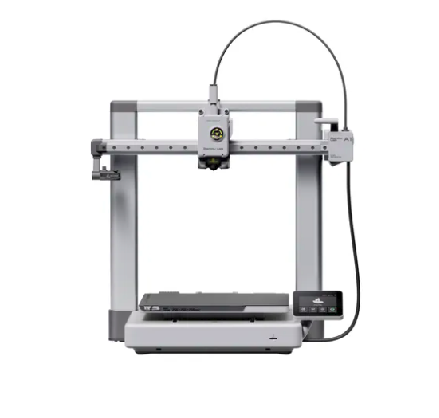
\includegraphics[width=\linewidth,height=6cm,keepaspectratio]{figures/images/literature/FDM.png}
            \caption{FDM nyomtató}
        \end{minipage}
    \end{figure}

    Mint már említettem az FDM 3D nyomtatók különböző filamenteket használnak nyersanyagként, 
    ezekből is több fajta létezik. A legismertebb ezek közül a PLA, mellyel könnyű jól dolgozni,
    főként prototípusok és dísztárgyak nyomtatására alkalmazzuk, mivel az anyag fő gyengesége
    az alacsony olvadáspont (körülbelül 70 celzius fok), és az UV sugarak és a nedvesség és hamar
    kikezdik. Ismertebb filament típusok még a PETG mely jobb mechanikai tulajdonságokkal és ellenálló
    képességgel rendelkezik de még mindig nem az igazi, ha teljes mértékben szükség van mindennemű mechanikai
    ellenállásra, terhelhetőségre akkor ABS-t kell nyomtatnunk, ennek nyomtatása viszont igen igényes, mivel zárt
    teret és állandó hőmérsékletet igényel.Amennyiben pedig flexibilis tárgyakat nyomtatnánk a TPU a mi megoldásunk.


    \begin{figure}[H]
        \centering
        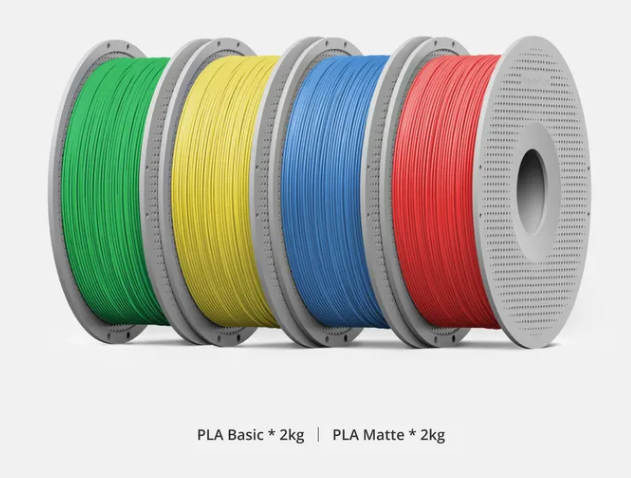
\includegraphics[width=0.6\textwidth]{figures/images/literature/filament.png}
        \caption{Filament tekercsek}
    \end{figure}

        \subsection{Felmerülő hibák és limitációk}
        A 3D nyomtatási folyamat során rengeteg hiba felmerülhet. mely több okból is keletkezhet,
        a nedves anyagtól, a rossz kallibrációig, vagy akár komoly hardver hibáig is. Beszéljünk
        egy kicsit ezen hibákról.

            \subsubsection{Stringing- Avagy szálazás}
                
                \begin{figure}[H]
                    \centering
                    \rotatebox{270}{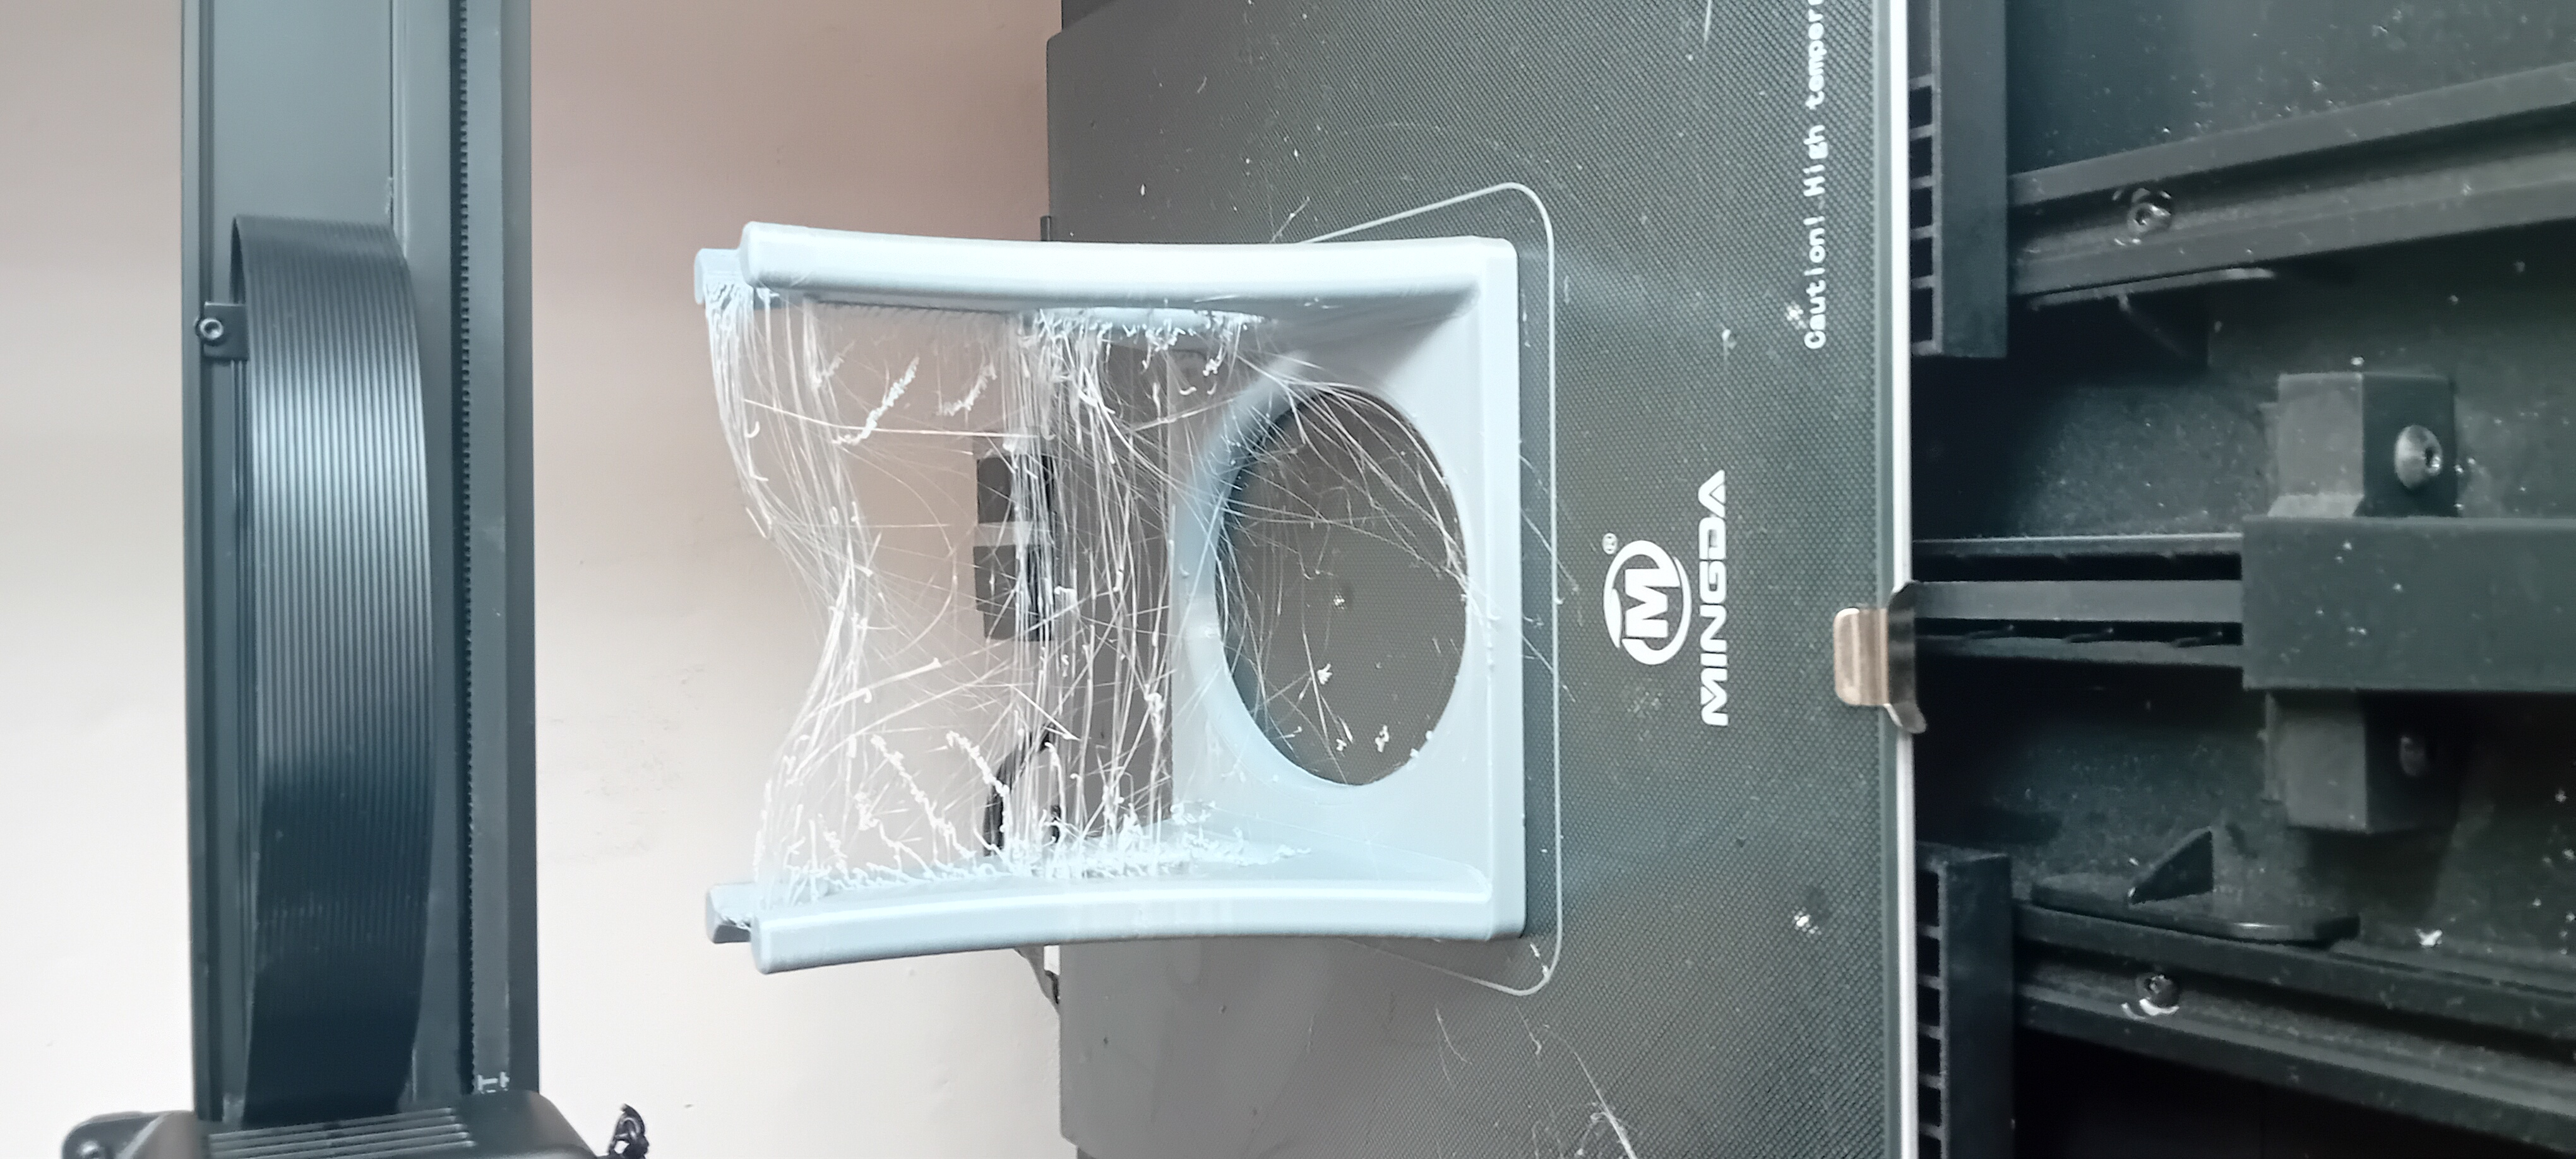
\includegraphics[width=0.6\textwidth]{figures/images/literature/string.jpg}}
                    \caption{Szálazás a nyomtatás végén}
                \end{figure}

            Ez a hiba igen idegesítő tud lenni, mivel rengeteg utómunkát igényel a vékony szálacskák
            eltávolítása, és még úgyis megmarad a nyoma. Több előokozó tényező is lehet. Szeletelés
            során nem megfelelő visszahúzás beállítási érték, nedves filament, túl nagy fúvóka hőmérséklet 
            vagy mocskos fúvóka.


            \subsubsection{Warping- Avagy eltorzulás}

                \begin{figure}[H]
                    \centering
                    {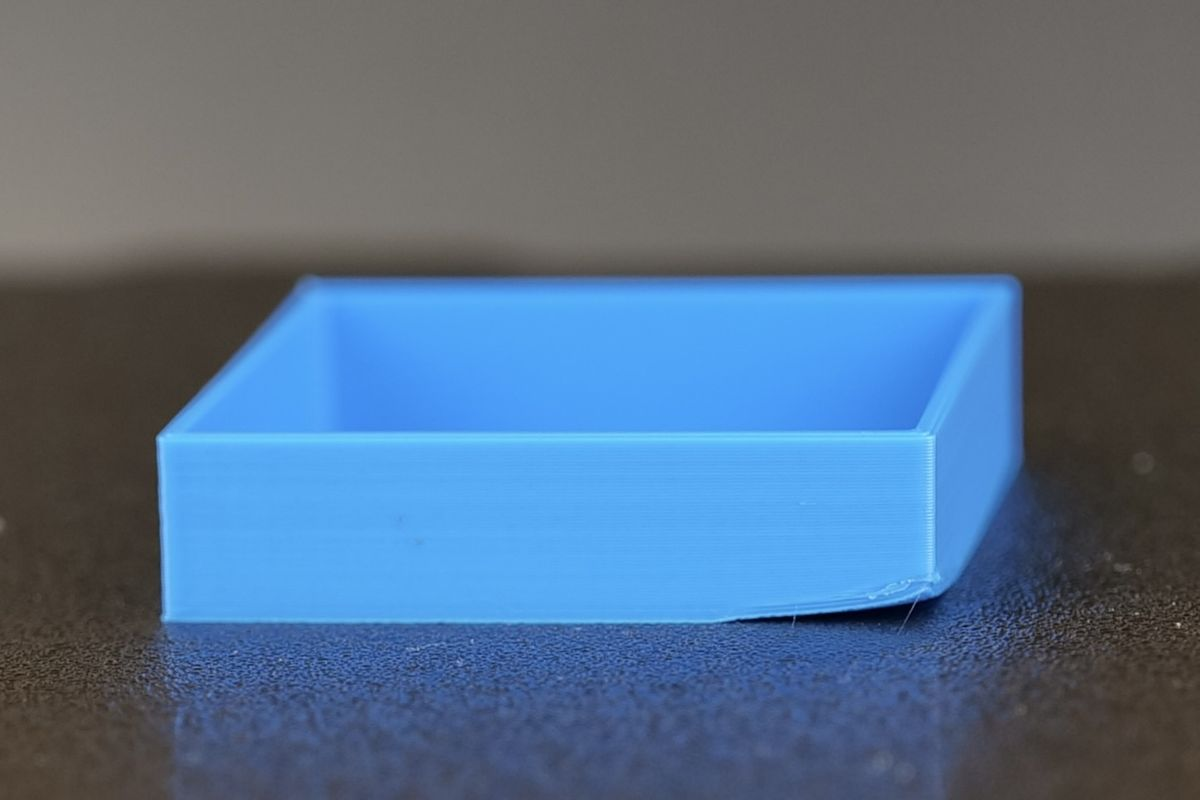
\includegraphics[width=0.6\textwidth]{figures/images/literature/curling_corner.jpg}}
                    \caption{Eltorzult darab}
                \end{figure}

            Eltorzulás legtöbbször akkor jelentkezik, amikor egy darab alján éles szögek találhatóak, 
            például négyzet, vagy egyébb sokszög. Fontos beavatkozó viszont a tárgyasztal hője, tisztasága
            is a megfelelő tapadás fenttartásához. A hiba maga kiküszöbőlhető egy úgynevezett skirt, 
            avagy szoknya alkalmazásával a szeletelőben, mely búnusz tapadást biztosít a sarkakon.

            \subsubsection{Layer shift-Avagy réteg eltolódás}

                \begin{figure}[H]
                    \centering
                    {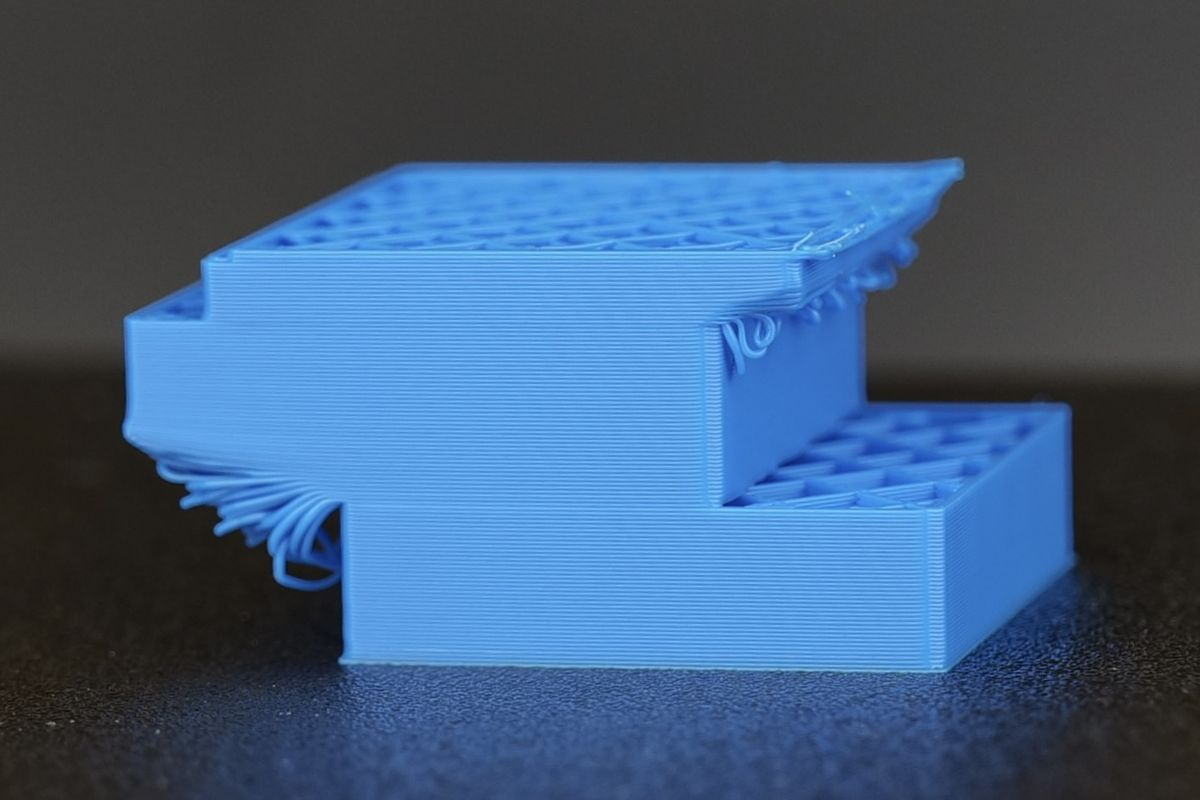
\includegraphics[width=0.6\textwidth]{figures/images/literature/layer_shifts.jpg}}
                    \caption{Elcsúszott rétegek}
                \end{figure}

            A nyomtatott rétegek eltolódása végzetes hiba a darab számára. Főként akkor jelenik meg amikor 
            eltérés van a G-kódban található koordítnáta és a fúvóka világi koordínátái között. Három fő oka
            van, túl nagy nyomtatási sebesség, nem megfelelő Z-offset mely miatt a fúvóka beleakadhat a darabba
            ezzel koordínáta különbséget előídézve, vagy a nyomtatót ért fizikai trauma, esetleg laza sínek 
            vagy merevítők.

            \subsubsection{Under extrusion- Avagy alul extrúdálás}

                \begin{figure}[H]
                    \centering
                    \begin{minipage}[t]{0.48\textwidth}
                        \centering
                        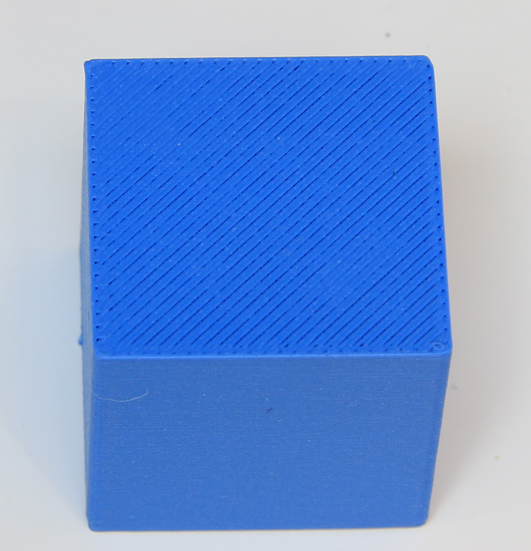
\includegraphics[width=\linewidth,height=6cm,keepaspectratio]{figures/images/literature/underex.png}
                        \caption{Teljes alul extrúdálás}
                    \end{minipage}\hfill
                    \begin{minipage}[t]{0.48\textwidth}
                        \centering
                        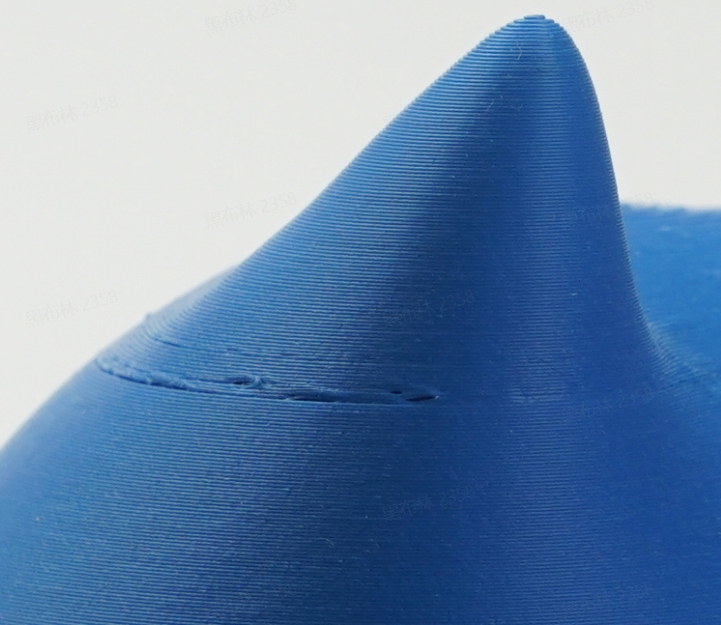
\includegraphics[width=\linewidth,height=6cm,keepaspectratio]{figures/images/literature/lokunderex.jpg}
                        \caption{Lokális alul extrúdálás}
                    \end{minipage}
                \end{figure}
    
            Ezen hibának két külön fajtáját különböztetjük meg, a teljes illetve a lokális alul extrúdálást.
            Ezen hiba okai lehetnek mind hardveres, de előokozhatja nem megfelelő szeletelés is. 
            Főbb előidéző okok közé tartozik, hogyha, eldugul a ptfe cső, vagy idegen test kerül bele, beakadt
            a filament tekercs és nem jút elég a fúvókához, fogaskerék probléma, vagy részleges dugúlás a fúvókában 
            vagy a hotendben. Amennyiben a problémát szoftveres ok váltja ki a Maximum Volumetric speed illetve Flow
            ratio nevű beállításokkal van a probléma. A mai modern nyomtatók már fel vannak szerelve autómatikus adagolás
            kallibrációval, ezzel segítve a felhasználót.

            \subsubsection{Over extrusion- Avagy felül extrúdálás}

                \begin{figure}[H]
                    \centering
                    {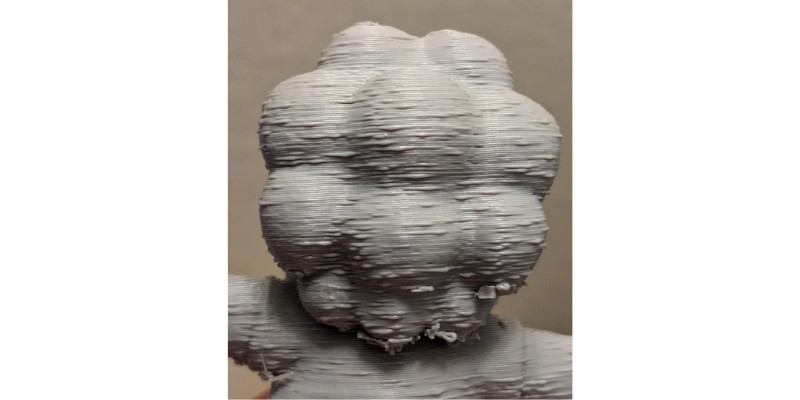
\includegraphics[width=0.6\textwidth]{figures/images/literature/overex.jpg}}
                    \caption{Felül extrúdált darab}
                \end{figure}

            Ugyanazon probléma mint az alul extrúdálás, egy annyi csavarral, hogy itt nem túl kevés anyag jut a 
            fúvókához hanem pont, hogy túl sok.

            \subsubsection{Nozzle Clog- Avagy fúvóka dugulás}

                \begin{figure}[H]
                    \centering
                    {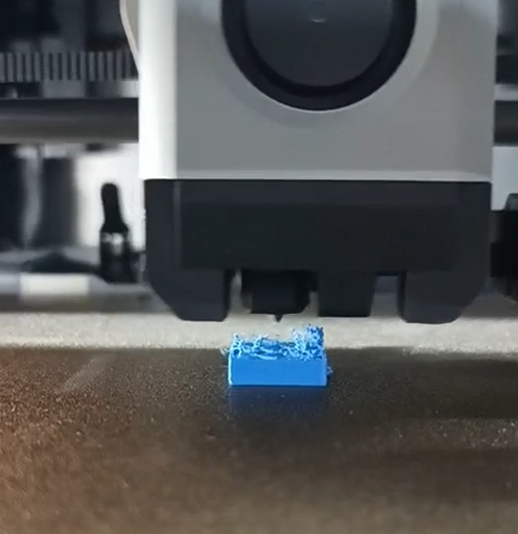
\includegraphics[width=0.6\textwidth]{figures/images/literature/clog.png}}
                    \caption{Nyomtatás közben eldugult fúvóka és darab}
                \end{figure}

            Egy sajnos igen gyakori probléma mely akár a nyomtatónk "életébe" is kerülhet. Legfőbb oka, hogy 
            a filament amikor a ptfe csövön keresztül a forró kamrába, majd pedig a fúvókába jut nem teljesen 
            tiszta, kis por vagy egyébb szennyező anyagok is bekerülnek, melyek a fúvóka dugulását okozhatják. 
            Amennyiben nem vesszük észre hamar az olvadt műanyag felgyülhet a fúvókában és belülről szétfeszíti azt, 
            ezzel jelentős anyagi kárt okozva.

            \subsubsection{Foreign object on the printbed- Avagy idegen tárgy a tárgyasztaklon}

            Ezen hiba se nem hardveres se nem szoftveres hanem szimplán a kezelő figyelmetlensége miatt 
            következik be, akik a tapasztalatomból legtöbbször olyan izgatott a szeletelést követően, 
            hogy elfelejti ellenőrizni, hogy leürítette-e a tárgyasztalt, vagy csak karbantartás után 
            nem pakolt el maga után. Az idegen tárgyak a fúvókában és a fejben súlyos anyagi kárt okozhatnak 
            viszont, hiszen a legtöbb nyomtató nem képes detektálni, ha a tárgyasztal üres vagy sem.
                
                \begin{figure}[H]
                    \centering
                    {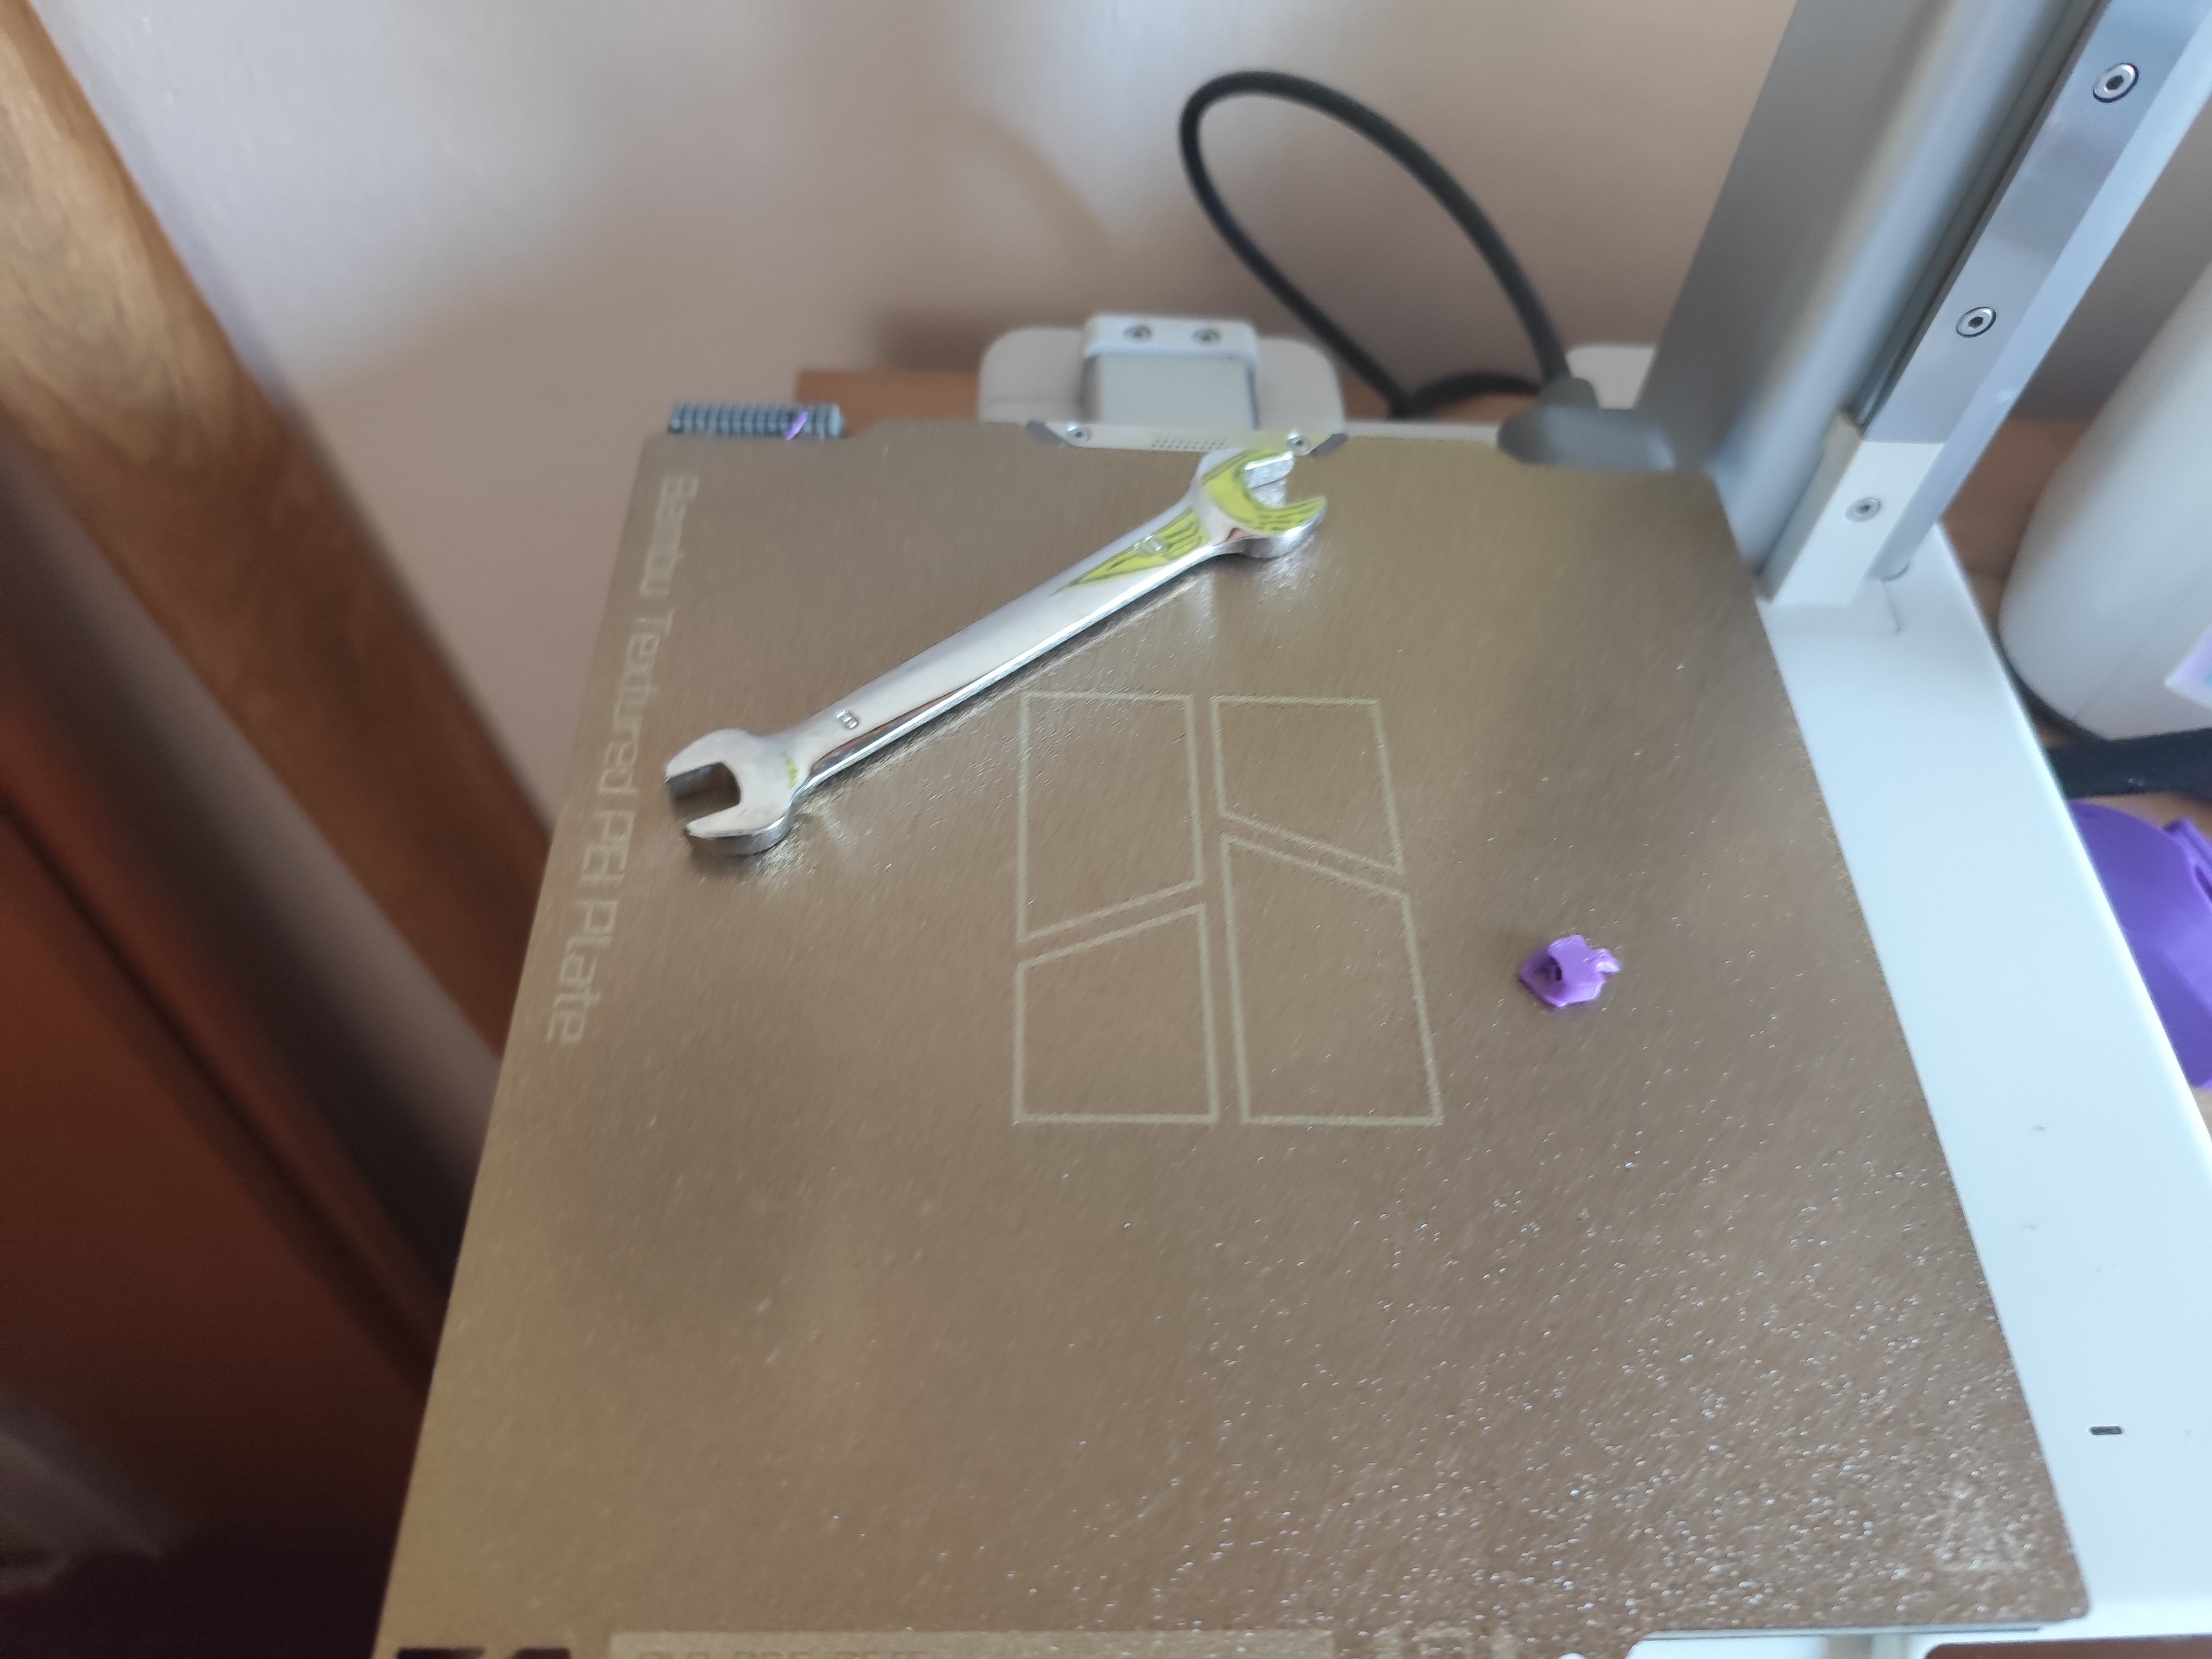
\includegraphics[width=0.6\textwidth]{figures/images/literature/foreign.jpg}}
                    \caption{Figyelmetlenségből a tárgyasztalon hagyott szerszám}
                \end{figure}

            \subsubsection{First layer not sticking- Avagy az első réteg nem tapad}

                \begin{figure}[H]
                    \centering
                    {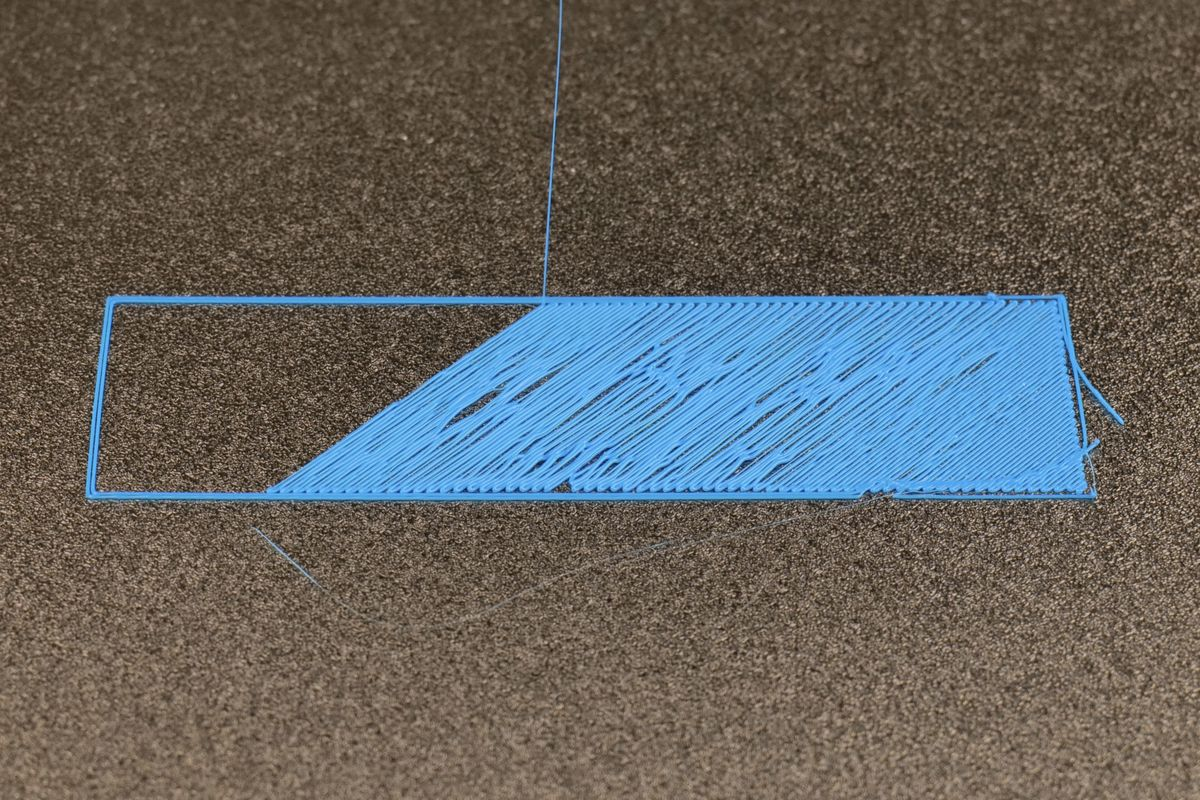
\includegraphics[width=0.6\textwidth]{figures/images/literature/first_layer_not_sticking_to_the_plate.jpg}}
                    \caption{Nem tapadó első réteg}
                \end{figure}

            A 3D nyomtatási folyamat során a legfontosabb mozzanat az első réteg, ha ez nem tapad 
            oda akkor az egész darab kuka, fontos figyelemmel kísérni, amennyiben észrevétlen marad, 
            az Spagettihez, és rengeteg anyag veszteséggel jár. Főbb okai, ha a tárgyasztal nem megfelelő 
            tisztaságú, rossz fúvóka tárgyasztal távolság (Z-offset), vagy rossz asztal szintezés. Könnnyen 
            elkerülhető a megfelelő beállításokkal és a tárgyasztal karban-és tisztán tartásával.

            \subsubsection{Spagetti- Avagy az anyag a levegőbe adagolódik}

            Rengeteg oka lehet, de a legfőbb előokozója, ha az első réteg nyomtatási folyamata sikertelennek 
            bizonyult, a fúvókát ez nem érdekli, ő követi a G-kód által megadott utasításokat és addig nyomja a 
            levegőbe az anyagot, ameddig a végére nem ér, vagy a kezelő azt meg nem állítja. 
            Fontos kiemelni, hogy a tapadás elvesztése a nyomtatási folyamat bármely pillanatában bekövetkezhet, 
            amennyiben nem megfelelő support beállításokat alkamaztunk a szeletelőben, vagy éppen a supportok 
            engedik el a tárgyasztalt, ezzel védtelenül hagyva a darabot.

                \begin{figure}[H]
                    \centering
                    \rotatebox{270}{
\includegraphics[width=0.6\textwidth]{figures/images/literature/spagetti.jpg}}
                    \caption{Hibás nyomtatást követő spagetti halmaz}
                \end{figure}



\chapter{Mélytanulási modellek}
    \section{Piackutatás és a megfelelő Ai modell kiválasztása}

        \subsection{Lehetséges eszközök}

        Képfelismerésre, több ai keretrendszer felhasználható, már nem kell abban gondolkozni, hogyha megszeretnénk valósítani valamit akkor fel kell építenünk
        egy egész neuron hálót a semmiből, viszont fontos, hogy olyat válasszunk mely számunkra a legmefelelőbb a cél megvalósításhoz. Amikor a projekt körvonalazódott
        a fejemben, az ultralytics yolov5 gondolata jelent meg mivel már dolgoztam vele, az egyetemi Mesterséges Intelligencia tantárgy során tudom, mire képes.
        De azért további utána olvasás során rá kellett jönnöm, hogy nem feltétlen ez a legjárhatóbb út, vannak jobb megoldások. Egy nagyon fontos szempont volt
        a választásban, hogy a tanított modell könnyen integrálható legyen egy olyan pipeline-ba mely nagyban kapaszkodik a Jupyter Notebook, majd később a Google Cloud által kínált erőforrásokba,
        ezzel megkerülve a tanítás és futtatás során felmerülő hardverbéli megszorításokat.

        \subsubsection{Faster R-CNN}
        A Faster R-CNN, azaz régió alapú konvolúciós neuron háló, úgynevezett kétfázisú obiektum észlelő neurális háló. Megjelenése 2015-re
        vezethető vissza a Microsoft Research kutatói rukkoltak elő vele. Működési elve röviden három lépésre bontható. Először végbemegy 
        a jellemző kivonás, mely során egy előre betanított konvoluciós háló vizuális jellemzőtérképet készít a bebementi képből. Ezt követi a 
        Region Proposal network felépítése, ezen folyamat során generálódnak ki a lehetségers jelöltek, jelentősen gyorsabb mint a manuális régió 
        kereső algoritmusok.A harmadik egyben utolsó lépcsőfok a Rol pooling és az osztályozás, ebben a jellemző térképből kivágódnak a javasolt régiók, 
        majd egységes méretre skálázás történik, ez a Rol pooling. Végezetül egy másodlagos hálózat minden régiót egyenként kiértékel, és megmutatja melyik 
        régió melyik obiektumhoz társul majd egyben pontosítja a határoló doboz koordinátáit.
        A Faster R-CNN modell előnyei, a magas pontosság, melyet a kétfázisu feldolgozásnak köszönhet. Az előre betanított konvulicós háló nagyon rugalmas, 
        és könnyen összehangolható más konvoluciós neuron hálókkal, ezáltal a háló teljesítménye skálázható.
        Hátrányai miatt számunkra rossz alternatívává válik, hiszen lassú interferenciája miatt, nem képes valósidejű alkalmazások megvalósítására. A modell 
        mérete is szintén elég nagy mely erős hardverigényt jelent. Integrálása a Jupyter Notebook-ba is sokkal elvontabb mint például a Yolo család tagjaié.

        \subsubsection{Yolov5}
        A Yolov5 avagy You Only Look Once 5ös verziója, egy egyfázisű objektumdetekciós neurális hálózat. 2020-ban adta ki az Ultralytics nevű cég. 
        Eléggé széleskörben elterjedt az iparban mivel, nagyon könnyen használható, és tanítható, és nagyon könnyen integrálható. A Yolo Architektúra is h
        árom részből épül fel. Az első a Gerinc mely a képből kinyeri a vizuális jellemzőket, majd a Yolov5 a Cross Stage partial Darknet elvégzi a számításokat. 
        Ez a réteg felel az összes vizuális mintázat felismeréséért, melyből később majd a háló tanulni fog. Az architecktúra 
        második része a nyak, mely először összevonja a különböző méretű jellemzőket, biztosítva hogy a modell több méretű obiektum felismerésére
        is képes legyen. A harmadik rész a fej, ezen rétegben történik a felismerés, ez egy horgony alapű réteg, a háló előredefiniált méretű dobozat
        próbál végig. Maga a kimenet három méretben jön létre.
        Előnyei közül kiemelendő, hogy kis interferencia ideje van, ezáltal tökéletes a valós idejű felismerésre modellmérettől függően. 
        Nagyon könnyen tanítható és integrálható, szinte out of the box használható. Jól dokumentált és rengeteg segédanyag található az interneten, 
        és a Hyperparaméterek augmentációk és a veszteség függvények is előre bevannak már állítva. A yolov5 egy jó kandidátus a projektünk szempontjából, 
        de újabb variánsa a Yolov8 még az ő hiányosságain is felülkerekedik, mivel a teljes Architektúrát újragondolták,ő jobb pontosságot és sebességet kínál, 
        és a detekció sem horgony alapű már.

    \section{A projekt megvalósításához használandó AI modell- YOLOv8}
    
    \subsection{Bevezetés}
        A YOLOv8 (\textit{You Only Look Once},8-as verziója)-at az ultralytics cég adta ki 2023-ban. Egy olyan modell, mely rendkívűl hasznos a valósidejű 
        obiektumdetektációban, emiatt is esett rá a választás, minden karakterisztikája megfelelő, ha 3D nyomtatási folyamatot szeretnék felügyelni, és az 
        esetlegesen felmerülő hibákat észrevenni esetleg közbelépni. De mégis mi mi teszi a YOLOv8-at az általunk felhasznált csodafegyverré?
    
    
    \subsection{Főbb karakterisztikák}
    \begin{itemize}
        \item Az ulralytics teljesen újragondolta a modell architektúráját, a Pytorch helyett teljesen saját architektúrára való áttérés történt, 
        ez pedig visszafele inkompatibilitást jelent a YOLOv5 irányába.
        \item Támogat obiektum detekciót, szegmentálást, pozíció becslést, obiektum osztályozást és követést.
        \item A tanítás és a futtatás is egyaránt API-n és CLI-n keresztül történik, nincs szükség scriptekre.
        \item Exportálási lehetőségek olyan formátumokba mint az ONNX, CoreML és TensorRT
        \item Könnyen tanítható saját adathalmazokkal is.
    \end{itemize}
    
    Ezekből is látszik, hogy miért esett ezen modelre a választás. Az adathalmaz elkészült, a cimkézés megtörtént, a következő lépés egyértelműen 
    a tanítás lesz.
    
    
    \subsection{Modell variánsok}
    Felhasználási célok és hardverigény szerint a YOLOv8 több méretben elérhető, hogy több felhasználást legyen képes kiszolgálni.
    
    \begin{itemize}
        \item \texttt{yolov8n} – Nano- a legkisebb modell, nagyon gyors és alacsony hardverigényű
        \item \texttt{yolov8s} – Small
        \item \texttt{yolov8m} – Medium
        \item \texttt{yolov8l} – Large
        \item \texttt{yolov8x} – Extra large- Legnagyobb elérhető pontosság, viszont a legnagyobb hardverigényű is.
    \end{itemize}
    
    
    \subsection{Telepítési útmutató és alapszíntű felhasználás}
    
    Telepítés:
    \begin{verbatim}
    pip install ultralytics
    \end{verbatim}
    
    Alap példa képfeldolgozásra:
    \begin{verbatim}
    from ultralytics import YOLO
    model = YOLO("yolov8n.pt")
    results = model("mütyür.jpg")
    results.show()
    \end{verbatim}
    
    Mi a felhasználáshoz, azt szeretnénk, hogy egy python scripten keresztül a modell, valósidejű kameraképen fusson és deketáljon hibákat.
    
    \subsection{Saját dataset felhasználása tanításhoz}
    
    Mint már említettem a modell tanítható saját adathalmaz segítségével is, amennyiben az megfelelően fel lett címkézve és az exportált annotációk 
    formátuma is Yolo kompatibilis. Ahhoz, hogy ez lehetséges legyen egy \texttt{data.yaml} fájlra lesz szükségünk, mely minden fontos információt tartalmaz.
    Tanítási és Validációs adathalmazok helye, osztályok számossága és elnevezése.
    
    \begin{lstlisting}
    train: images/train
    val: images/val
    nc: 9
    names: ['stringing', 'warping', 'layer_shift', 'under_extrusion',
            'over_extrusion', 'nozzle_clog', 'foreign_object_on_print_area',
            'not_sticking', 'spagetti']
    \end{lstlisting}
    
    Tanítási folyamat elstartolása parancssoron keresztül:
    
    \begin{verbatim}
    yolo task=detect mode=train model=yolov8n.pt data=data.yaml epochs=50 imgsz=640
    \end{verbatim}
    
    \subsection{Annotáció formátuma}
    
    YOLO-formátumban minden kép mellé tartozik egy azonos nevű .txt file melynek tartalma a következőképpen 
    néz ki, minden sor egy obiektum, egy .txt file pedig több obiektumot is tartalmazhat:
    
    \begin{verbatim}
    <class_id> <x_center> <y_center> <width> <height>
    \end{verbatim}
    
    Az obiektumokat leíró értéket lebegőpontos ábrázolás módban vannak, kifejezve, egyenként a képpel arányosan 0-1 közötti értékekre 
    normalizálva. Az annotáláshoz CVAT szoftvert használtam.
        
    \begin{table}[h!]
    \centering
    \caption{YOLOv8 előnyei és hátrányai a projekt szempontjából}
    \label{tab:yolo_elonyok_hatranyok}
    \renewcommand{\arraystretch}{1.4}
    \begin{tabular}{|p{0.45\textwidth}|p{0.45\textwidth}|}
        \hline
        \textbf{Előnyök} & \textbf{Hátrányok} \\
        \hline
        Valós idejű objektumdetektálás & Nagy modellek (pl. YOLOv8x) jelentős GPU erőforrást igényelnek \\
        \hline
        Egyszerű és megismételhető tanítási folyamat & Kis adathalmazon hajlamos túltanulásra \\
        \hline
        Kis modellek is magas pontosságot érnek el & Zsúfolt vagy részben takart objektumok detektálása nehézkes \\
        \hline
        Docker konténerizációs támogatás & Valós idejű feldolgozás hálózati késleltetéstől függhet \\
        \hline
        Aktív közösség és folyamatos fejlesztés & Egyedi osztályokhoz saját adathalmaz gyűjtése szükséges \\
        \hline
    \end{tabular}
    \end{table}






\chapter{Hardver- és szoftverkörnyezet}
\section{A teljes rendszer}
        A rendszer egy edge–cloud hibrid architektúrára épül, amelynek két fő pillére van: egy helyszínen elhelyezett Raspberry Pi edge eszköz,
        valamint a Google Cloud Platform felhőinfrastruktúrája. A Pi feladata a kamerás képrögzítés és az adatok előfeldolgozása,
        míg a felhő végzi a gépi tanulás alapú hibadetekciót, az adattárolást és a felhasználói értesítéseket.
        Az adatfolyam iránya: Raspberry Pi → Pub/Sub (\texttt{frames-in}) → Dispatcher Cloud Function → Vertex AI végpont (YOLO inferencia)
        → Pub/Sub (\texttt{detections-out}) → Alert-Manager Cloud Function → Firestore + e-mail értesítés → Dashboard.
        A teljes rendszer architektúráját a \ref{fig:systemarch}. ábra szemlélteti.

                \begin{figure}[H]
                    \centering
                    {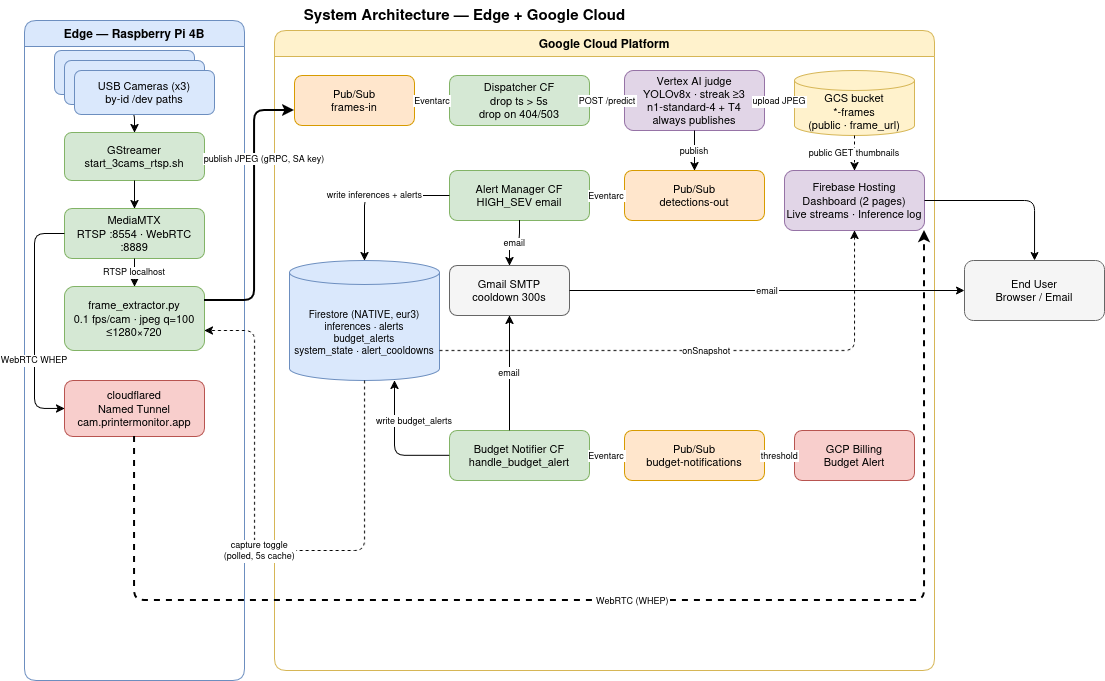
\includegraphics[width=\textwidth]{figures/images/literature/gcp_architecture.drawio.png}}
                    \caption{A rendszer}
                    \label{fig:systemarch}
                \end{figure}


\subsection{Kamera Agent – Raspberry Pi}
    A kamera képek előállításért felelő kamera Agent szerepét egy Raspberry Pi 4B 8GB tölti be,\cite{raspberry_pi}
    3 darab rácsatolt webkamerával kiegészítve. A Raspberry Pi mint edge eszköz rendkívül sokoldalú eszköz.
    Keveset is fogyaszt, megfelelő számú USB porttal is rendelkezik, és az erőforrások is megfelelőek számunkra.
    A Raspberry OS pedig tökéletes a szükséges Docker konténerek és Python szkriptek futtatására.
    


    \section{Szolgáltatások a Pi-n}
    A Pi-n három szolgáltatás fut, melyek az indítás után azonnal elindulnak systemd szolgáltatásként.
    Ezek nélkül a rendszer nem valósulhatna meg.

        \subsection{MediaMTX}
        A MediaMTX (korábban rtsp-simple-server) egy könnyűsúlyú, nyílt forráskódú médiaközvetítő szerver, mely Go programozási nyelven íródott\cite{mediamtx}.
        Szerepe a rendszerben, hogy a webkamerák által előállított nyers videófolyamokat RTSP protokoll szerint tegye elérhetővé a hálózaton.
        A Pi-n systemd szolgáltatásként fut, így az eszköz indításakor automatikusan elindul, emberi beavatkozás nélkül.
        Konfigurációs fájlja definiálja a három kamerastream elérési útját, a kódolási paramétereket, valamint az újracsatlakozási logikát.
        A H264-es kódolású RTSP végpontokat a Cloudflare alagúton keresztül éri el a dashboard, ahol WebRTC formátumban kerülnek megjelenítésre.
        A stream pipeline teljes folyamatát a \ref{fig:mediamtx}. ábra szemlélteti.

        \begin{figure}[H]
            \centering
            {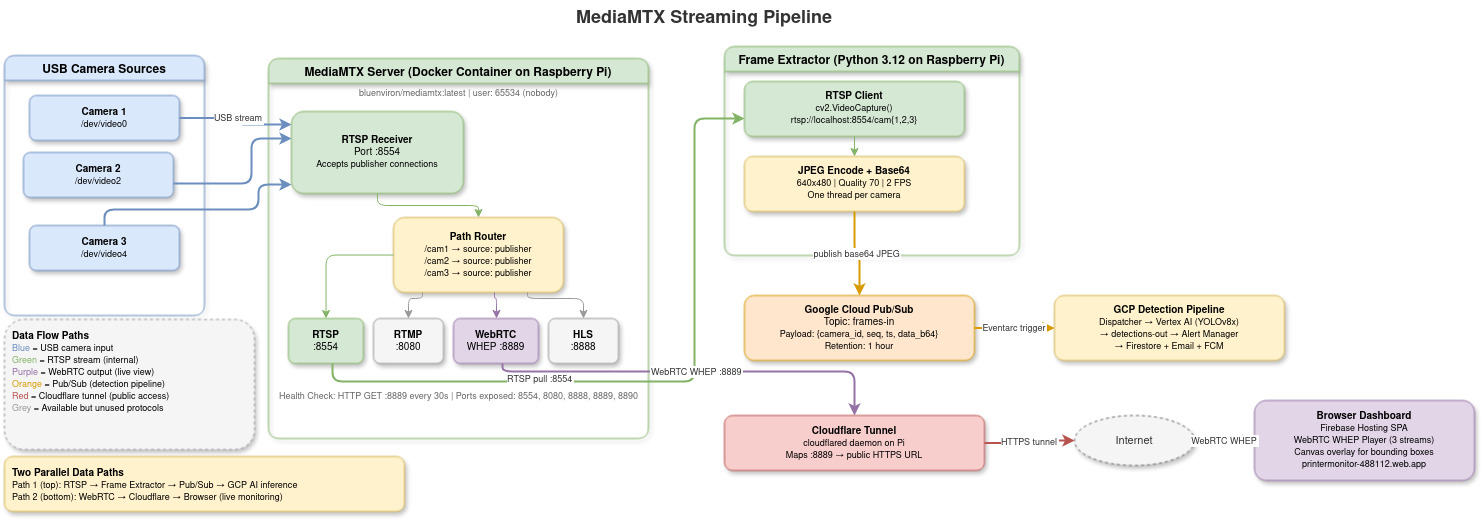
\includegraphics[width=\textwidth]{figures/images/literature/mediamtx_pipeline.jpg}}
            \caption{MediaMTX stream pipeline}
            \label{fig:mediamtx}
        \end{figure}

        \subsection{Képkockák kinyerése}
        A képkockák kinyerésért a \texttt{frame-extractor} szolgáltatás felelős, melynek belépési pontja a \texttt{main.py} Python script.
        Feladata, hogy a három RTSP streamből folyamatosan képkockákat olvasson ki, azokat feldolgozza, majd JSON üzenetként publikálja
        a \texttt{frames-in} Pub/Sub csatornára, ahonnan a \texttt{dispatcher} Cloud Függvény továbbítja őket a Vertex AI végpontra.
        A szolgáltatás a Pi-n systemd szolgáltatásként fut, és az \texttt{sa-frame-extractor} szervízfelhasználó kulcsával hitelesíti magát a Google Cloud felé.

        \subsubsection{Szálkezelés és olvasási modell}
        A script induláskor beolvassa a kamerák RTSP URL-jeit és azonosítóit a környezeti változókból. Minden kamerához két szál tartozik.
        Az első egy folyamatosan futó olvasószál (\texttt{FrameReader}), amely az OpenCV\cite{opencv} \texttt{VideoCapture} osztályán keresztül
        kapcsolódik az adott RTSP streamhez, és a beérkező képkockák közül mindig csak a legfrissebbet tartja meg, a hozzá tartozó,
        a beolvasás pillanatában rögzített UTC-időbélyeggel együtt. Így a publikált képkocka időbélyege a valós rögzítési időpontot tükrözi,
        nem pedig a feldolgozás idejét, ami elengedhetetlen a felhő oldalán végzett elavultság-szűréshez. Ha a kapcsolat megszakad, például
        a kamera újraindul vagy a hálózat elvész, az olvasószál automatikusan újracsatlakozást kísérel meg, így a rendszer emberi beavatkozás nélkül helyreáll.

        \subsubsection{Képfeldolgozás és publikálás}
        A kamerákhoz tartozó második szál a publikáló ciklus (\texttt{publish\_loop}), amely \texttt{CAPTURE\_FPS} ütemben
        (alapértelmezetten 0,1 fps, azaz kameránként tíz másodpercenként egy képkocka) kiveszi az olvasószáltól a legfrissebb képkockát,
        és elvégzi rajta a következő feldolgozási lépéseket:
        \begin{enumerate}
            \item Amennyiben a képkocka mérete meghaladja a konfigurált \texttt{FRAME\_WIDTH} × \texttt{FRAME\_HEIGHT} értéket (alapértelmezetten 1280×720 pixel),
                  az OpenCV a képarány megtartásával lekicsinyíti azt; a célméretnél kisebb képeket változatlanul hagyja.
            \item A képkocka JPEG formátumba kerül kódolásra a beállított \texttt{JPEG\_QUALITY} értékkel (alapértelmezetten 100).
            \item A JPEG bájttömb Base64 kódolással ASCII szöveggé alakul, hogy JSON üzenetbe ágyazható legyen.
            \item A script egy JSON objektumot állít össze, amely tartalmazza a \texttt{camera\_id} azonosítót, a \texttt{seq} szekvenciaszámot,
                  az \texttt{ts} UTC-időbélyeget, valamint a \texttt{data\_b64} mezőt a Base64-kódolt képpel.
            \item A kész JSON payload publikálásra kerül a Pub/Sub \texttt{frames-in} topicra.
        \end{enumerate}
        A publikáló ciklus minden iteráció előtt ellenőrzi a Firestore \texttt{system\_state/extraction} dokumentumának \texttt{enabled} mezőjét
        (öt másodpercre gyorsítótárazva), így a dashboardról szüneteltethető vagy folytatható a képkockák küldése anélkül, hogy a szolgáltatást újra kellene indítani.

        \subsubsection{Health check szerver}
        Mivel a szolgáltatás Cloud Run-kompatibilis konténerként is üzemeltethető, a script egy egyszerű HTTP szervert indít a \texttt{PORT}
        környezeti változóban megadott porton (alapértelmezetten 8080). Ez a szerver minden \texttt{GET} kérésre \texttt{200 OK} választ ad,
        lehetővé téve a platform számára, hogy ellenőrizze a konténer élettartamát.

        \subsubsection{Konfiguráció}
        A script teljes mértékben környezeti változókon keresztül konfigurálható, nem tartalmaz beégetett értékeket.
        A legfontosabb paramétereket az alábbi táblázat foglalja össze:

        \begin{table}[H]
            \centering
            \begin{tabular}{|l|l|l|}
                \hline
                \textbf{Változó} & \textbf{Alapértelmezett} & \textbf{Leírás} \\
                \hline
                \texttt{GCP\_PROJECT}  & - (kötelező) & Google Cloud projekt azonosítója \\
                \texttt{FRAMES\_TOPIC} & - (kötelező) & Pub/Sub topic neve \\
                \texttt{RTSP\_URLS}    & - (kötelező) & Vesszővel elválasztott RTSP URL-ek \\
                \texttt{CAMERA\_IDS}   & cam1,cam2,cam3 & Kamera azonosítók \\
                \texttt{CAPTURE\_FPS}  & 0,1 & Másodpercenkénti képkockák száma \\
                \texttt{JPEG\_QUALITY} & 100 & JPEG tömörítési minőség (0–100) \\
                \texttt{FRAME\_WIDTH}  & 1280 & Képkocka maximális szélessége pixelben \\
                \texttt{FRAME\_HEIGHT} & 720 & Képkocka maximális magassága pixelben \\
                \texttt{PORT}          & 8080 & Health check HTTP szerver portja \\
                \hline
            \end{tabular}
            \caption{A \texttt{frame-extractor} konfigurációs paraméterei}
        \end{table}

        \subsection{Cloudflare alagút}
        A Cloudflare Tunnel egy fordított proxy megoldás, amely lehetővé teszi, hogy a Pi-n futó szolgáltatások nyilvánosan elérhetők legyenek
        anélkül, hogy a routeren portot kellene nyitni, vagy statikus IP-cím szükséges lenne\cite{cloudflare_tunnel}.
        A \texttt{cloudflared} démon a Pi-ről kifelé irányuló titkosított kapcsolatot épít fel a Cloudflare hálózata felé,
        így a tűzfal és a NAT nem akadályozza az elérést. Ez különösen fontos a RTSP videóstreamek dashboardra való eljuttatásakor.

        A Pi-n ez is systemd szolgáltatásként fut, az induláskor automatikusan csatlakozik.
        A rendszer állandó (\textit{named tunnel}) alagutat használ, amely fix, nyilvános aldomainen (\texttt{cam.printermonitor.app}) teszi elérhetővé a streameket.
        Ez a korábban használt ideiglenes (\textit{quick tunnel}) megoldással szemben minden újraindításkor ugyanazt az URL-t tartja meg,
        így a dashboard stream-kapcsolata a Pi újraindítása után sem szakad meg.

    \section{Cloud Stack}
    A rendszer felhőoldali komponensei a Google Cloud Platformon futnak, amely igen széleskörű eszköztárat biztosított a projekt megvalósításához.
    Az infrastruktúra felépítéséhez Terraform keretrendszert használtunk.

        \subsection{Terraform keretrendszer}
        A Terraform egy deklaratív nyelvezetű keretrendszer, mely használatával bármilyen infrastruktúrai elem és erőforrás definiálható
        emberek számára is értelmezhető nyelven\cite{terraform}. Ezen megvalósítások verziózhatóak, disztributálhatóak és bármikor újrafelhasználhatóak.
        Segítségével az alkalmazás minden életszakasza könnyűszerrel menedzselhető, ugyanitt maga az egész folyamat rendkívül könnyen automatizálható.
        
        \subsection{Terraform működése}
        A Terraform a különböző felhőplatformok erőforrásait azok saját API-jain keresztül menedzseli, a közösségnek hála ma már szinte bármelyik
        szolgáltató rendszerét használhatjuk a Terraformon keresztül. Például AWS, Google Cloud, Kubernetes, Git stb. A Terraform működése 3 fázisban történik:

            \subsubsection{Írás-Write}
            Definiáljuk az erőforrásokat, melyek akár több szolgáltatótól is származhatnak, egy .tf kiterjesztésű fileba.
            
            \subsubsection{Tervezés-Plan}
            A \texttt{terraform plan} parancs kiadása után létrejön a terv, mely leírja az infrastruktúrát: mi jön létre, mi változik vagy éppen mi szűnik majd meg.
            Az általunk megadott Konfigurációs fileoknak megfelelően.

            \subsubsection{Alkalmazás-Apply}
            Engedélyezés esetén a Terraform elvégzi a szükséges műveleteket, tiszteletben tartva az erőforrások közötti függőségi sorrendet.
            Létrehozza, módosítja vagy törli az érintett erőforrásokat, majd frissíti az állapotfájlt (\texttt{terraform.tfstate}),
            amely a valós infrastruktúra leképezéseként szolgál a jövőbeli futtatásokhoz.
            A három fázis együttes folyamatát a \ref{fig:terraformstages}. ábra foglalja össze.

                \begin{figure}[H]
                    \centering
                    {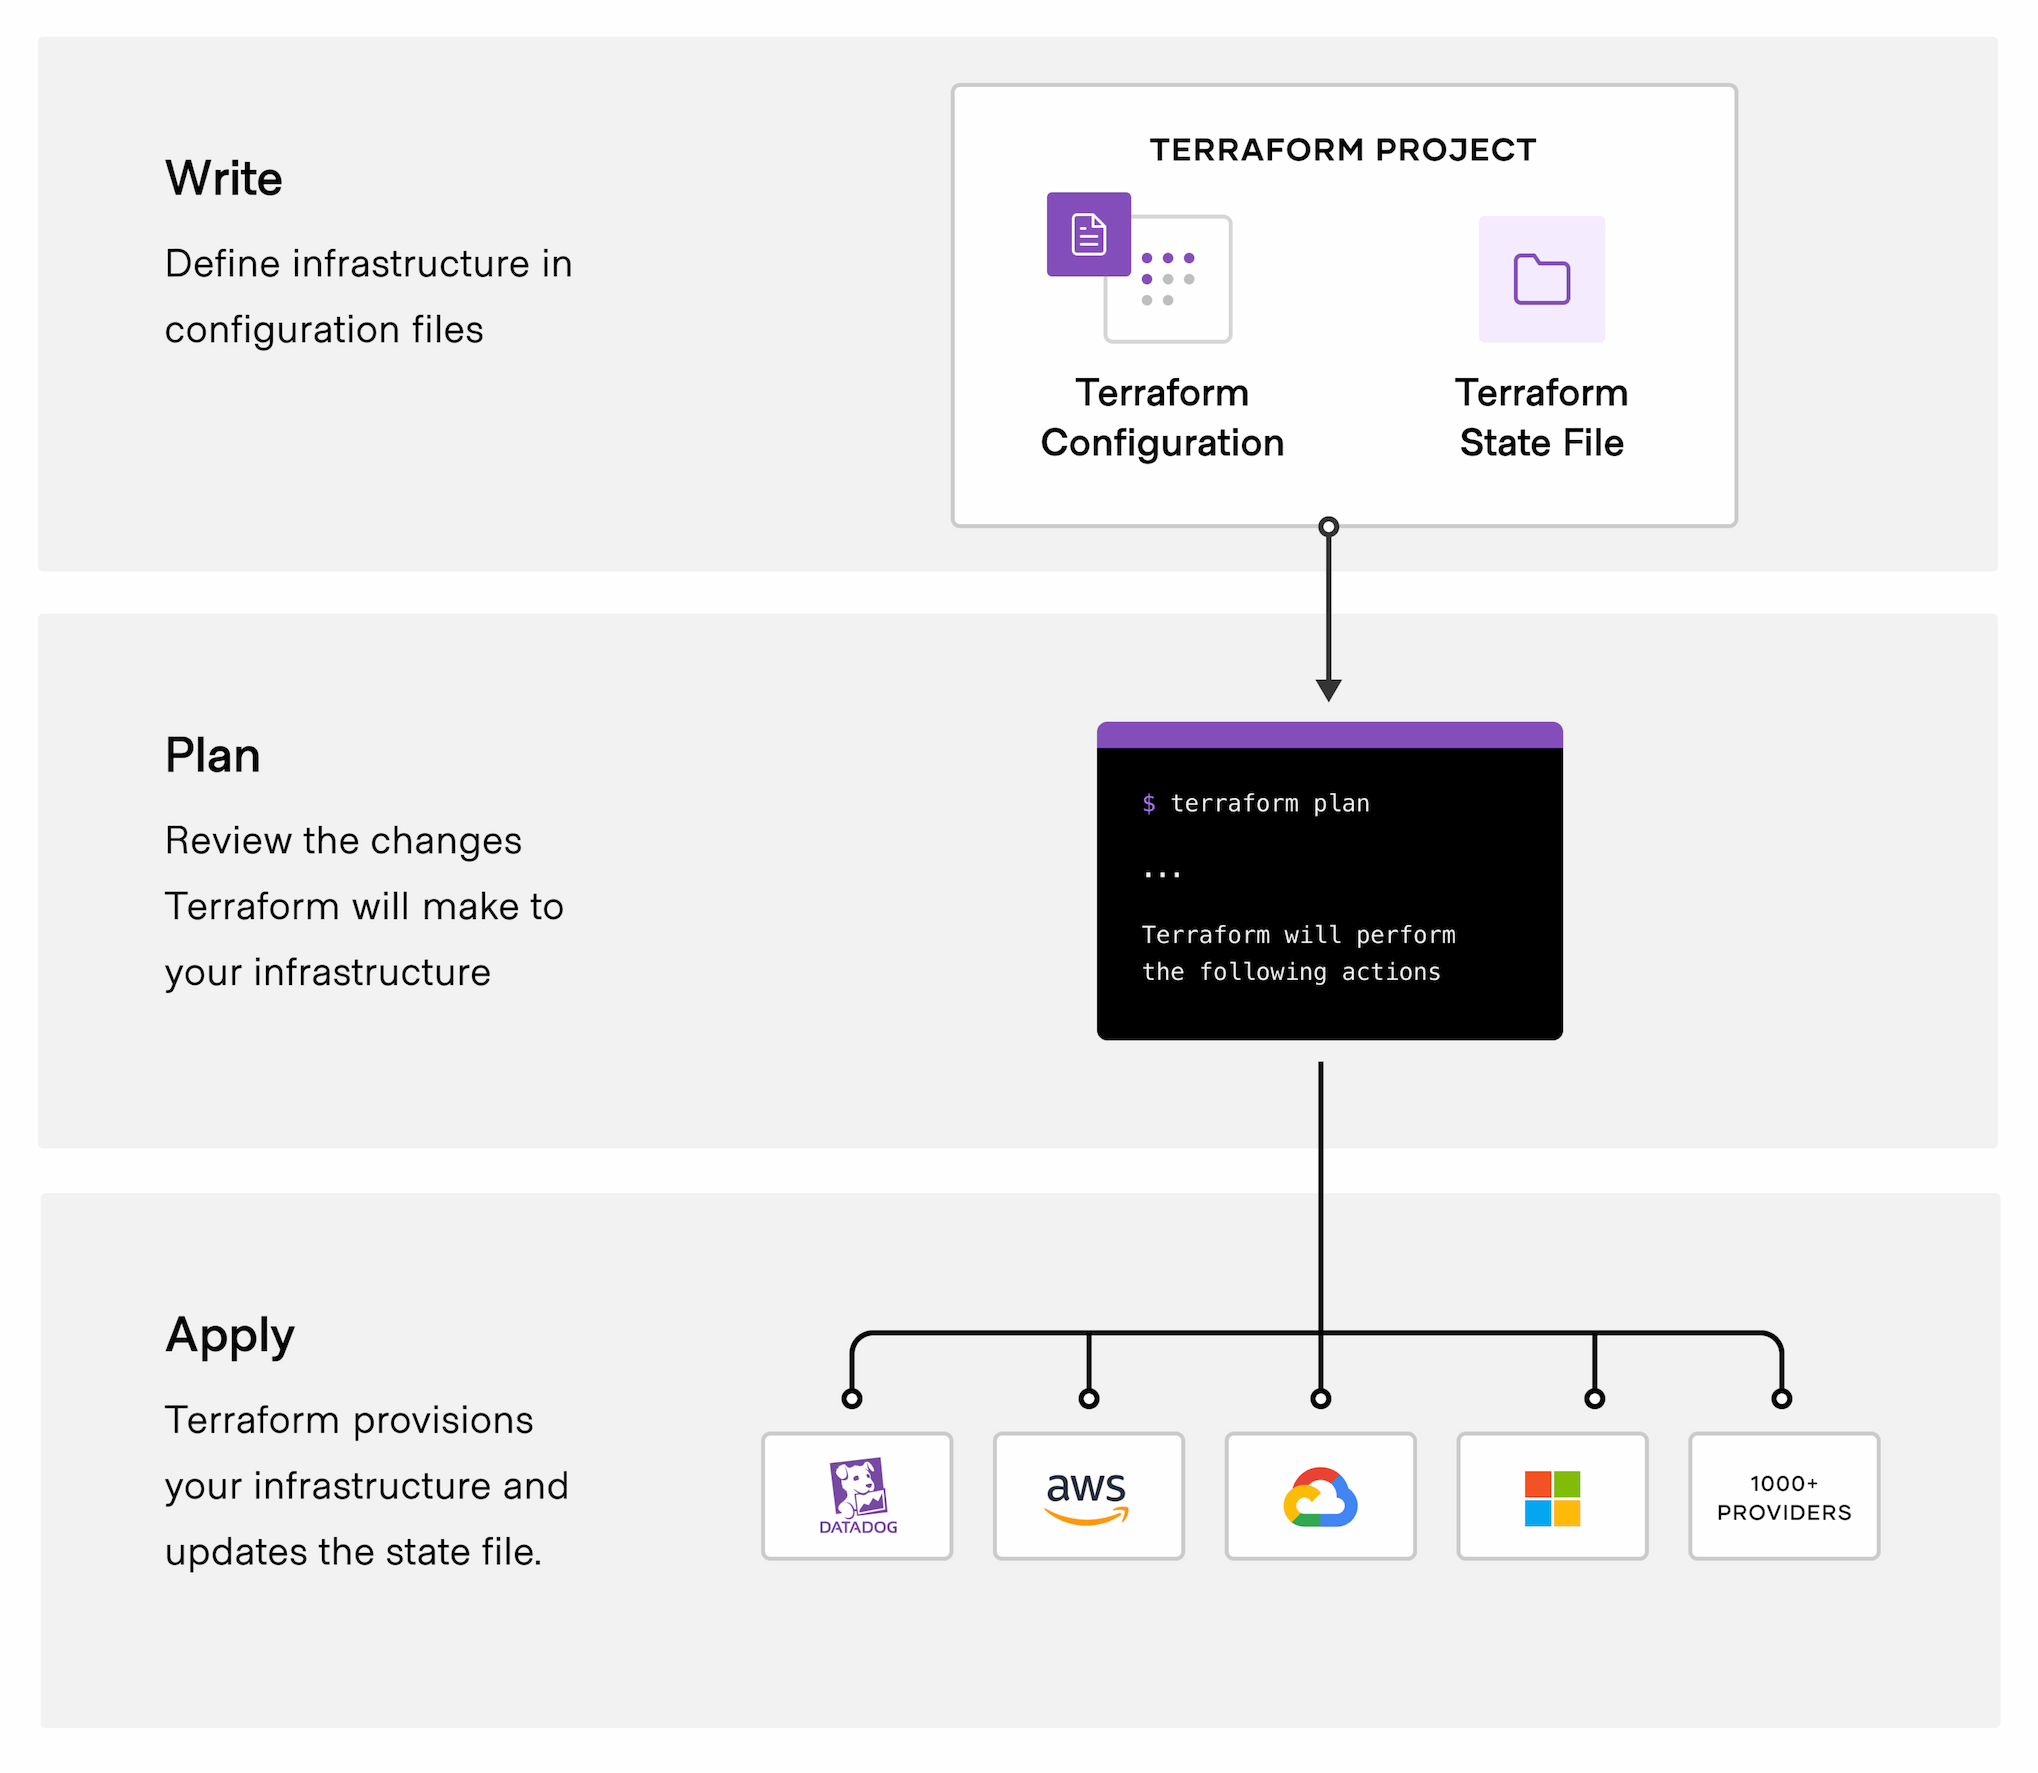
\includegraphics[width=0.6\textwidth]{figures/images/literature/terraformstages.png}}
                    \caption[Terraform Lépések]{Terraform Lépések~\footnotemark}
                    \label{fig:terraformstages}
                \end{figure}
                \footnotetext{\textit{Terraform}: \url{https://developer.hashicorp.com/terraform/intro/}}


        \subsection{Google Cloud Projekt - GCP}
        A rendszer cloud-oldali erőforrásai egyetlen Google Cloud Projektbe szervezett infrastruktúrán futnak, amelynek egyedi azonosítója \texttt{printermonitor-488112}.
        Az összes felhőszolgáltatás, az Artifact Registry-től a Vertex AI végpontig, a Cloud Function-öktől a Firestore adatbázisig, ezen a projekten belül van definiálva és menedzselve.
        A Google Cloud Platform (GCP) választásának fő indoka az volt, hogy egységes ökoszisztémát biztosít a gépi tanulási pipeline-hoz: a Vertex AI natívan integrálódik a Pub/Sub üzenetsorral,
        a Cloud Functions-szel és az Artifact Registry-vel, minimalizálva az integrációs komplexitást\cite{gcp}.
        Az erőforrások számlázása és a költségvetési riasztások szintén ezen a projekten belül vannak konfigurálva, lehetővé téve a kiadások szoros nyomon követését.

        \subsection{Vertex AI végpont}
        A Vertex AI végpont a detekciós pipeline magja: egy egyedi \texttt{judge} Docker konténert futtat, amelyen belül a betanított YOLOv8\cite{yolov8} modell végzi
        a képkockák valós idejű elemzését. A konténer induláskor betölti a modellt a \texttt{MODEL\_PATH} által megjelölt \texttt{best.pt} fájlból,
        majd egy HTTP szerveren (\texttt{/predict} végpont) vár a bejövő kérésekre.

        A szerver kétféle üzenetformátumot kezel: a Vertex AI natív \texttt{\{"instances": [...]\}} formátumát,
        amelyet a Dispatcher Cloud Function küld, valamint a Pub/Sub push formátumát.
        Minden beérkező képkockát Base64-ból visszaalakít, OpenCV-vel dekódol, majd a YOLO modellel elvégzi az objektumdetekciót.
        Az eredmény tartalmazza az észlelt hibaosztályokat (\texttt{label}), azok konfidenciaértékeit, valamint a határoló téglalapok
        koordinátáit mind pixel-, mind normalizált formában.

        A pillanatnyi téves riasztások szűrésére a konténer kameránként és hibaosztályonként számon tartja, hány egymást követő képkockán
        jelent meg ugyanaz a hiba. Egy detekció csak akkor minősül megerősítettnek, ha legalább \texttt{STREAK\_REQUIRED}
        (alapértelmezetten három) egymást követő képkockán át látható; ez kiszűri az egyetlen képkockán felvillanó, zajból eredő észleléseket.
        Mivel ez a számláló a folyamat memóriájában él, a végpontnak egyetlen, állandó példányon (\texttt{min} = \texttt{max} = 1 replika) kell futnia.

        A feldolgozott képkockát a konténer feltölti a \texttt{FRAMES\_BUCKET} névvel megadott GCS tárolóba, és az így kapott nyilvános URL-t a
        \texttt{frame\_url} mezőben csatolja az eredményhez, lehetővé téve, hogy a dashboard utólag a pontosan feldolgozott képet jelenítse meg.
        A detekciós eredmény ezt követően minden képkockára publikálásra kerül a \texttt{detections-out} Pub/Sub csatornára, beleértve azokat is,
        amelyeken nem történt észlelés; erre az adatra a dashboard inferencia-naplója támaszkodik.

        A végpont csak aktív használat közben generál költséget: tétlen (kitelepített, de nem hívott) állapotban nem számlázódik,
        míg folyamatos terhelés esetén napi körülbelül 37\$-os költséggel kell számolni.

        \subsection{Service Accounts}
        A szervíz felhasználók, olyan egyedi emailcímmel rendelkező entitások, melyek segítségével, különböző applikációk, virtuális gépek, vagy egyéb megvalósítások
        kommunikálhatnak a Google API-jával, emberi felhasználók helyett, ezzel biztonságos összeköttetést biztosítva a különböző erőforrások között.

            \subsubsection{sa-frame-extractor}
            \begin{sloppypar}
            A Raspberry Pi-n futó \texttt{frame-extractor} szolgáltatás ezzel a szervízfelhasználóval hitelesíti magát a Google Cloud felé.
            Szerepe, hogy a kinyert képkockák publikálhatóak legyenek a Pub/Sub üzenetbuszra. Jogosultságai: \texttt{pubsub.publisher}
            a \texttt{frames-in} csatornán, valamint \texttt{aiplatform.user} a Vertex AI végpont eléréséhez.
            \end{sloppypar}

            \subsubsection{sa-dispatcher}
            \begin{sloppypar}
            A \texttt{dispatcher} Cloud Function ezzel a szervízfelhasználóval fut. Feladata, hogy a beérkező képkockákat továbbítsa
            a Vertex AI végpontnak, és szükség esetén aktiválja az Alert-Managert. Jogosultságai: \texttt{aiplatform.user} a végpont
            meghívásához, \texttt{pubsub.subscriber} a \texttt{detections-out} csatornán, valamint \texttt{run.invoker} az Alert-Manager
            függvény meghívásához.
            \end{sloppypar}

            \subsubsection{sa-alert-manager}
            \begin{sloppypar}
            A figyelmeztetés kezelésért felelő, egyaránt az anomáliák észlelésekor, és a költségvetés meghaladásakor. Jogosultságai: \texttt{datastore.user},
            \texttt{eventarc.eventReceiver}, \texttt{pubsub.subscriber}, \texttt{run.invoker}.
            \end{sloppypar}

            \subsubsection{sa-cicd}
            \begin{sloppypar}
            A Terraform-infrastruktúra kézi szerkesztése nem ajánlott gyakorlat, ezért ezt egy automatizált GitHub Actions workflow végzi,
            amely ezzel a szervízfelhasználóval hitelesíti magát. Feladata az infrastruktúra kitelepítése és a \texttt{judge} konténer image
            feltöltése. Jogosultságai: \texttt{artifactregistry.writer}, \texttt{pubsub.admin}, \texttt{editor} és \texttt{iam.serviceAccountUser}.
            \end{sloppypar}
            \subsubsection{Vertex AI agent}
            \begin{sloppypar}
            A Vertex AI endpoint a \texttt{judge} (bíró) Docker konténer futtatásáért felelős. Jogosultságai:
            \texttt{pubsub.publisher} a \texttt{detections-out} csatornán.
            \end{sloppypar}

            \subsubsection{Pub/Sub agent}
            \begin{sloppypar}
            A Pub/Sub csatornák menedzselésére szolgál. Jogosultságai: \texttt{iam.serviceAccountTokenCreator}.
            \end{sloppypar}

        \subsection{Pub/Sub Topics}
        A Google Cloud Pub/Sub egy aszinkron üzenetközvetítő szolgáltatás, amely lehetővé teszi az alkalmazáskomponensek közötti laza csatolású kommunikációt\cite{pubsub}.
        A rendszer három darab Pub/Sub csatornát használ, melyek a következők: \texttt{frames-in}, mely a még nyers képkockákat továbbítja a Pi-től a Vertex AI végpont felé.
        A \texttt{detections-out}, mely a Vertex AI végpont által észlelt anomáliák eredményét továbbítja a dashboard felé, és a \texttt{budget-notifications}, mely figyelmeztet minket
        amennyiben átléptük a kiszabott költségvetést.
            
                

        \subsection{Google Cloud Függvények}
        A rendszer három Cloud Function (Gen2) példányt alkalmaz, amelyek Pub/Sub eseményekre triggerelődnek és kiszolgáltatás nélkül,
        skálázhatóan futnak. Mindhárom függvény az \texttt{sa-alert-manager}, illetve \texttt{sa-dispatcher} szervízfelhasználó jogosultságaival rendelkezik.

            \subsubsection{Dispatcher}
            A Dispatcher hidat képez az edge eszköz és a Vertex AI végpont között. A \texttt{frames-in} Pub/Sub csatornáról kap üzenetet,
            amelynek tartalma egy Base64-kódolt JPEG képkocka, a kamera azonosítója, egy szekvenciaszám és egy UTC időbélyeg.
            A függvény ezt az adatot a Vertex AI REST API-jára továbbítja (\texttt{/predict} végpont), OAuth2 Bearer tokennel hitelesítve.
            Ha a Vertex AI kérés hálózati hiba miatt meghiúsul, a függvény újra dobja a kivételt, így a Pub/Sub automatikusan újrapróbálkozik.
            A három Cloud Függvény közül ez a leginkább memóriaigényes, mivel képkockák bináris adatát szállítja HTTP-n keresztül.

            \subsubsection{Alert-Manager}
            A detekciós pipeline záró állomása. A \texttt{detections-out} csatornáról érkező minden üzenetet, a hiba nélkülieket is,
            naplóz a Firestore \texttt{inferences} kollekciójába, amely a dashboard inferencia-naplójának forrása. Ezt követően kiszűri azokat
            a detektált hibákat, amelyek konfidenciaértéke eléri a beállított küszöböt (alapértelmezetten 35\%). Az átmenő detektálásokat a Firestore
            \texttt{alerts} kollekcióba írja, rögzítve a kamera azonosítóját, az észlelt hibákat, az időbélyeget és a szekvenciaszámot.

            E-mail értesítést kizárólag magas súlyosságú hibaosztályok esetén küld: \texttt{spagetti}, \texttt{not\_sticking},
            \texttt{layer\_shift} és \texttt{warping}. Az ismétlődő riasztások elkerülése érdekében egyetlen, az egész rendszerre közös,
            300 másodperces visszatartási időt (\textit{cooldown}) alkalmaz, amelyet a Firestore \texttt{alert\_cooldowns} kollekciójában,
            a \texttt{global\_email} kulcs alatt tárol. A visszatartás csak akkor indul el, ha az e-mail ténylegesen kiment, így egy átmeneti
            SMTP-hiba nem nyomja el a következő riasztást. Az e-mail HTML formátumú, tartalmazza az észlelt hibák táblázatát és egy közvetlen linket a dashboardra.

            \subsubsection{Budget Notifier}
            E függvény célja, hogy megakadályozza a felhőköltségek elszabadulását. A \texttt{budget-notifications} Pub/Sub csatornán
            hallgatózik, amelyre a GCP saját költségvetési riasztó rendszere publikál, ha az előre beállított kiadási küszöb teljesül.
            A függvény az Alert-Managerrel közös kódbázisban van megvalósítva, és szintén cooldown mechanizmust alkalmaz.
            Az eseményt a Firestore \texttt{budget\_alerts} kollekcióba is naplózza, majd HTML e-mailben értesíti a felhasználót
            a felhasznált összegről és a küszöbértékről.

            
        \subsection{Firestore Collections}
        Az adatbáziskezelő rendszereknek két nagy fajtáját különböztetünk meg, a relációs adatbázisokat, és a nem relációs avagy NoSQL (Not only SQL) adatbázisokat.
        A fő különbség, hogy a relációs adatbázisokban az adatok táblákba rendezettek, és köztük jól meghatározott kapcsolatok vannak. Viszont a NoSQL adatbázisokban az
        adatok úgynevezett dokumentumokban vannak eltárolva, melyek szerkezete sokkal rugalmasabb és nem igényel előre meghatározott sémát. Mivel a projekt főként JSON formátumú
        adatokkal dolgozik, így a NoSQL adatbázisok sokkal jobban megfelelnek a céljainknak, és a Firestore egy igen népszerű és megbízható választás ezen a téren\cite{firestore}.

        A rendszer az alábbi Firestore kollekciókat és állapotdokumentumokat használja:

        \begin{itemize}
            \item Az \texttt{inferences} kollekció minden egyes feldolgozott képkocka inferencia-eredményét tárolja, a hiba nélkülieket is.
            Ez a kollekció szolgál a dashboard inferencia-naplójának adatforrásául, és a hozzá tartozó \texttt{frame\_url} mezőn keresztül
            a pontosan feldolgozott képkocka is visszanézhető.

            \item Az \texttt{alerts} kollekció tárolja a detektált anomáliák bejegyzéseit. Mezői: \texttt{camera\_id} (melyik kamera észlelte),
            \texttt{detections[]} (a hibák tömbje: név + konfidencia + bounding box), \texttt{timestamp} (mikor történt a detekció),
            \texttt{seq} (a képkocka szekvenciaszáma, amelyet a \texttt{frame-extractor} biztosít) és \texttt{created\_at} (mikor került be a bejegyzés).
            A dashboardon való hatékony keresést egy kompozit index segíti: \texttt{camera\_id ASC} + \texttt{timestamp DESC},
            azaz kamera szerint növekvő, időbélyeg szerint csökkenő sorrendben.

            \item Az \texttt{alert\_cooldowns} kollekció az e-mail értesítések visszatartási idejét kezeli. Egyetlen, az egész rendszerre közös
            \texttt{global\_email} kulcs alatt tárolja a legutóbbi sikeres küldés időpontját, megakadályozva a riasztás-özönt rövid időn belül ismétlődő anomáliák esetén.

            \item A \texttt{budget\_alerts} kollekció a GCP költségvetési riasztásokat naplózza, beleértve a felhasznált összeget,
            a beállított küszöböt és az esemény időbélyegét.

            \item A \texttt{system\_state/extraction} dokumentum tárolja a képkocka-rögzítés be- vagy kikapcsolt állapotát (\texttt{enabled} mező).
            A dashboardról az operátor állítja, a Raspberry Pi-n futó \texttt{frame-extractor} pedig ezt olvassa, így a rögzítés távolról szüneteltethető.
        \end{itemize}


        \subsection{Konténer képek}
        A Vertex AI végponton futó detekciós logika egy egyedi Docker konténer képbe (image) van csomagolva, melynek neve \texttt{judge}.
        Ez az image egy Python scriptet tartalmaz, amely induláskor betölti a betanított YOLOv8 modellt, majd várakozik a bejövő Pub/Sub üzenetekre.
        Egy üzenet érkezésekor kicsomagolja a base64-kódolt JPEG képkockát, elvégzi rajta az objektumdetekciót, majd az eredményt, a detektált hibaosztályokat és azok konfidenciaértékeit,
        visszapublikálja a \texttt{detections-out} Pub/Sub csatornára\cite{vertexai_custom_container}.
        Az image tárolása a Google Artifact Registry-ben történik, verziózva a commit SHA alapján.
        Minden módosítás esetén a \texttt{docker-judge.yml} GitHub Action automatikusan újrabuildi és feltölti a friss image-t, ahonnan a Vertex AI végpont azt lehúzza és futtatja.
        A konténer teljes életciklusát, a build fázistól a futtatásig, a \ref{fig:judge}. ábra mutatja be.

        \begin{figure}[H]
            \centering
            {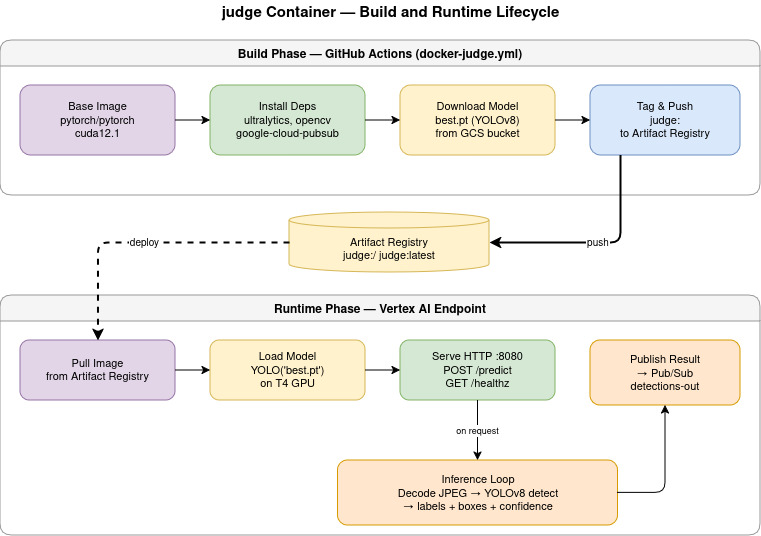
\includegraphics[width=\textwidth]{figures/images/literature/judge_cicd_pipeline.jpg}}
            \caption{A \texttt{judge} konténer image életciklusa}
            \label{fig:judge}
        \end{figure}

    \section{Dashboard}
    A rendszer felhasználói felülete egy webalkalmazás, melyet a Firebase Hosting platform szolgál ki,
    így külön szerver üzemeltetése nélkül érhető el a böngészőből\cite{firebase_hosting}. A felület két nézetből áll.

    Az első nézet (\textit{Live streams}) valós időben jeleníti meg a három kamera videofolyamát WebRTC technológia segítségével,
    a MediaMTX szerveren és a Cloudflare alagúton keresztül érkező RTSP streamekre támaszkodva. Erre a nézetre a Firebase Firestore
    adatbázishoz való közvetlen, valós idejű kapcsolaton keresztül (\texttt{onSnapshot} listener) kerülnek rá a nemrég megerősített
    detekciók jelölései; ezek néhány tíz másodperces késéssel követik az élő képet, mivel előbb végig kell haladniuk a teljes feldolgozási láncon.
    Ugyanitt található a rögzítés be- és kikapcsolására szolgáló vezérlő is, amelyet csak operátori Google-fiókkal bejelentkezve lehet
    használni; ez a \texttt{system\_state/extraction} dokumentumot írja, amelyet a Raspberry Pi olvas.

    A második nézet (\textit{Inference log}) az \texttt{inferences} kollekcióból építkezik: minden feldolgozott képkockához megjeleníti
    a hozzá tartozó képkocka-bélyeget és a detekciók táblázatát, a határoló téglalapokat pedig pontosan arra a képkockára rajzolja,
    amelyet a modell ténylegesen feldolgozott. Így ez a nézet képkocka-szinten hű képet ad a modell döntéseiről.

    A dashboard vizuálisan is visszajelzést ad a rendszer állapotáról: normál működés közben a felület semleges állapotot mutat
    (\ref{fig:dash_normal}. ábra), amennyiben pedig magas prioritású anomália érkezik, a felület piros kerettel jelenik meg
    (CSS \texttt{alerting} osztály aktiválásával), ahogy azt a \ref{fig:dash_high}. ábra szemlélteti.
    Hasonlóan, a költségvetési riasztás esetén sárga kerettel jelez (\texttt{budget-alert} osztály),
    így a felhasználó azonnal értesül a túllépésről anélkül, hogy az e-mailjét kellene ellenőriznie.

    \begin{figure}[H]
        \centering
        {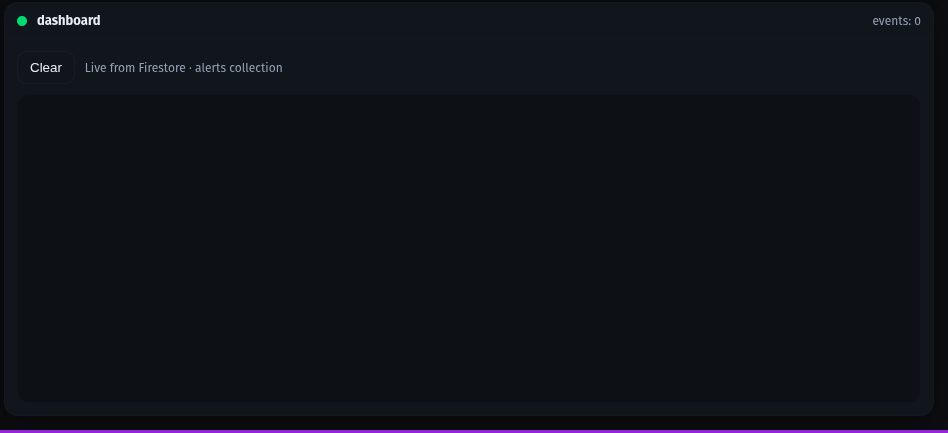
\includegraphics[width=\textwidth]{figures/images/literature/dash_normal.png}}
        \caption{A dashboard normál működési állapotban}
        \label{fig:dash_normal}
    \end{figure}

    \begin{figure}[H]
        \centering
        {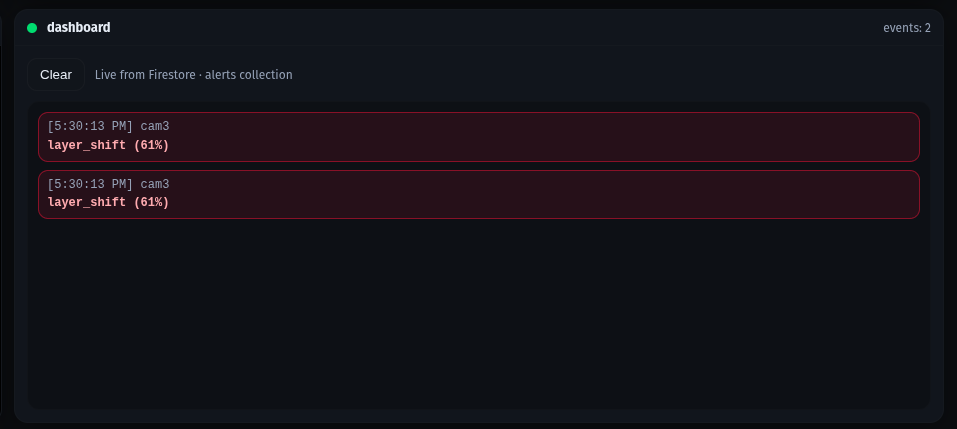
\includegraphics[width=\textwidth]{figures/images/literature/dash_high.png}}
        \caption{A dashboard anomália detektálás esetén}
        \label{fig:dash_high}
    \end{figure}

    \section{GitHub Action Workflows}
    A projekt folyamatos integrációját és automatizált kitelepítését (CI/CD) több GitHub Action workflow biztosítja,
    melyek a megfelelő kódváltozásra automatikusan lefutnak, csökkentve a manuális beavatkozás szükségességét és az emberi hibák esélyét\cite{github_actions}.
    Az infrastruktúra és a konténer kezelésén túl egy külön workflow (\texttt{python-tests.yml}) minden, a szolgáltatások kódját érintő változásnál
    lefuttatja a Python egységteszteket, és 90\%-os lefedettségi küszöböt vár el, egy további workflow (\texttt{compileLatex.yml}) pedig a dolgozat
    PDF-jét fordítja újra. Az alábbiakban a két fő, infrastruktúrát és konténert érintő workflow-t mutatjuk be részletesen.

        \subsection{Terraform lépések automatizálása}
        Ez a workflow a felhőinfrastruktúra változtatásait kezeli automatikusan.
        Pull request esetén csak ellenőrző lépések futnak le, hogy a változtatások biztonságosak és helyesek legyenek a merge előtt:
        a workflow lefuttatja a \texttt{terraform plan} parancsot, amelynek kimenetét egy emberi felülvizsgáló a pull request keretében
        ellenőrzi, mielőtt jóváhagyná az összevonást. Merge eseményre a \texttt{main} ágra a workflow elvégzi a tényleges infrastruktúra
        módosítást (\texttt{terraform apply}) a GCP-n.

        Megjegyzendő korlát, hogy a tervet (\texttt{plan}) és annak alkalmazását (\texttt{apply}) jelenleg a merge eseménye kapcsolja össze:
        a \texttt{main} ágra történő összevonás után az \texttt{apply} külön emberi megerősítés nélkül lefut. Robusztusabb megoldás lenne
        egy explicit, kézi jóváhagyási kapu (\textit{manual approval gate}) beiktatása közvetlenül az \texttt{apply} lépés elé, amely a
        ténylegesen alkalmazandó tervet még egyszer felülvizsgálatra bocsátja; ez a jövőbeli fejlesztések egyik iránya.

            \subsubsection{Konfigurációs ellenőrzés – Checkov}
            A Checkov egy nyílt forráskódú statikus elemző eszköz, amely Terraform konfigurációkat vizsgál ismert biztonsági problémák és rossz praktikák szempontjából\cite{checkov}.
            Futtatása pull request esetén kötelező lépés: amennyiben magas súlyosságú problémát talál, például nyilvánosan elérhető storage bucket vagy nem megfelelő IAM konfiguráció,
            a workflow megakadályozza a merge-t. Ez biztosítja, hogy a fejlesztés során se kerülhessen sérülékeny infrastruktúra a produkcióba.

            \subsubsection{Formázás és erőforráshasználat ellenőrzés-Lint}
            A linting lépés két dolgot ellenőriz. A \texttt{terraform fmt --check} parancs megvizsgálja, hogy a \texttt{.tf} fájlok formázása megfelel-e a Terraform hivatalos stílusirányelveknek.
            A \texttt{terraform validate} parancs pedig szintaktikailag és szemantikailag ellenőrzi a konfigurációt, kiszűrve a nem létező erőforrásokra való hivatkozásokat
            vagy érvénytelen argumentumokat. Ezzel a lépéssel a triviális hibák már a review fázisban kiszűrhetők.

        \subsection{Docker konténer felépítésének automatizálása}
        Ez a workflow a \texttt{judge} Docker image buildjeléért és az Artifact Registry-be való automatikus feltöltéséért felelős.
        Minden olyan push eseményre lefut, amely a \texttt{judge/} könyvtárat érinti, így csak releváns változtatás esetén indul el, nem feleslegesen.
        A workflow lépései sorban: hitelesítés az \texttt{sa-cicd} service account kulcsával, az image buildje, ellátása a commit SHA-val mint egyedi taggel,
        majd feltöltése a Google Artifact Registry-be. Ezt követően a Vertex AI végpont a következő aktiváláskor automatikusan az új image-t fogja használni.
        A két workflow együttes működését a \ref{fig:cicd}. ábra foglalja össze.

        \begin{figure}[H]
            \centering
            {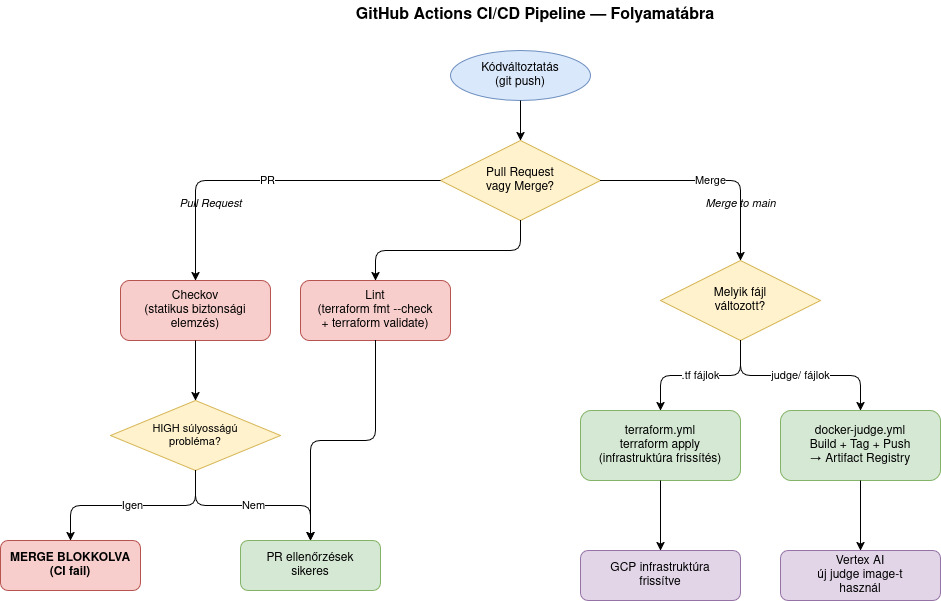
\includegraphics[width=\textwidth]{figures/images/literature/github_actions_cicd.jpg}}
            \caption{A CI/CD pipeline lépései}
            \label{fig:cicd}
        \end{figure}

    \section{Összefoglalás}
    A fejezet bemutatta a rendszer teljes hardver- és szoftverkörnyezetét.
    Az edge oldalon egy Raspberry Pi 4B gondoskodik a kameraképek rögzítéséről és valós idejű továbbításáról,
    a felhő oldalon pedig a Google Cloud Platform szolgáltatásai, Pub/Sub, Cloud Functions, Vertex AI, Firestore és Firebase Hosting,
    alkotják azt a pipeline-t, amely a nyers képkockáktól az anomáliadetekción át a felhasználói értesítésig minden lépést lefed.
    Az infrastruktúra Terraformmal van definiálva és verziókezelve, a CI/CD pipeline pedig biztosítja,
    hogy minden kódváltozás automatikusan, emberi beavatkozás nélkül jusson el az éles környezetbe.


\chapter{Adatgyűjtés és előfeldolgozás}
\section{Az adatgyűjtés folyamata}

A mélytanulási modellek betanításának alapfeltétele egy kellő méretű, változatos és reprezentatív
annotált képadathalmaz. Jelen projekt esetén ez különösen nehéz feladatnak bizonyult: az FDM
nyomtatási hibák vizuális megjelenése rendkívül változatos, függ a nyomtató típusától, a filament
anyagától és színétől, a megvilágítástól, a kamera szögétől és felbontásától, valamint a hiba
súlyosságától. Egy ilyen feltételek mellett általánosítható modell betanításához tehát nagy forrásvariabilitással rendelkező adathalmazra van szükség.

Az adatgyűjtés több párhuzamos forrásra támaszkodott: nyilvánosan elérhető adathalmazokra,
automatizált webes képletöltésre, valamint saját kezűleg rögzített felvételekre.

    \subsection{Nyilvánosan elérhető adathalmazok}

    Az adatgyűjtés első lépéseként három publikusan elérhető, 3D nyomtatási hibákat tartalmazó
    adathalmaz került felhasználásra.

    A Kaggle platformon Padraig Valenti által közzétett \textit{3D Printing Failure Detection}
    adathalmaz~\cite{kaggle_valenti} már YOLO-kompatibilis formátumban tartalmaz annotált képeket
    a legelterjedtebb FDM-hibatípusokra.

    A szintén Kaggle-ön elérhető, \textit{Mikulhe} felhasználó által megosztott \textit{3D Printing
    Errors}~\cite{kaggle_mikulhe} adathalmaz kiegészítő felvételeket biztosított, amelyek részben
    eltérő nyomtatókörnyezetből és megvilágítási feltételek mellől származnak, így növelve az
    adathalmaz vizuális diverzitását.

    A HuggingFace platformon a \textit{Javiai/failures-3D-print}~\cite{hf_javiai} adathalmaz
    további, különböző forrásból összegyűjtött hibás nyomtatásokat tartalmazó képeket nyújtott.

    \subsection{Webes képgyűjtés}

    A meglévő adathalmazok kiegészítéseképpen egyedi Python-szkript segítségével automatizált
    webes képletöltés is zajlott. A \texttt{imagescraper.py} szkript két üzemmódban képes működni:
    URL-listából történő közvetlen letöltés, illetve adott weboldal \texttt{<img>} tagjainak
    automatikus kinyerésével végzett oldalfeltérképezés (\textit{web crawling}).
    A letöltés aszinkron módon, az \texttt{aiohttp} könyvtár segítségével valósul meg, párhuzamos
    kapcsolatokkal, újrapróbálkozással és atomi fájlírással, megakadályozva a sérült vagy
    részleges letöltések bekerülését az adathalmazba. Az így összegyűjtött képek manuális
    szűrést követően kerültek az adathalmazba.

    \subsection{Saját felvételek}

    A külső forrásokból gyűjtött képanyagot 397 saját készítésű felvétellel egészítettük ki.
    Ezek valódi nyomtatási folyamatok közben, illetve szándékosan előidézett hibák dokumentálásával
    keletkeztek, a projekt által használt hardverkörnyezetben, azonos kameraelrendezéssel és
    megvilágítási feltételekkel. A saját képek bevonása azért bizonyult fontosnak, mert az
    adathalmaz így tartalmaz a rendszer tényleges működési körülményeihez közel álló felvételeket,
    amelyek segítenek csökkenteni a domain-eltolódás (\textit{domain shift}) hatását.

    Az összes forrásból összegyűjtött, manuálisan szűrt és előkészített adathalmaz az annotálás
    előtt összesen \textbf{2422 képből} állt.

% -------------------------------------------------------------------
\section{Annotálás}

    Az összegyűjtött képek annotálása a CVAT (\textit{Computer Vision Annotation Tool})~\cite{cvat}
    nyílt forráskódú platformon történt, kézi módszerrel. Minden képen az összes látható hibaterület
    körül határoló dobozt (\textit{bounding box}) rajzoltunk, amelyet a megfelelő osztálycímkével
    láttunk el.

    Az annotálás során alkalmazott kilenc osztály a következő:

    \begin{itemize}
        \item \textbf{stringing} - szálazás
        \item \textbf{warping} - vetemedés
        \item \textbf{layer\_shift} - réteg-eltolódás
        \item \textbf{under\_extrusion} - alul-extrúdálás
        \item \textbf{over\_extrusion} - felül-extrúdálás
        \item \textbf{nozzle\_clog} - fúvóka-dugulás
        \item \textbf{foreign\_object\_on\_print\_area} - idegen tárgy a tárgyasztalon
        \item \textbf{not\_sticking} - nem tapadó első réteg
        \item \textbf{spagetti} - spagetti-jelenség
    \end{itemize}

    A \ref{fig:training_grid}. ábra az egyes hibaosztályokhoz tartozó egy-egy reprezentatív tanítóképet mutat be.

    \begin{figure}[H]
    \centering
        \subfigure[szálazás]{
            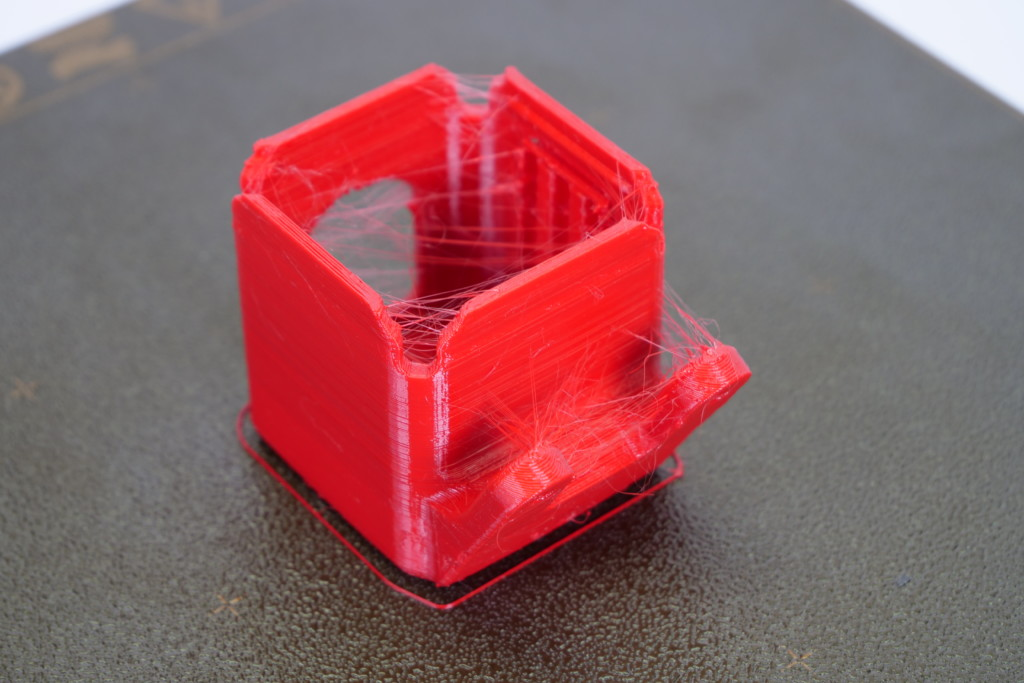
\includegraphics[width=0.3\textwidth]{figures/images/training_samples/stringing.jpg}
        }
        \subfigure[vetemedés]{
            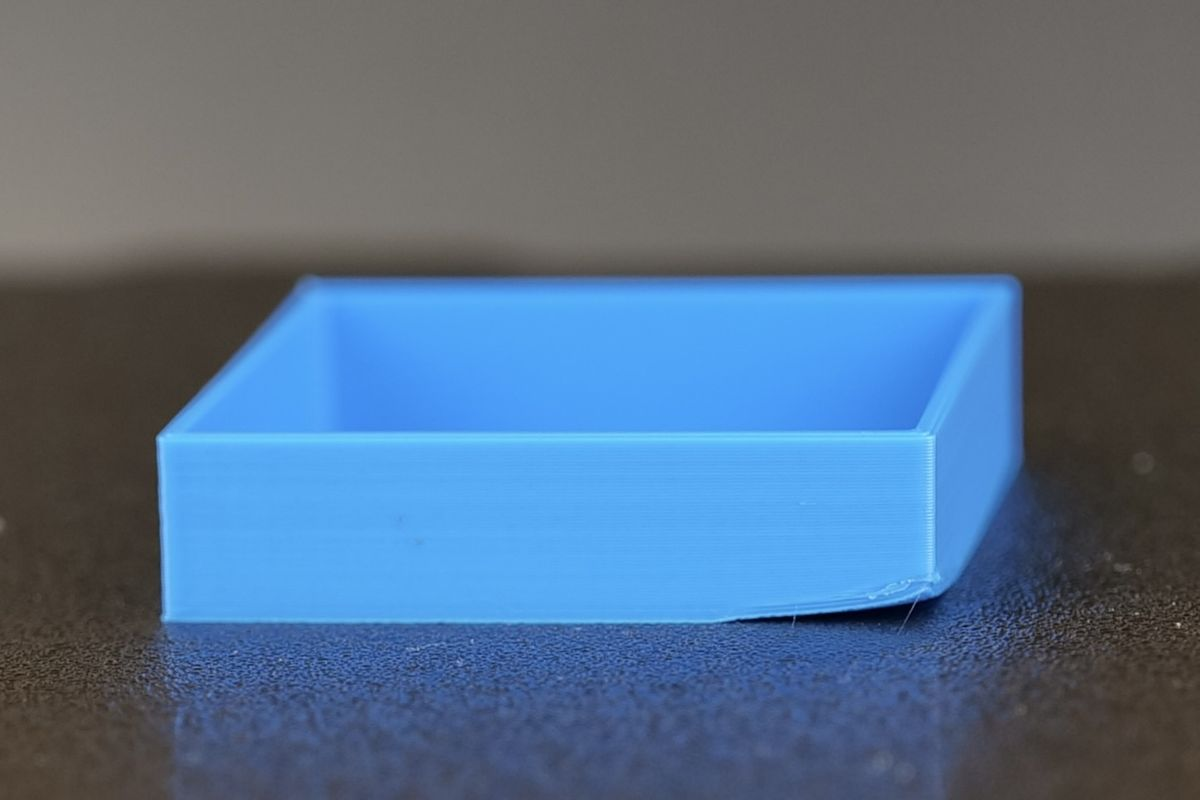
\includegraphics[width=0.3\textwidth]{figures/images/training_samples/warping.jpg}
        }
        \subfigure[réteg eltolódás]{
            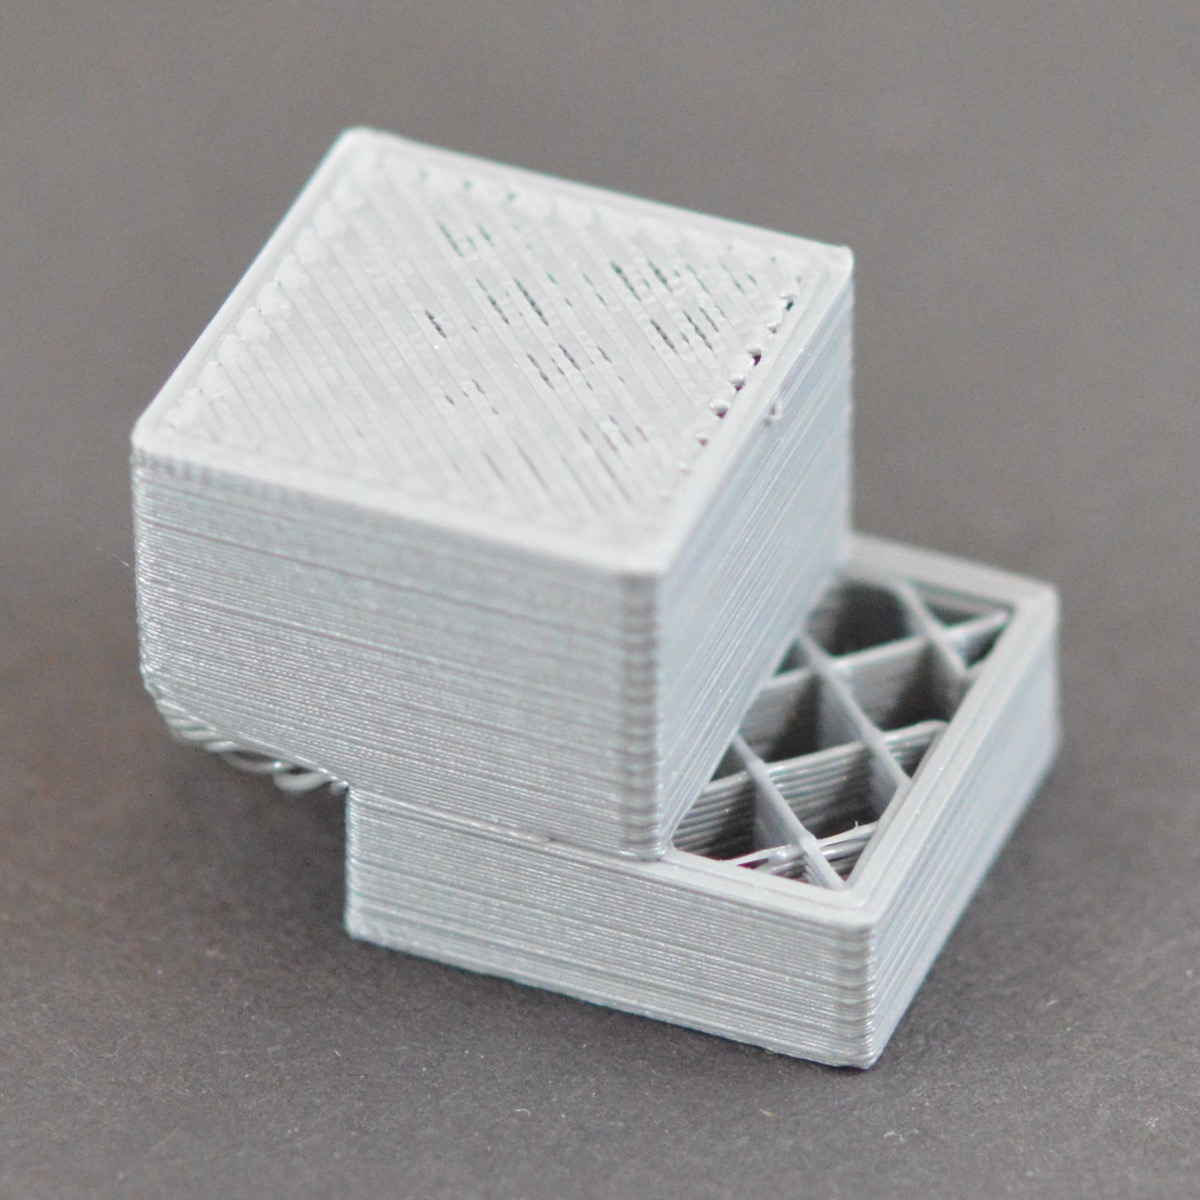
\includegraphics[width=0.3\textwidth]{figures/images/training_samples/layer_shift.jpg}
        }

        \subfigure[alul extrúdálás]{
            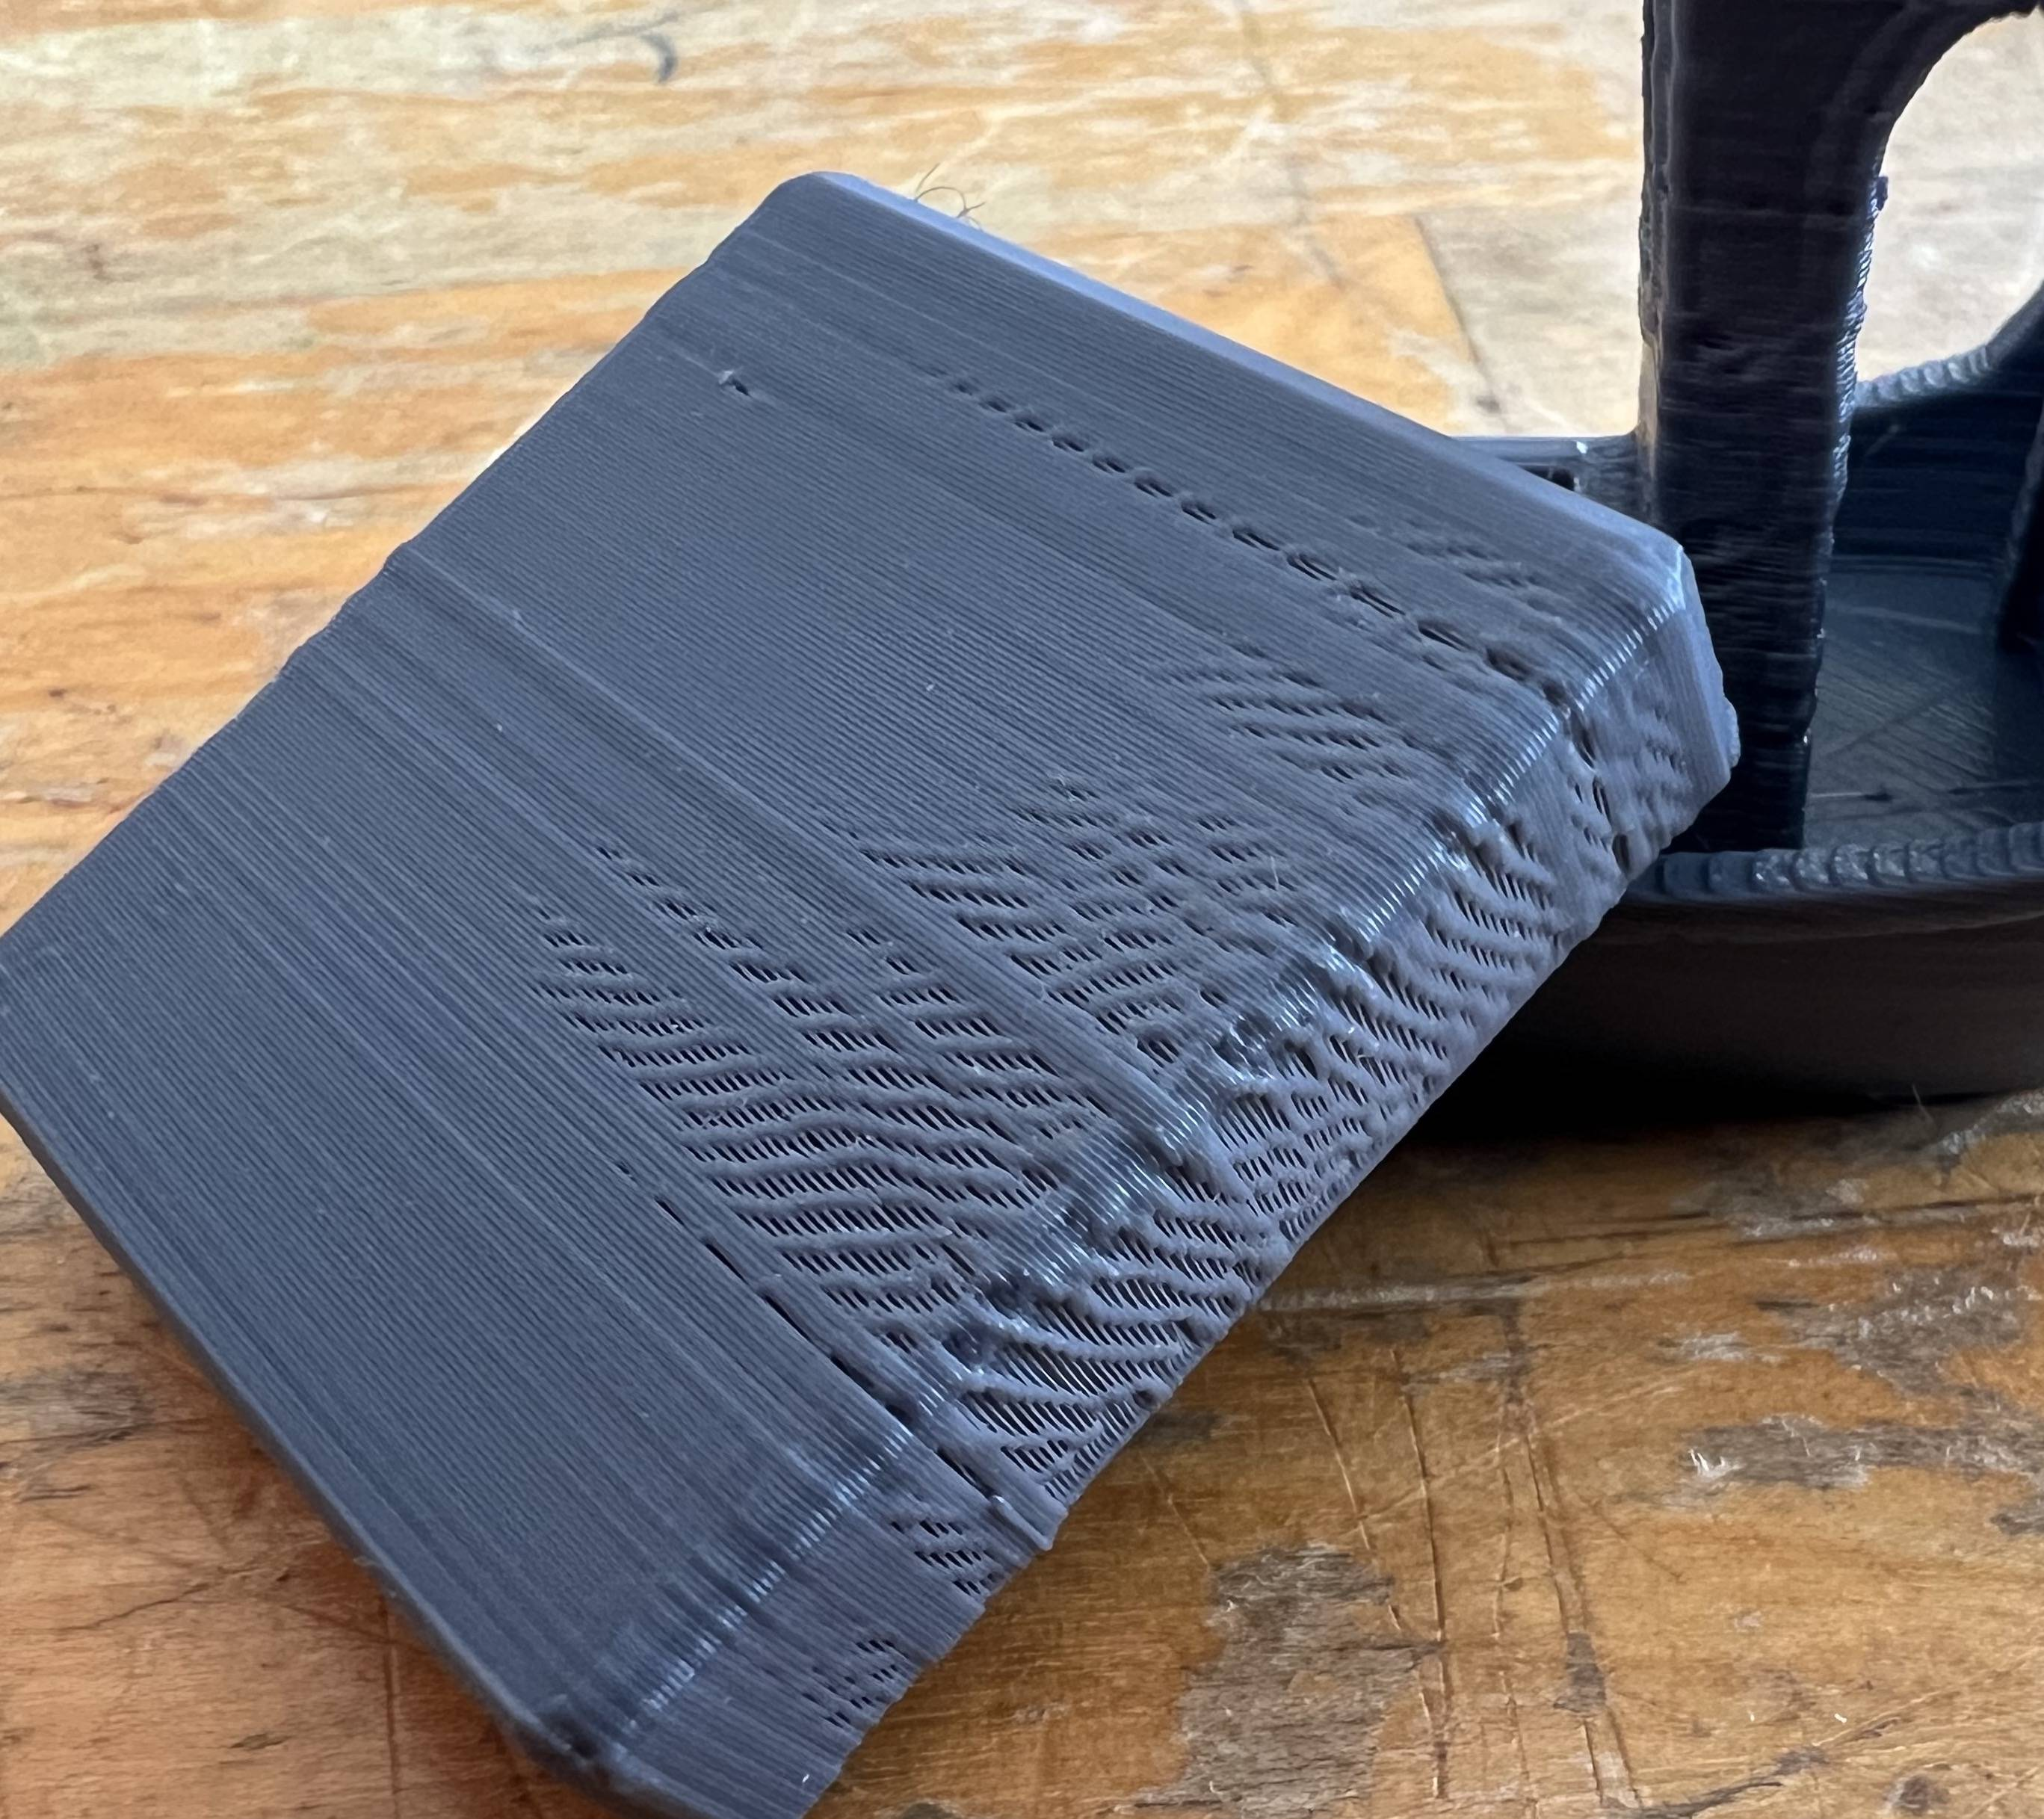
\includegraphics[width=0.3\textwidth]{figures/images/training_samples/under_extrusion.jpg}
        }
        \subfigure[felül extrudálás]{
            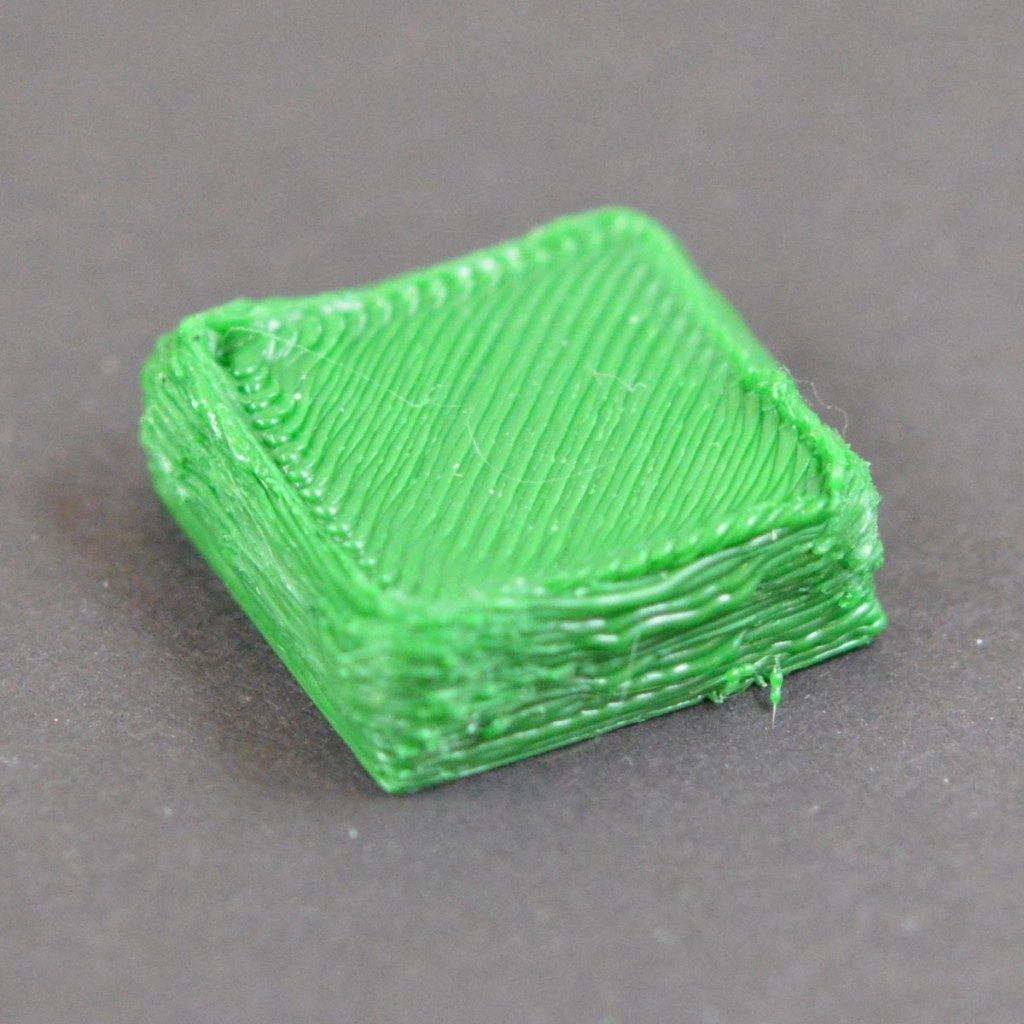
\includegraphics[width=0.3\textwidth]{figures/images/training_samples/over_extrusion.jpg}
        }
        \subfigure[fúvóka dugulás]{
            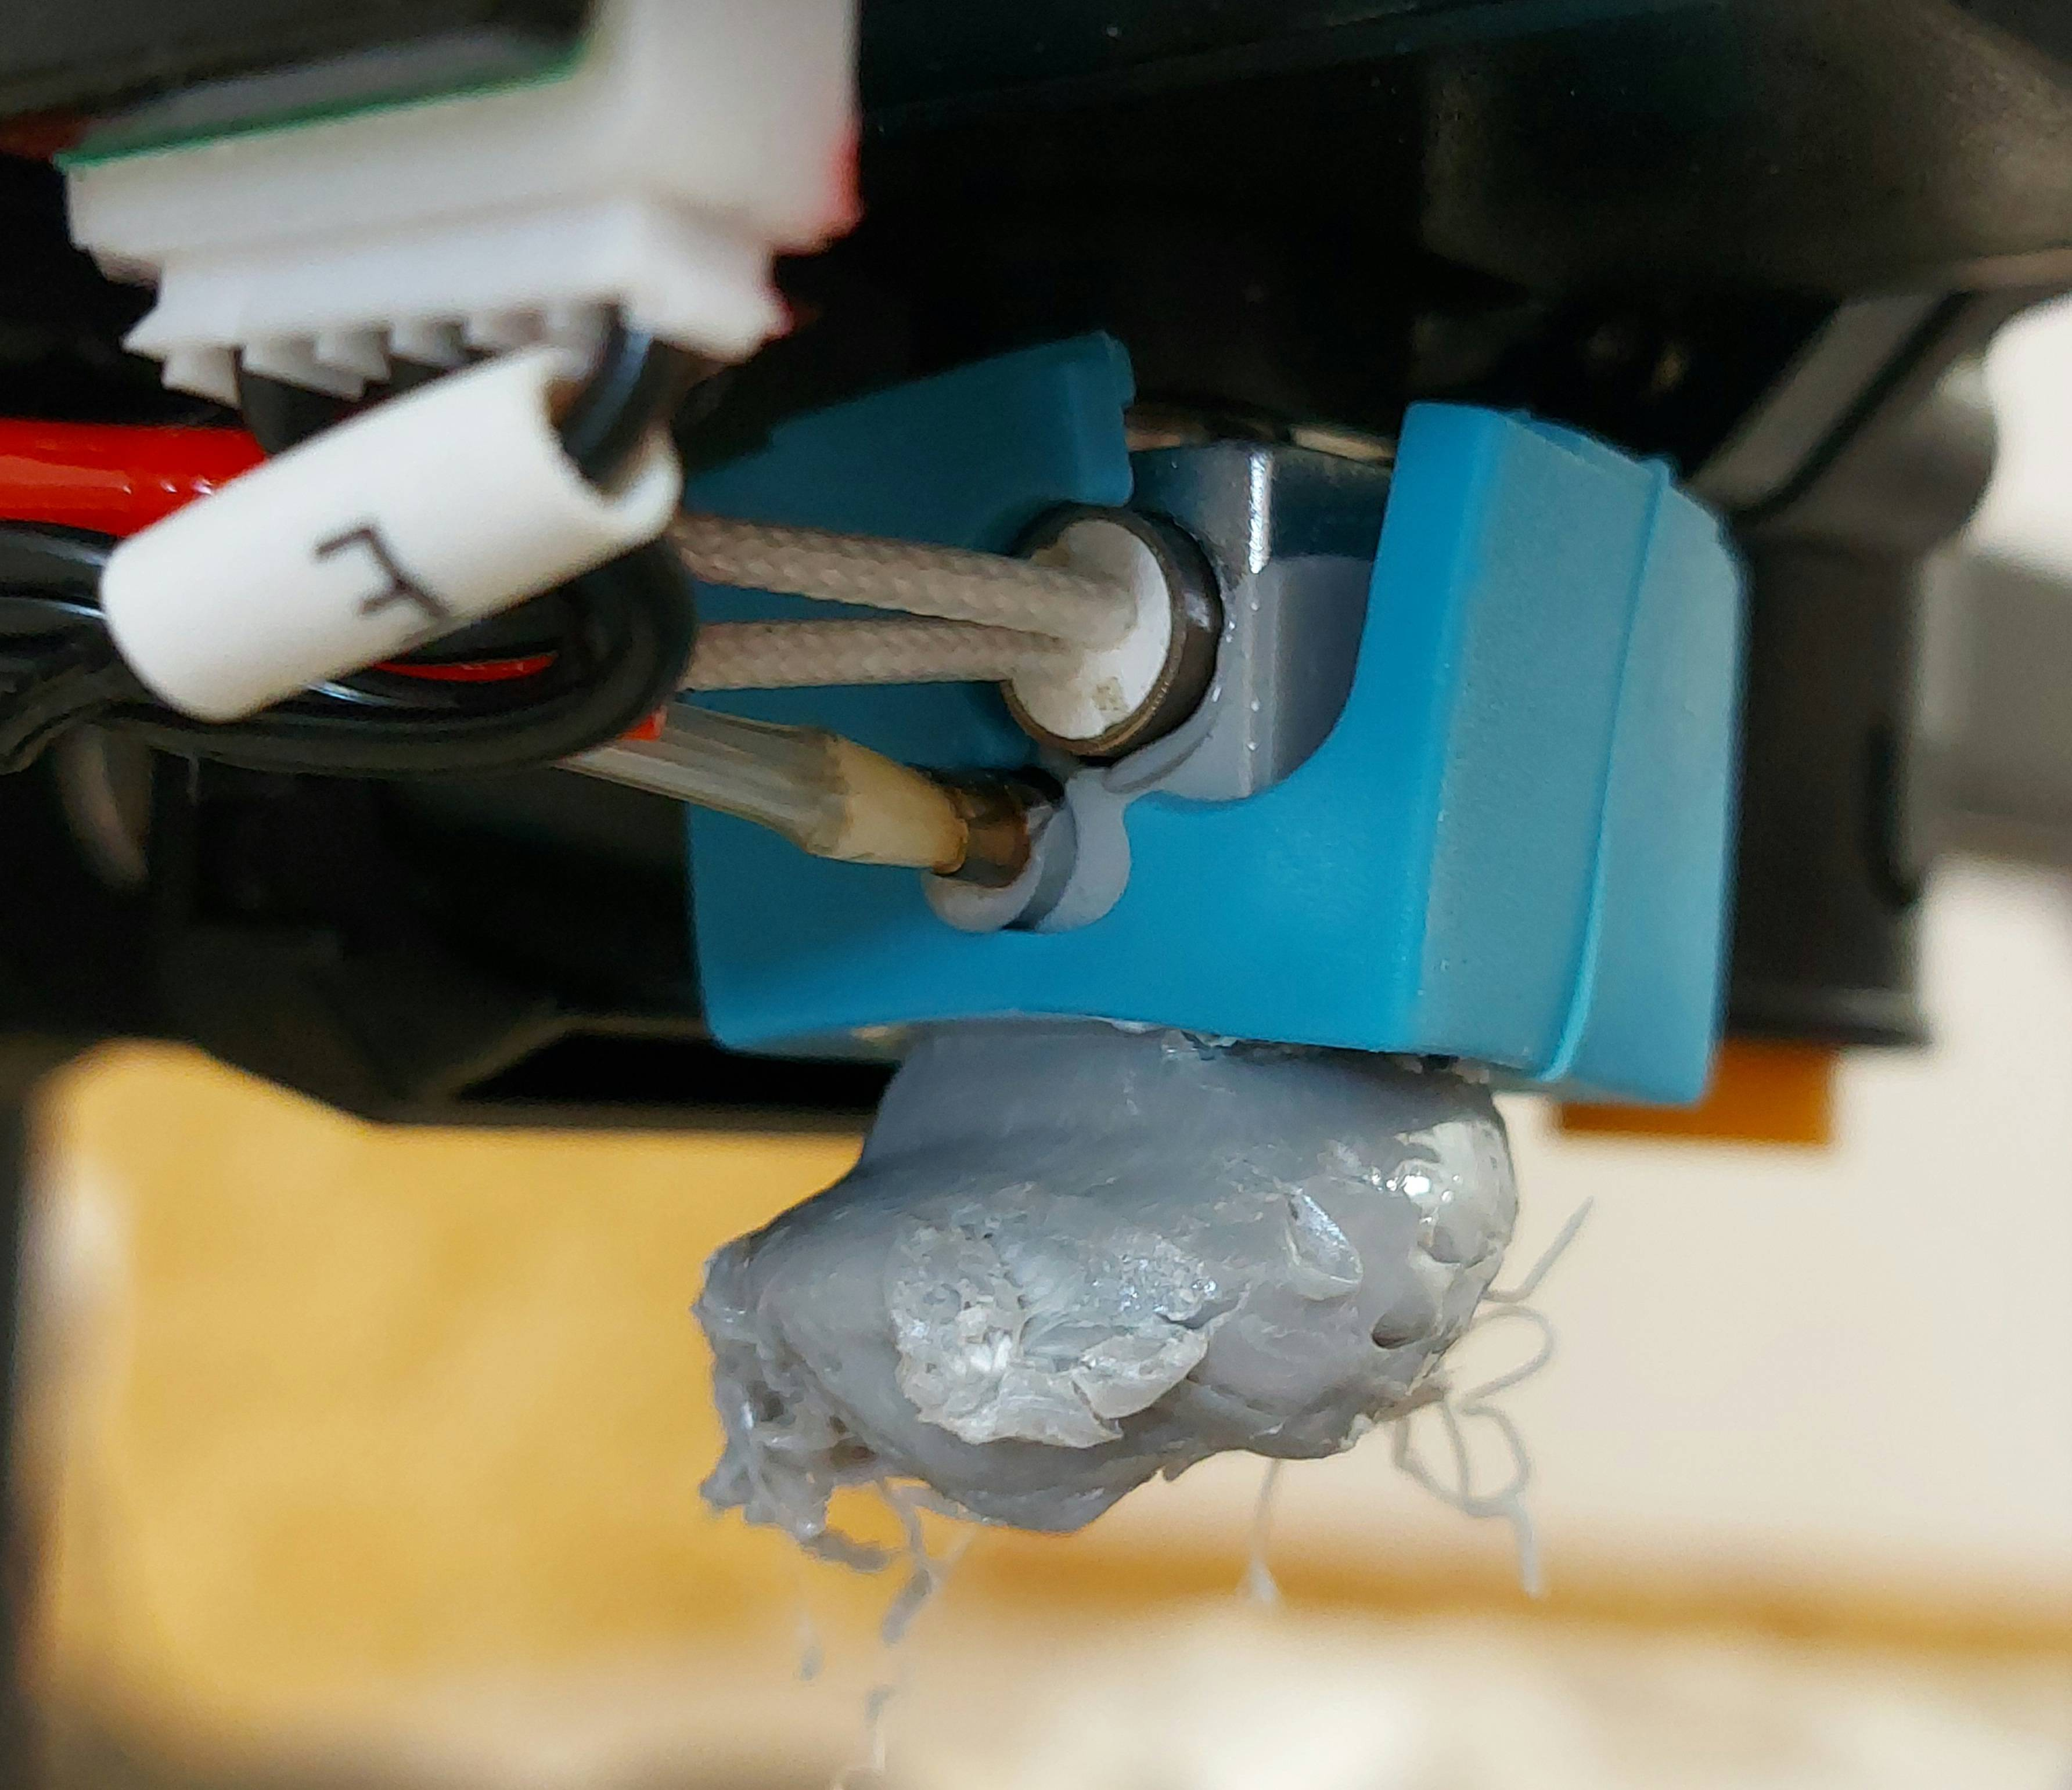
\includegraphics[width=0.3\textwidth]{figures/images/training_samples/nozzle_clog.jpg}
        }

        \subfigure[idegen tárgy]{
            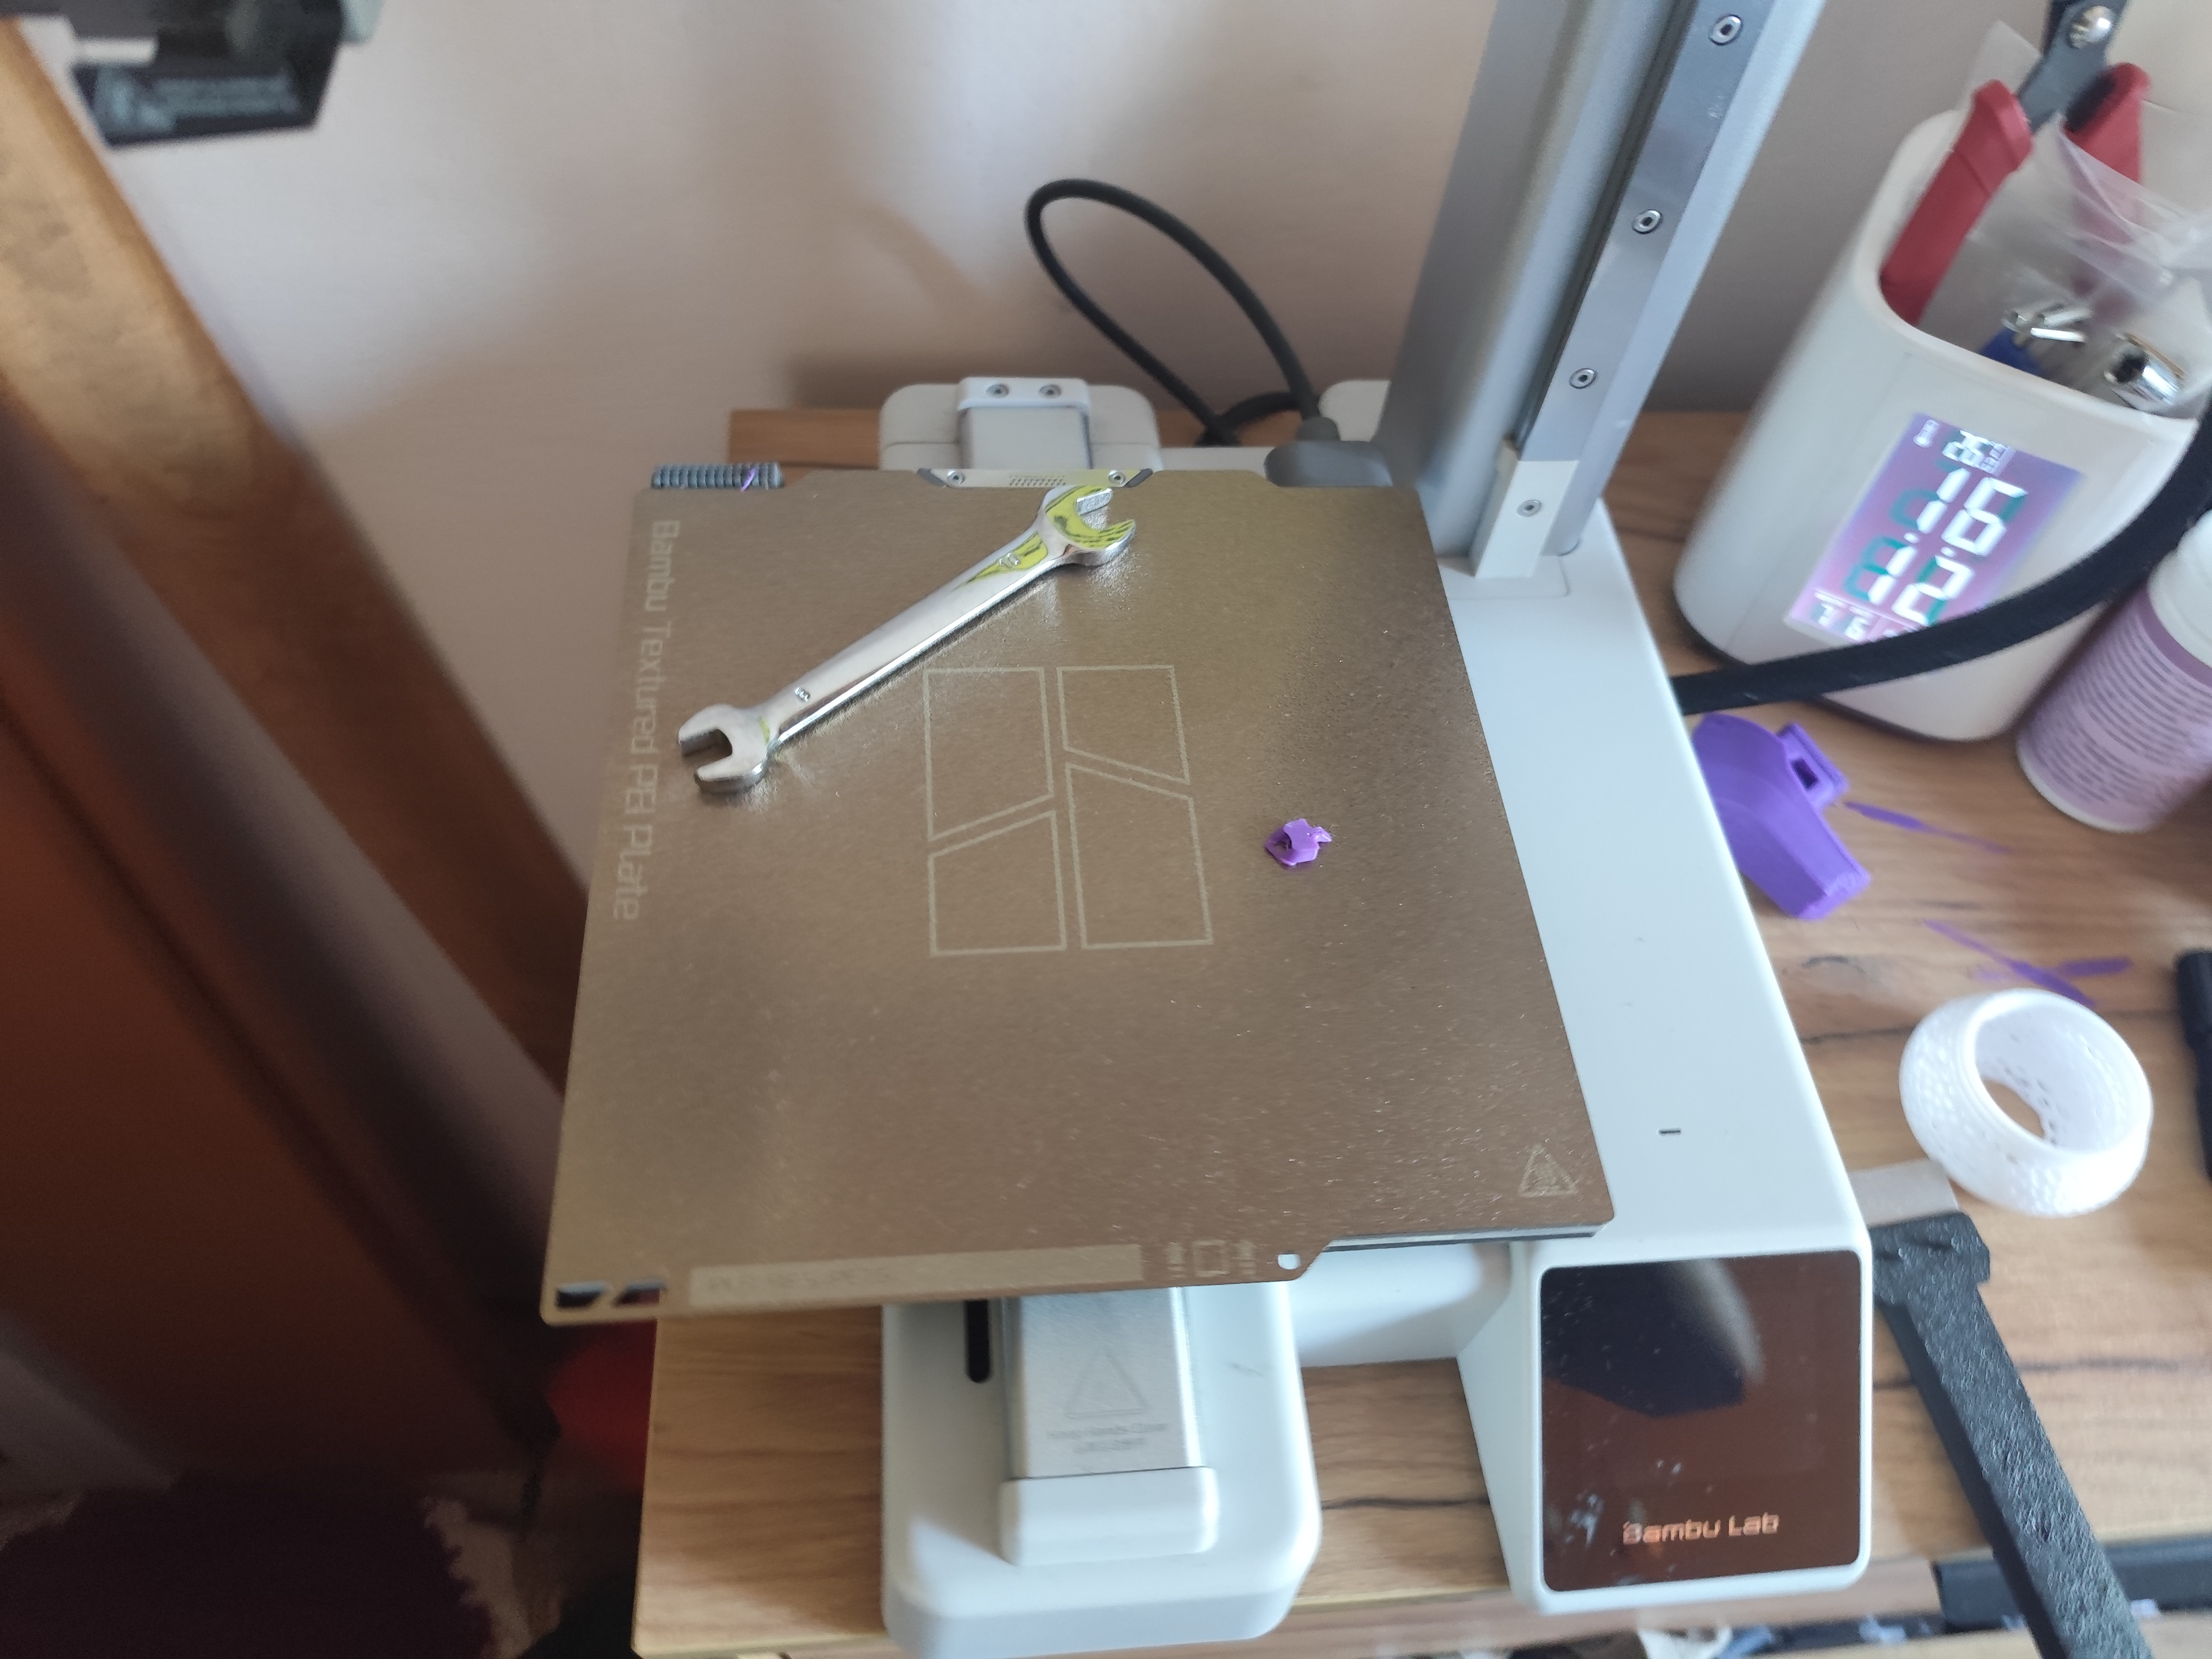
\includegraphics[width=0.3\textwidth]{figures/images/training_samples/foreign_object.jpg}
        }
        \subfigure[nem tapadó első réteg]{
            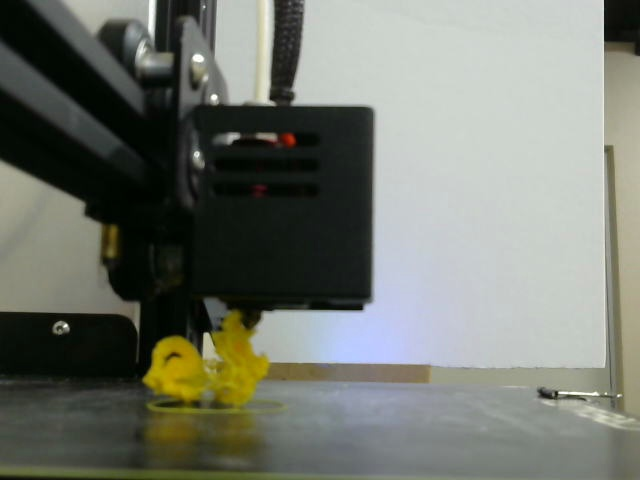
\includegraphics[width=0.3\textwidth]{figures/images/training_samples/not_sticking.jpg}
        }
        \subfigure[spagetti]{
            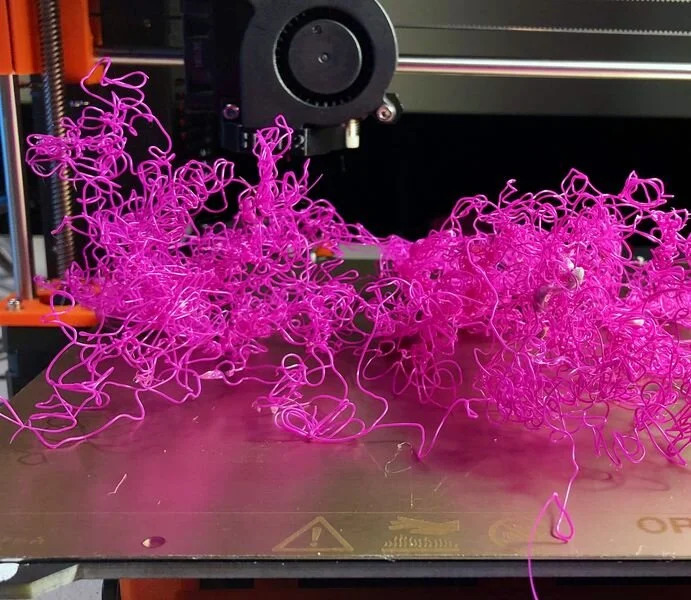
\includegraphics[width=0.3\textwidth]{figures/images/training_samples/spagetti.jpg}
        }
    \caption{Reprezentatív tanítóképek a kilenc hibaosztályból}
    \label{fig:training_grid}
    \end{figure}

    A CVAT az annotációkat YOLO-formátumban exportálta: minden képhez egy \texttt{.txt} fájl
    tartozik, amelynek minden sora egy detektált objektumot ír le az
    \texttt{<osztály> <x\_közép> <y\_közép> <szélesség> <magasság>} normalizált formátumban,
    ahol a koordináták a képmérethez viszonyítva 0 és 1 közé esnek.

    Az annotálás a projekt egyik legtöbb időt igénylő szakasza volt, mivel minden határolódobozt
    manuálisan kellett elhelyezni és az osztálycímkét hozzárendelni, különös figyelmet fordítva
    arra, hogy a több hibatípust egyidejűleg mutató képeken minden látható defektust helyesen
    azonosítsunk.

% -------------------------------------------------------------------
\section{Adathalmaz-előfeldolgozás}

    \subsection{Train/val felosztás}

    Az annotált adathalmazt a \texttt{splitter.py} szkript segítségével osztottuk szét tanító-
    és validációs részhalmazra, \textbf{80/20 arányban}. A felosztás reprodukálhatósága érdekében
    rögzített véletlenszám-magot (\texttt{seed = 42}) alkalmaztunk. Az eredményül kapott mappa-
    struktúra közvetlenül kompatibilis a YOLOv8 betanítási pipeline-jával:
    \texttt{images/train}, \texttt{images/val}, \texttt{labels/train}, \texttt{labels/val}.

    \subsection{Osztályegyensúly-korrekció - oversampling}

    Az adathalmazban a kilenc hibaosztály előfordulása nem egyenletes: egyes ritkábban előforduló
    vagy nehezebben dokumentálható hibatípusok, például a \textit{nozzle\_clog} vagy a
    \textit{foreign\_object\_on\_print\_area}, lényegesen kevesebb példánnyal szerepelnek,
    mint a gyakoribb kategóriák. Az osztályegyensúlyhiány közvetlen hatással van a modell
    tanulási dinamikájára: az alulreprezentált osztályok felismerési pontossága alacsonyabb lesz.

    Ennek korrekciójára az \texttt{oversample\_train.py} szkript osztályalapú oversamplinget
    hajt végre a tanítókészleten: minden olyan osztálynál, amelynek instanciaszáma egy meghatározott
    küszöbérték alatt marad, véletlenszerűen kiválasztott, adott osztályt tartalmazó képeket
    másol be új névvel a tanítókészletbe, legfeljebb tíz másolatot képenként, mindaddig,
    amíg a célszám el nem érhető. Ezzel az eljárással a modell az alulreprezentált hibatípusokon
    is elegendő tanulási példán tud végigmenni.

    \subsection{Adataugmentáció}

    Az adathalmaz méretének és vizuális variabilitásának növelésére automatizált augmentációs
    pipeline-t alkalmaztunk az \texttt{augment.py} szkript formájában. A szkript minden egyes
    tanítóképből alapértelmezés szerint \textbf{4 augmentált változatot} állít elő, háromféle
    augmentációs stratégia valamelyikét alkalmazva:

    \begin{itemize}
        \item \textbf{Alaptranszformációk} (~70\% valószínűséggel): Az Albumentations könyvtár
        segítségével véletlenszerű vízszintes és függőleges tükrözés, fényerő- és
        kontrasztváltoztatás, telítettség- és árnyalateltolás, Gauss-elmosás, léptékváltoztatás
        és forgatás kerül alkalmazásra, mindig a határoló dobozokat is megfelelően transzformálva.

        \item \textbf{Smart MixUp} (~20\% valószínűséggel): Két, egymással vizuálisan kompatibilis
        osztálypárt tartalmazó kép súlyozott lineáris keverékeként (\(\lambda \in [0{,}4;\,0{,}6]\))
        új szintetikus képet állít elő, amelyhez mindkét forráskép annotációi megmaradnak.
        Az összekeverhető osztálypárokat előre definiált kompatibilitási lista szabályozza,
        elkerülve a vizuálisan ellentmondásos kombinációkat.

        \item \textbf{Mozaik (\textit{Mosaic})} (~10\% valószínűséggel): Négy véletlenszerűen
        kiválasztott kép egy 640×640 pixeles vászonra kerül egymás mellé, negyed-negyed területre
        skálázva. Az így keletkező mozaikkép határoló dobozainak koordinátái átszámításra kerülnek
        az új pozícióra, megőrizve a teljes annotációt.
    \end{itemize}

    Minden augmentáció után az összes határoló doboz koordinátáit $[0, 1]$ közé visszavágjuk
    (\textit{clamping}), megelőzve az érvénytelen YOLO-annotációk keletkezését. A 4-szeres
    szorzóval végzett augmentáció eredményeként a tanítókészlet közel \textbf{négyszeresére}
    bővült, miközben a validációs halmazon augmentáció nem történt, annak érdekében, hogy
    a kiértékelés valódi, módosítatlan képeken menjen végbe.



\chapter{Modell betanítása és validálása}
\section{A kétfázisú tanítási stratégia}

A modell betanítása két egymást követő fázisban zajlott. Az első fázisban (\texttt{y8x\_phase1\_960}) a YOLOv8x alap előtanított
súlyokból kiindulva, 960 képpontos bemeneti felbontáson tanítottuk be a modellt az összegyűjtött adathalmazon. A második
fázisban (\texttt{y8x\_phase2\_12803}) az első fázis legjobb súlyait (\texttt{best.pt}) töltöttük be kiindulópontként, majd
finomhangolást végeztünk 1280 képpontos felbontáson, 100 epokon keresztül. Ez a megközelítés lehetővé tette, hogy a modell
először általánosabb jellemzőket tanuljon meg alacsonyabb felbontáson, majd a magasabb felbontású finomhangolás során
részletgazdagabb mintázatokat, például finom szálhúzásokat vagy rétegcsúszásokat, is megbízhatóan felismerjen.

\section{A második tanítási fázis konfigurációja}

A második fázis főbb hiperparamétereit az alábbi táblázat foglalja össze:

\begin{table}[H]
\centering
\caption{A \texttt{y8x\_phase2\_12803} tanítási konfiguráció főbb paraméterei}
\label{tab:phase2_config}
\renewcommand{\arraystretch}{1.4}
\begin{tabular}{|l|l|}
    \hline
    \textbf{Paraméter} & \textbf{Érték} \\
    \hline
    Kiindulómodell & \texttt{y8x\_phase1\_960/weights/best.pt} \\
    \hline
    Epokszám & 100 \\
    \hline
    Bemeneti felbontás & $1280 \times 1280$ px \\
    \hline
    Batch méret & 4 \\
    \hline
    Optimalizáló & AdamW \\
    \hline
    Kezdő tanulási ráta (\texttt{lr0}) & $2 \times 10^{-4}$ \\
    \hline
    Végső tanulási ráta (\texttt{lrf}) & $0{,}01$ \\
    \hline
    Tanulási ráta ütemező & Koszinuszos csökkentés (\texttt{cos\_lr}) \\
    \hline
    Dropout & $0{,}1$ \\
    \hline
    Korai leállítás türelme & 40 epok \\
    \hline
    Adataugmentáció & Mozaik, mixup, copy-paste, RandAugment, erasing \\
    \hline
\end{tabular}
\end{table}

A tanítás során a modell automatikus adataugmentációt alkalmazott, amely magában foglalta a mozaikszerű
képösszeállítást (\textit{mosaic}), a képkeverést (\textit{mixup}, arány: $0{,}1$), a másolás-beillesztés augmentációt
(\textit{copy-paste}, arány: $0{,}2$), a RandAugment eljárást, valamint véletlenszerű törlési területeket (\textit{erasing},
$0{,}3$). A geometriai transzformációk között szerepelt $\pm10^{\circ}$-os forgatás, $0{,}7$-es skálázás, $0{,}2$-es eltolás,
valamint vízszintes és függőleges tükrözés. A magas felbontás és az erőteljes augmentációs stratégia együttesen
csökkentette a túltanulás kockázatát.

\section{Tanítási eredmények és metrikák}

\subsection{Veszteség- és metrikagörbék}

\begin{figure}[H]
    \centering
    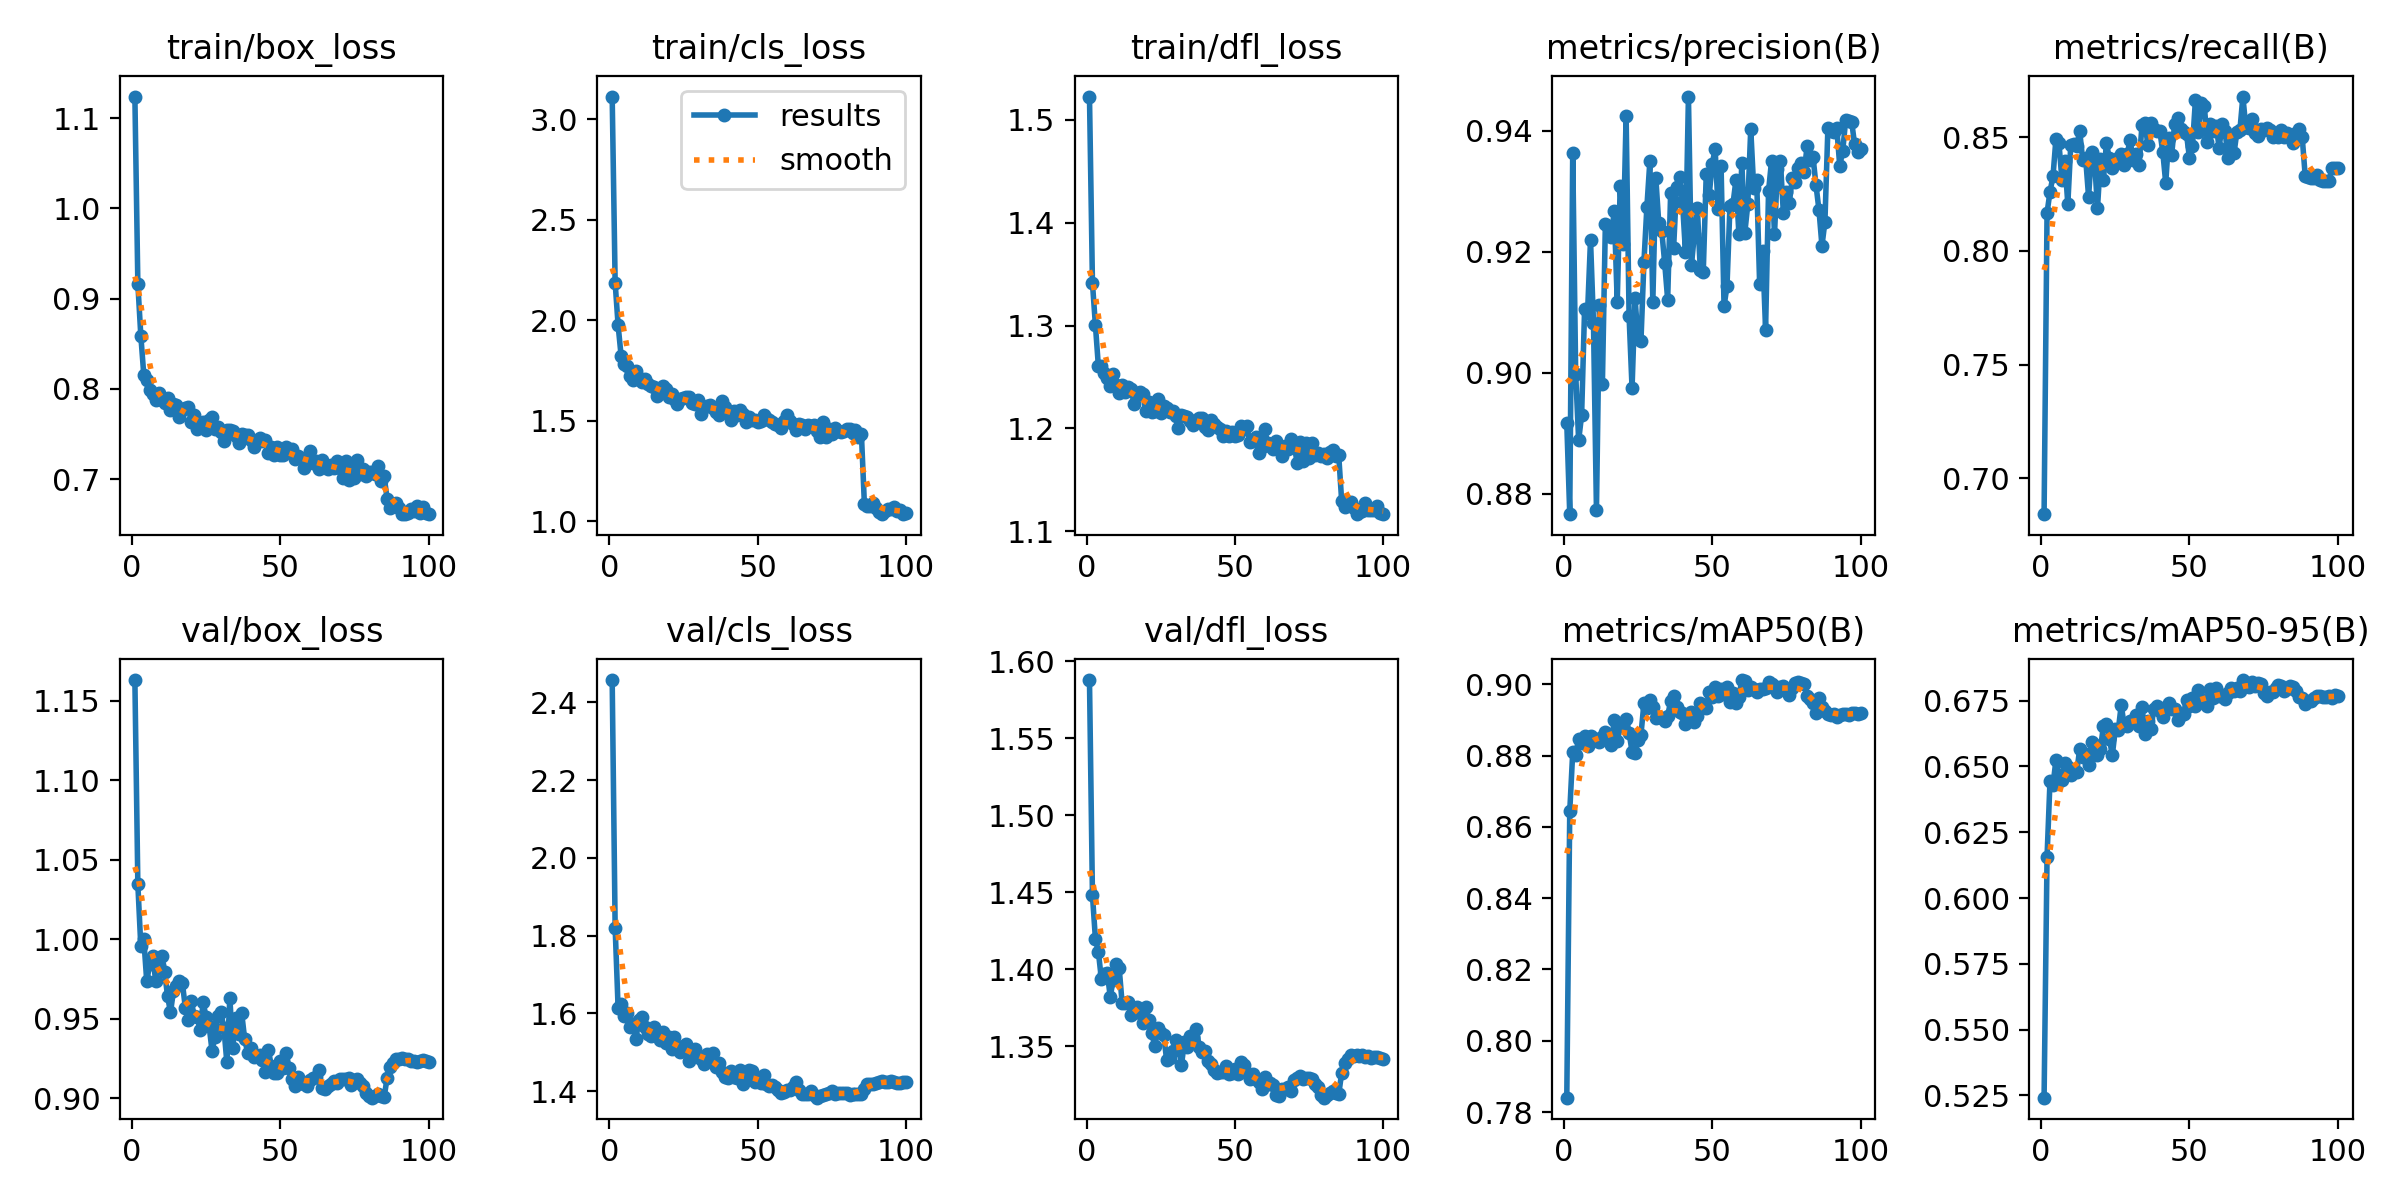
\includegraphics[width=\textwidth]{figures/images/results/y8x_phase2_12803/results.png}
    \caption{Tanítási és validációs veszteség-, valamint metrikagörbék a 100 epokon át}
    \label{fig:phase2_results}
\end{figure}

Az \ref{fig:phase2_results}. ábrán látható, hogy a tanítási és validációs veszteségek (\textit{box loss}, \textit{cls loss},
\textit{dfl loss}) mindhárom esetben folyamatosan csökkentek a tanítás során. A \textit{box loss} az első epokban $1{,}12$-ről
indult, és $0{,}66$ körüli értékre stabilizálódott, jelezve, hogy a modell egyre pontosabban jelöli ki a hibaterületeket.
A \textit{cls loss} meredekebb esést mutatott az első 10 epokban ($3{,}11 \rightarrow 1{,}71$), majd fokozatosan $1{,}04$
közelébe konvergált, ami az osztályozás gyors és megbízható javulására utal.

A validációs mAP50 metrika az 1. epokban $0{,}784$-ről indult, és a 60. epokban érte el csúcsértékét: $\mathbf{0{,}901}$.
A mAP50-95 értéke a 68. epokban tetőzött $\mathbf{0{,}683}$ értéken. A tanítás végére (100. epok) a modell
stabilan $0{,}892$ (mAP50) és $0{,}677$ (mAP50-95) körüli teljesítményt nyújtott. A koszinuszos tanulási ráta csökkentés
a 86. epokban okozott kisebb zökkenőt a veszteséggörbéken (a \textit{close mosaic} beállítás lezárása miatt), amelyet
a modell gyorsan kompenzált.

\subsection{Precision-Recall görbe}

\begin{figure}[H]
    \centering
    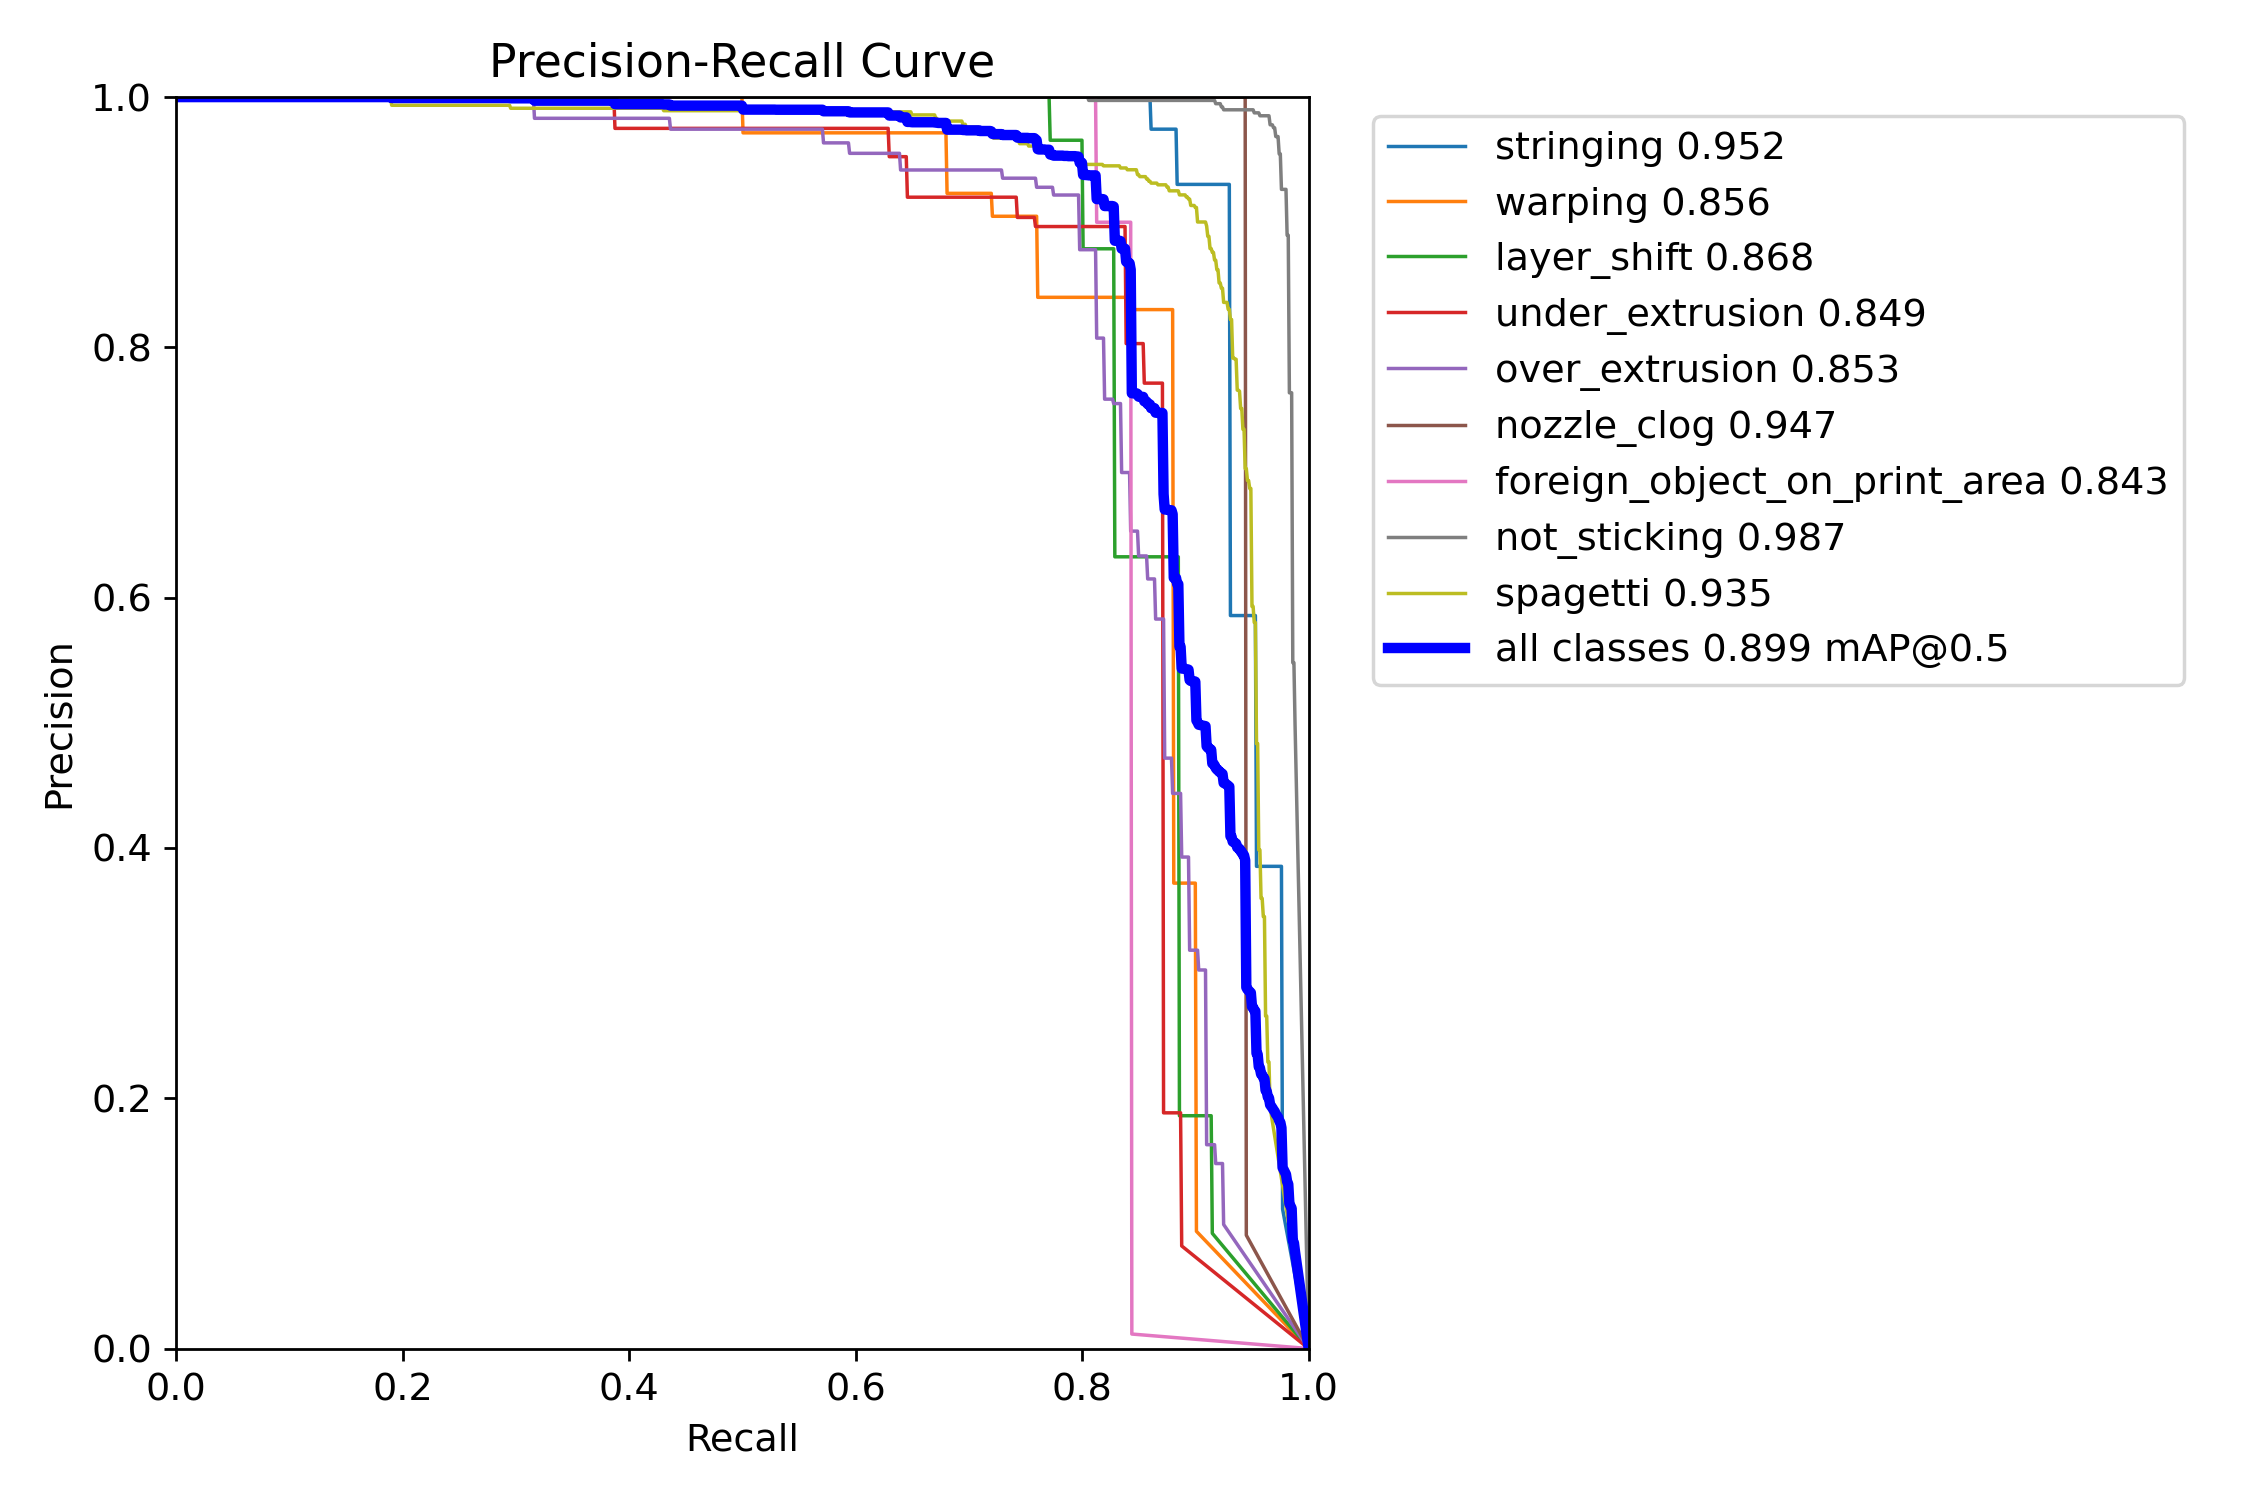
\includegraphics[width=0.8\textwidth]{figures/images/results/y8x_phase2_12803/BoxPR_curve.png}
    \caption{Precision-Recall görbe osztályonként (\texttt{y8x\_phase2\_12803})}
    \label{fig:phase2_pr}
\end{figure}

A \ref{fig:phase2_pr}. ábra az egyes hibaosztályok Precision-Recall görbéit mutatja. Az összes osztályra vonatkozó
összesített mAP@0.5 értéke $\mathbf{0{,}892}$. A görbék alapján megállapítható, hogy a modell a legtöbb hibaosztályt
magas pontossággal képes felismerni. A kisebb területű vagy vizuálisan hasonló hibatípusok, például az
\textit{under\_extrusion} és a \textit{nozzle\_clog}, esetén a görbe alatti terület alacsonyabb, ami ezeknek az
osztályoknak a nagyobb detekciós nehézségét tükrözi.

\subsection{F1-konfidencia görbe}

\begin{figure}[H]
    \centering
    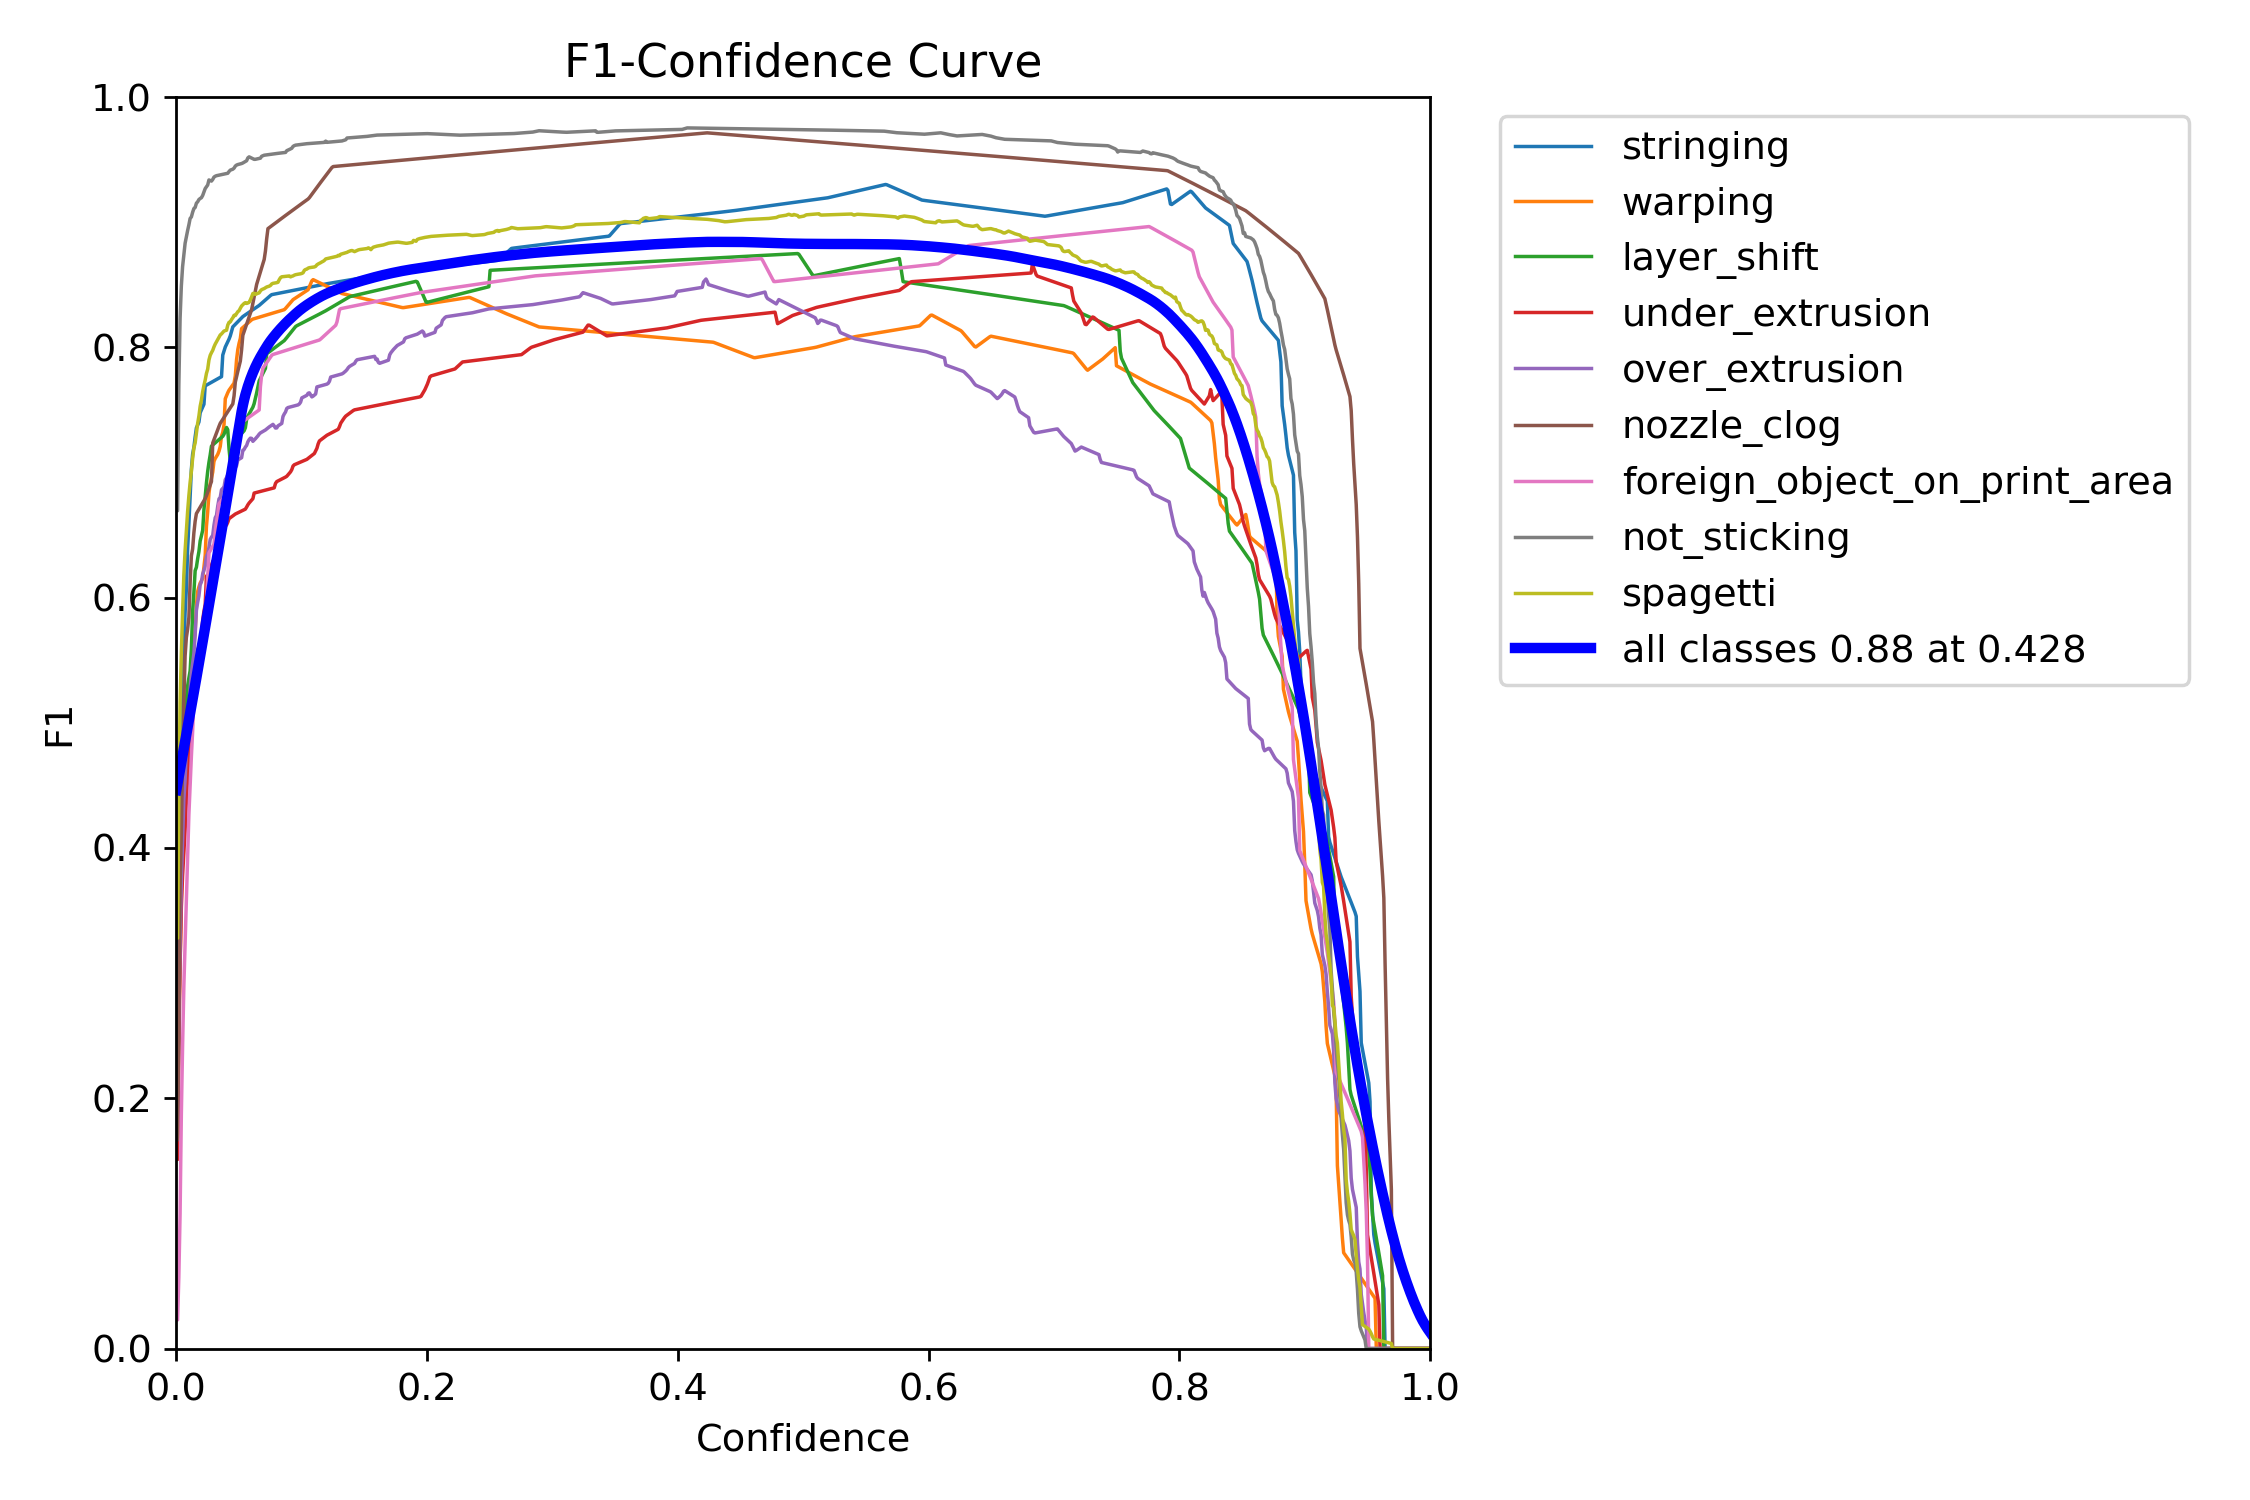
\includegraphics[width=0.8\textwidth]{figures/images/results/y8x_phase2_12803/BoxF1_curve.png}
    \caption{F1-konfidencia görbe osztályonként (\texttt{y8x\_phase2\_12803})}
    \label{fig:phase2_f1}
\end{figure}

Az \ref{fig:phase2_f1}. ábra az F1-pontszámot ábrázolja a konfidenciaküszöb függvényében. A csúcs-F1 értéke
$\mathbf{0{,}88}$, amelyet $\approx 0{,}38$ körüli konfidenciaküszöbnél ér el a modell. Ez azt jelenti, hogy a
precizitás és a visszahívási arány optimális egyensúlya ennél a küszöbértéknél érhető el az éles alkalmazásban.
A görbe viszonylag lapos a $0{,}2$-$0{,}55$ tartományban, ami robusztus viselkedésre utal a konfidenciaküszöb
finomhangolásával szemben.

\subsection{Konfúziós mátrix}

\begin{figure}[H]
    \centering
    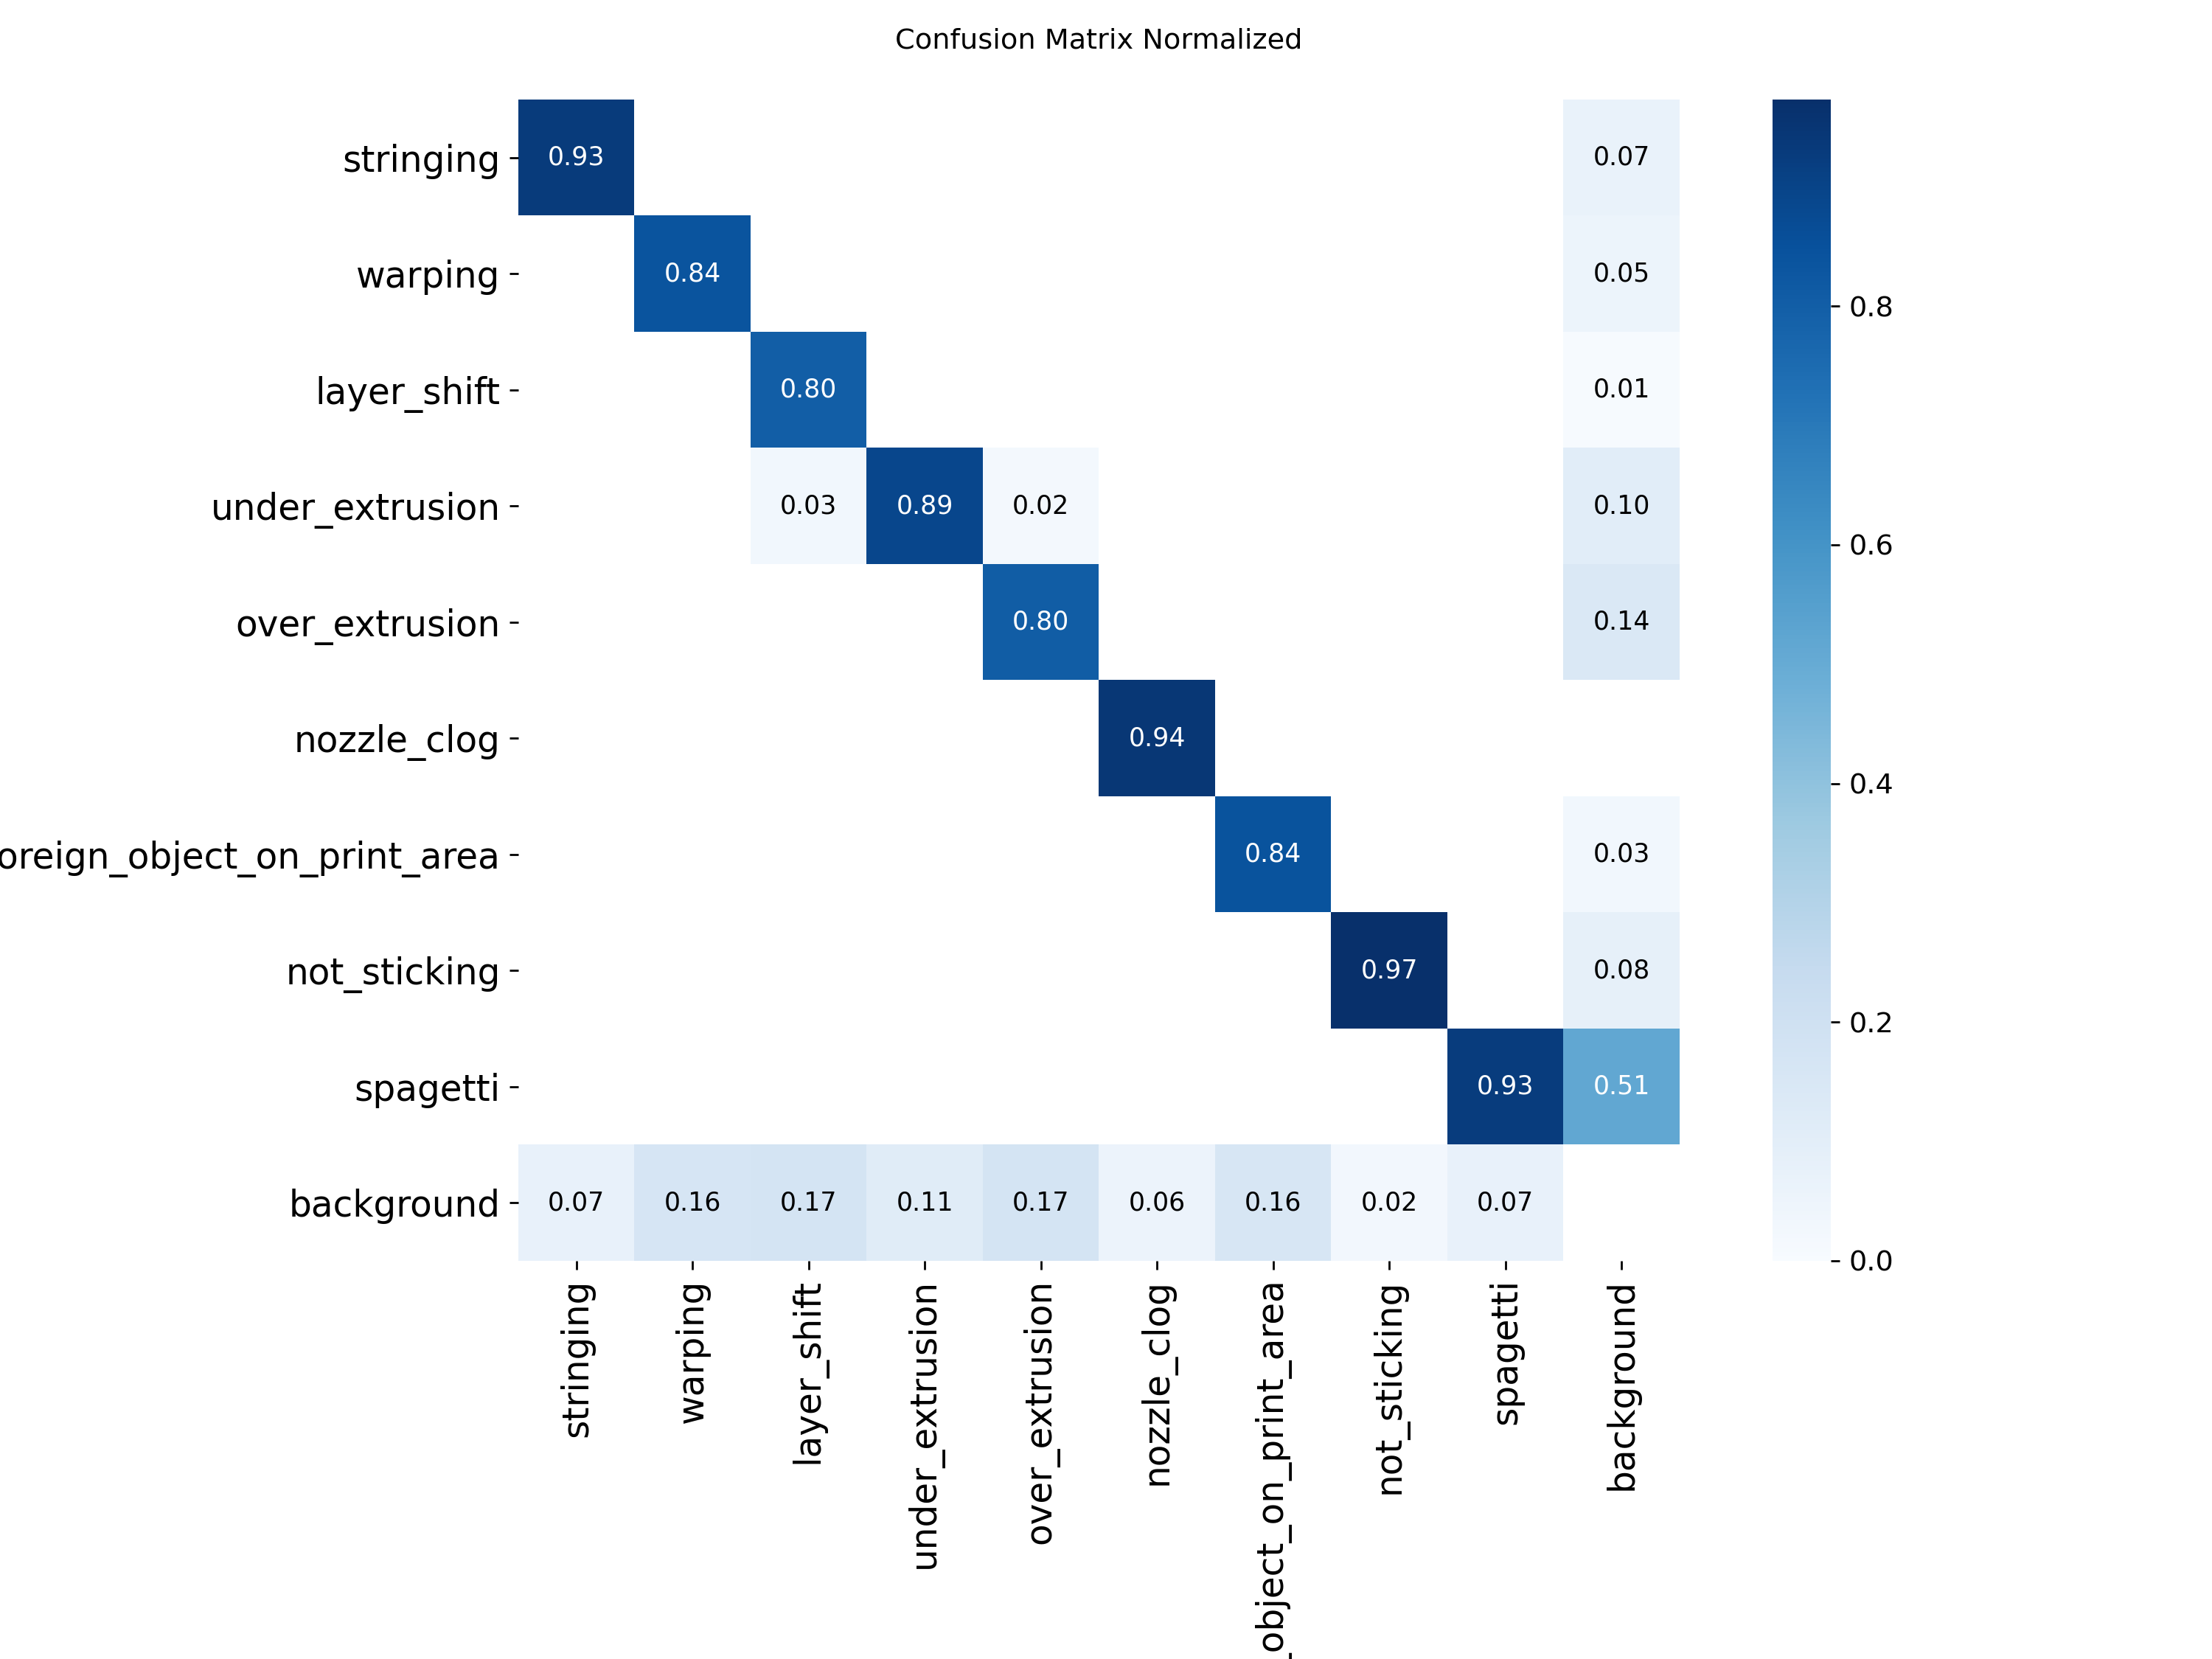
\includegraphics[width=\textwidth]{figures/images/results/y8x_phase2_12803/confusion_matrix_normalized.png}
    \caption{Normalizált konfúziós mátrix (\texttt{y8x\_phase2\_12803})}
    \label{fig:phase2_cm}
\end{figure}

A \ref{fig:phase2_cm}. ábra normalizált konfúziós mátrixa az egyes osztályok közötti tévesztések arányát mutatja.
Az átló mentén látható értékek a helyes detekciók arányát jelölik osztályonként. A mátrix alapján a modell a legtöbb
hibatípust megbízhatóan azonosítja, a \textit{background} (háttér) osztályba kerülő tévesztések főként a kisebb méretű
vagy ritkábban előforduló hibaobjektumoknál figyelhetők meg.

\subsection{Validációs predikciók}

\begin{figure}[H]
    \centering
    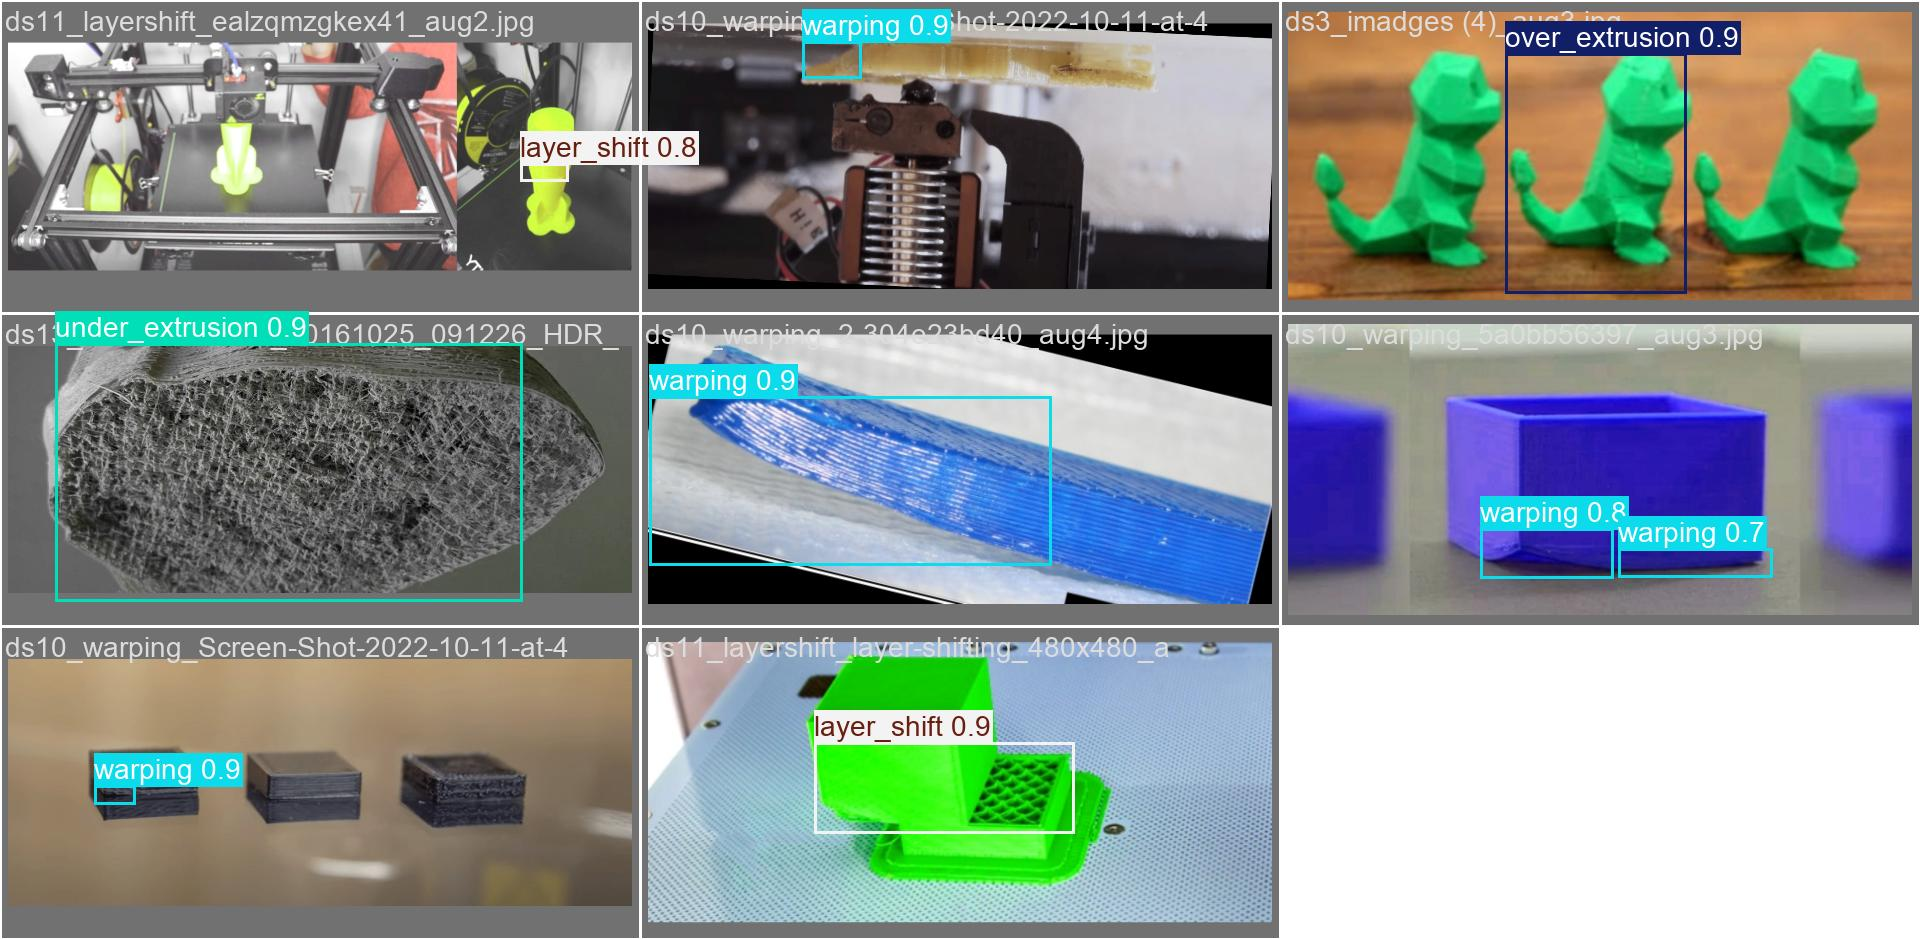
\includegraphics[width=\textwidth]{figures/images/results/y8x_phase2_12803/val_batch0_pred.jpg}
    \caption{Példa validációs batch modelljóslatok (\texttt{y8x\_phase2\_12803})}
    \label{fig:phase2_valpred}
\end{figure}

A \ref{fig:phase2_valpred}. ábra egy validációs batch modell által generált jelölődobozait mutatja. A vizuális
ellenőrzés megerősíti, hogy a modell pontosan lokalizálja és osztályozza a 3D nyomtatási hibákat, a határoló dobozok
jól illeszkednek a valós hibaterületekre.

\section{Összesített teljesítmény}

\begin{table}[H]
\centering
\caption{A \texttt{y8x\_phase2\_12803} modell végső teljesítménymutatói (100. epok)}
\label{tab:phase2_final}
\renewcommand{\arraystretch}{1.4}
\begin{tabular}{|l|c|}
    \hline
    \textbf{Metrika} & \textbf{Érték} \\
    \hline
    Pontosság (Precision) & $0{,}937$ \\
    \hline
    Visszahívás (Recall)  & $0{,}836$ \\
    \hline
    mAP@0.5               & $0{,}892$ \\
    \hline
    mAP@0.5:0.95          & $0{,}677$ \\
    \hline
    Legjobb mAP@0.5 (60. epok) & $\mathbf{0{,}901}$ \\
    \hline
    Legjobb mAP@0.5:0.95 (68. epok) & $\mathbf{0{,}683}$ \\
    \hline
\end{tabular}
\end{table}

A táblázatban összefoglalt eredmények alapján megállapítható, hogy a kétfázisú tanítási stratégia és a magas bemeneti
felbontás ($1280 \times 1280$ px) kombinációja hatékonyan javította a modell detekciós képességét. A $0{,}901$-es
csúcs-mAP@0.5 érték azt igazolja, hogy a modell megbízhatóan képes azonosítani a 3D nyomtatási hibákat valós
körülmények között is.


%\chapter{Tesztelés és kiértékelés}
%\input{chapters/test_and_validate.tex}

\chapter{Rendszerintegráció és alkalmazás}
\section{A rendszer életciklusa}

Az előző fejezetekben külön-külön kerültek bemutatásra az adatgyűjtés, a modell betanítása és az infrastruktúra egyes komponensei.
Ez a fejezet azt mutatja be, hogyan illeszkednek ezek a részek egy egységes, üzemelő rendszerré: mi a telepítés sorrendje,
hogyan indul el a pipeline, és hogyan kerül a betanított modell éles környezetbe.

\section{A betanított modell integrálása}

A betanítási folyamat végén keletkező \texttt{best.pt} súlyfájl a \texttt{judge} Docker konténerbe kerül becsomagolásra.
A konténer induláskor betölti ezt a fájlt, és az Ultralytics YOLOv8 API-ján keresztül elérhetővé teszi azt
a Vertex AI végpont HTTP interfészén. A modellcsere folyamata a következő lépésekből áll:

\begin{enumerate}
    \item Az új \texttt{best.pt} fájlt a \texttt{judge/} könyvtárba másoljuk.
    \item A \texttt{docker-judge.yml} GitHub Action workflow automatikusan lefut, újrabuildeli a \texttt{judge} image-t,
          és feltölti az Artifact Registry-be, a commit SHA-val mint egyedi taggel.
    \item A Vertex AI végpont a következő aktiváláskor az új image-t húzza le és futtatja.
\end{enumerate}

Ez a folyamat biztosítja, hogy a modell minden frissítése verziókövetett, visszagörgetható és automatizált legyen, kézi szerverhozzáférés nélkül.

\section{Telepítési sorrend}

Az első telepítés során a következő sorrendben kell elvégezni a lépéseket:

\subsection{Cloud infrastruktúra provisioning}

Az infrastruktúra felállítása Terraform segítségével történik. A \texttt{terraform apply} parancs kiadása után
automatikusan létrejönnek a Pub/Sub topicok, a Cloud Functions, a Vertex AI végpont, a Firestore kollekciók
és az Artifact Registry repository. Az infrastruktúra változtatásai a \texttt{main} ágra való merge esetén
a CI/CD pipeline automatikusan alkalmazza, így a rendszer mindig a konfigurációval összhangban van.

\subsection{A \texttt{judge} konténer telepítése}

A \texttt{judge} Docker image buildelése és Artifact Registry-be való feltöltése szintén automatizált:
a \texttt{docker-judge.yml} GitHub Action lefuttatja a buildet és a push eseményt, amelyet a Vertex AI végpont
az első hívásakor automatikusan lehív. A konténer telepítéséhez nincs szükség manuális Docker parancsokra.

\subsection{Az edge eszköz beállítása}

A Raspberry Pi-n az alábbi három systemd szolgáltatást kell egyszeri konfigurációval engedélyezni:

\begin{itemize}
    \item \textbf{MediaMTX} - a kamerastream RTSP publikálásáért felelős.
    \item \textbf{frame-extractor} - a képkockák kinyeréséért és Pub/Sub-ra való publikálásáért felelős.
    \item \textbf{cloudflared} - a Cloudflare alagút fenntartásáért felelős, amelyen keresztül a dashboard eléri az RTSP streameket.
\end{itemize}

A szolgáltatások az eszköz bekapcsolásakor automatikusan elindulnak, emberi beavatkozás nélkül.
A \texttt{frame-extractor} konfigurációja (RTSP URL-ek, GCP projekt azonosítója, topic neve) környezeti
változókon keresztül adható meg, így ugyanaz a konténer különböző nyomtatóállomásokon is újrafelhasználható.

Mivel a képkockák időbélyege a rögzítés pillanatában keletkezik, és a felhő oldalán a Dispatcher az ennél elavultabb
képkockákat eldobja, a Pi órájának pontosnak kell lennie; ehhez az eszközön futnia kell egy idő-szinkronizáló
szolgáltatásnak (például \texttt{systemd-timesyncd} vagy NTP).

\section{Az üzemelési folyamat}

Miután a rendszer telepítve és elindítva van, a következő folyamat zajlik le automatikusan,
emberi beavatkozás nélkül (lásd \ref{fig:systemarch}. ábra):

\begin{enumerate}
    \item A Raspberry Pi-n futó \texttt{frame-extractor} szolgáltatás a három RTSP streamből
          \textbf{kameránként tíz másodpercenként egy képkockát} dolgoz fel (alapértelmezetten 0,1 fps), átméretezi és JPEG-be tömöríti azokat,
          majd JSON üzenetként publikálja a \texttt{frames-in} Pub/Sub topicra.

    \item A \textbf{Dispatcher} Cloud Function feliratkozik a \texttt{frames-in} topicra.
          Minden beérkező üzenetnél a base64-kódolt képkockát a Vertex AI végpont \texttt{/predict} végpontjára
          továbbítja OAuth2 hitelesítéssel.

    \item A \textbf{Vertex AI végponton} futó \texttt{judge} konténer elvégzi az objektumdetekciót
          a YOLOv8 modell segítségével. A téves riasztások szűrésére csak azokat a hibákat tekinti megerősítettnek, amelyek
          legalább három egymást követő képkockán át láthatók ugyanazon a kamerán. Az eredményt, a detektált hibaosztályokat,
          konfidenciaértékeket és határoló téglalapokat, minden képkockára visszapublikálja a \texttt{detections-out} topicra.

    \item Az \textbf{Alert-Manager} Cloud Function feldolgozza a detekciós eredményeket. Minden beérkező inferenciát
          naplóz a Firestore \texttt{inferences} kollekciójába, a 35\%-os konfidenciaküszöböt elérő detektálásokat pedig
          az \texttt{alerts} kollekcióba is beírja. Magas prioritású hibák (\texttt{spagetti}, \texttt{not\_sticking}, \texttt{layer\_shift}, \texttt{warping})
          esetén HTML e-mail értesítést küld a kezelőnek, egyetlen, az egész rendszerre közös 300 másodperces cooldown alkalmazásával.

    \item A \textbf{dashboard} a Firestore \texttt{onSnapshot} listenerén keresztül valós időben jeleníti meg
          az újonnan érkező riasztásokat, egyidejűleg pedig a Cloudflare alagúton keresztül élőben mutatja
          a három kamera videofolyamát.
\end{enumerate}

\section{A dashboard használata}

A webes felület megnyitása után az operátor két nézetből felügyeli a teljes nyomtatási folyamatot:

\begin{itemize}
    \item \textbf{Live streams} - a három kamera élő WebRTC videofolyamát jeleníti meg egymás mellett, a nemrég megerősített
          detekciók jelöléseivel együtt. Ezen a nézeten található a rögzítés be- és kikapcsolására szolgáló vezérlő is,
          amely csak operátori Google-fiókkal bejelentkezve használható.
    \item \textbf{Inference log} - a feldolgozott képkockák naplója: minden bejegyzéshez megjeleníti a képkocka-bélyeget és
          a hozzá tartozó detekciók táblázatát (hibaosztály, konfidenciaérték, kamera azonosítója, időbélyeg), a határoló téglalapokat
          pedig pontosan a feldolgozott képkockára rajzolva.
    \item \textbf{Állapotjelzés} - magas prioritású hiba esetén a felület piros kerettel jelez (\textit{alerting}
          állapot); költségvetési küszöb átlépésekor sárga kerettel (\textit{budget-alert} állapot).
\end{itemize}

\section{Konfigurálhatóság és skálázhatóság}

A rendszer tervezésekor fontos szempont volt, hogy könnyen adaptálható legyen különböző üzemelési körülményekhez.

\subsection{Konfidenciaküszöb}

Az Alert-Managerben beállított 35\%-os konfidenciaküszöb az alkalmazás environment változóján keresztül módosítható.
Magasabb küszöb kevesebb, de megbízhatóbb riasztást eredményez; alacsonyabb küszöb érzékenyebb, de több fals pozitívot
is hozhat. Az optimális érték meghatározása a jövőbeli tesztelési terv részeként valósul majd meg (lásd Összefoglalás és jövőbeli irányok fejezet).

\subsection{Képkockaráta és felbontás}

A \texttt{frame-extractor} \texttt{CAPTURE\_FPS} és \texttt{FRAME\_WIDTH}/\texttt{FRAME\_HEIGHT} paraméterei
lehetővé teszik a valós idejű terhelés és a Pub/Sub átviteli kapacitás közötti egyensúly megtalálását.
Gyorsabb nyomtatóknál magasabb fps értékkel érdemes dolgozni; hálózati sávszélesség korlát esetén
az alacsonyabb JPEG minőség csökkenti az átviteli méretet.

\subsection{Több nyomtatóállomás}

Az architektúra horizontálisan skálázható: további Raspberry Pi egységek és kamerakészletek az egyedi
\texttt{CAMERA\_IDS} és \texttt{RTSP\_URLS} értékek megadásával csatlakoztathatók a meglévő pipeline-hoz,
anélkül, hogy a cloud komponenseket módosítani kellene. A Pub/Sub és a Cloud Functions automatikusan skálázódnak
a megnövekedett üzenetterheléssel.

\subsection{Modellcsere}

Mivel a detekciós modell a \texttt{judge} konténertől elkülönítve, a \texttt{best.pt} fájl cseréjével frissíthető,
egy jobb modell telepítése nem igényli a teljes infrastruktúra újraépítését. Elegendő az új súlyfájlt
a \texttt{judge/} könyvtárba helyezni és a GitHub Action workflow-t lefuttatni.

\section{Ismert korlátok}

A jelenlegi implementáció az alábbi korlátokat mutatja:

\begin{itemize}
    \item A képkockákat tároló GCS bucket nyilvánosan olvasható, és nincs hozzá élettartam-szabály (\textit{lifecycle rule}),
          így a feltöltött képek korlátlanul gyűlnek. Éles üzemeltetéshez automatikus törlési szabály és szűkebb hozzáférés indokolt.
    \item Nincs külön életjel-figyelés (\textit{heartbeat}) a Raspberry Pi-re: ha a \texttt{frame-extractor} leáll, a \texttt{frames-in}
          csatorna elcsendesedik, de erről a rendszer nem küld riasztást, csak a dashboard csempéi sötétednek el.
    \item A Vertex AI végpont aktív használaton kívül is fenntart egy minimális példányt, amely napi
          $\approx$37 USD folyamatos üzemelési költséggel jár. Alacsony intenzitású monitorozáshoz
          a \textit{scale-to-zero} beállítás alkalmazása csökkentheti a kiadásokat, de növeli a hideginduló
          késleltetést (\textit{cold start}).
    \item A jelenlegi konfidenciaküszöb (35\%) empirikusan lett beállítva; a valós nyomtatási körülmények
          között végzett mérések alapján ezt finomhangolni szükséges (lásd Összefoglalás és jövőbeli irányok fejezet).
\end{itemize}


\chapter{Összefoglalás és jövőbeli irányok}
\section{Összefoglalás}

A jelen dolgozat egy valós idejű, mesterséges intelligencián alapuló 3D nyomtatási hibadetektor rendszer
tervezését és megvalósítását mutatta be, amelynek célja az FDM technológiával üzemelő nyomtatófarmok
automatizált felügyelete.

A munka első szakaszában az iparági igények és a kapcsolódó szakirodalom elemzésével meghatároztuk azokat
a leggyakoribb és gazdaságilag legjelentősebb hibatípusokat -- spagetti, nem tapadó réteg, réteg-eltolódás,
vetemedés, szálazás, alul- és felülextrúdálás, fúvóka-dugulás, idegen tárgy --, amelyek automatikus
detektálása a legtöbb értéket hozza a nyomtatógazdálkodásban.

Az adatgyűjtési fázisban három nyilvánosan elérhető adathalmaz, automatizált webes képletöltés és 397 saját
készítésű felvétel kombinációjából \textbf{2422 annotált képből} álló adathalmazt állítottunk össze.
Az annotálás CVAT eszközzel, kilenc osztályra, bounding-box formátumban történt. Az osztályegyensúly-hiányt
oversampling technikával, a vizuális diverzitást pedig egy háromrétegű augmentációs pipeline-nal --
alaptranszformációk, Smart MixUp és mozaik -- korrigáltuk, amelynek eredményeként a tanítókészlet közel
négyszeresére bővült.

A modellezési szakaszban a YOLOv8x architektúrát alkalmaztuk, kétfázisú tanítási stratégiával.
Az első fázis 960 képpontos bemeneti felbontáson általánosabb jellemzők megtanulását célozta, míg a
második fázis 1280 képpontos felbontáson, az első fázis legjobb súlyaiból kiindulva, finomhangolással
tovább javított a részletgazdag hibaminták felismerésén. A betanított modell végső teljesítménymutatói:

\begin{table}[H]
\centering
\caption{A betanított YOLOv8x modell összesített teljesítménye}
\renewcommand{\arraystretch}{1.4}
\begin{tabular}{|l|c|}
    \hline
    \textbf{Metrika} & \textbf{Érték} \\
    \hline
    Pontosság (Precision) & $0{,}937$ \\
    \hline
    Visszahívás (Recall)  & $0{,}836$ \\
    \hline
    mAP@0.5               & $0{,}892$ \\
    \hline
    mAP@0.5:0.95          & $0{,}677$ \\
    \hline
    Csúcs mAP@0.5         & $0{,}901$ \\
    \hline
    Csúcs F1              & $0{,}88$ \\
    \hline
\end{tabular}
\end{table}

A rendszerintegrációs szakaszban egy edge--cloud hibrid architektúra valósult meg. A helyszíni komponenst
egy Raspberry Pi 4B adja, amelyen három webkamera képkockáit egy \texttt{frame-extractor} szolgáltatás
gyűjti és publikálja Google Cloud Pub/Sub csatornára. A felhőoldali pipeline egy Dispatcher Cloud Function,
egy Vertex AI-n futó \texttt{judge} konténer (YOLOv8 inferenciával), egy Alert-Manager Cloud Function,
valamint egy Firestore-alapú valós idejű webes dashboard elemeiből épül fel. Az infrastruktúra
Terraformmal kezelt, a modellfrissítések CI/CD workflow-n keresztül történnek -- emberi beavatkozás nélkül.

A rendszer három kameraállásból, másodpercenként hat képkockát dolgoz fel, és magas prioritású hiba
észlelésekor e-mail értesítést küld a kezelőnek, 60 másodperces kameránkénti cooldown-nal a riasztásözön
elkerülése érdekében.

% -------------------------------------------------------------------
\section{Jövőbeli irányok}

A jelenlegi megvalósítás több ponton is tovább fejleszthető:

\begin{itemize}
    \item \textbf{Konfidenciaküszöb finomhangolása.} A jelenlegi 35\%-os küszöb empirikusan lett
    meghatározva. Éles nyomtatási körülmények között szisztematikus mérésekkel -- precision--recall
    kompromisszum elemzéssel -- pontosabb, üzemspecifikus érték határozható meg.

    \item \textbf{Állandó Cloudflare alagút.} Az ideiglenes \textit{quick tunnel} minden Pi-újraindításkor
    új URL-t kap, ami megszakítja a dashboard stream-kapcsolatát. Éles üzemeltetéshez \textit{named tunnel}
    konfigurációra van szükség.

    \item \textbf{Vertex AI scale-to-zero.} A végpont jelenlegi minimálpéldánya napi $\approx$37 USD
    üzemelési költséggel jár. Alacsony intenzitású monitorozási forgatókönyvekben a \textit{scale-to-zero}
    beállítás jelentős megtakarítást hozhat a hideginduló késleltetés elfogadható növelése árán.

    \item \textbf{Bővített osztálykészlet.} Az adathalmaz elsősorban az FDM technológia legelterjedtebb
    hibatípusait fedi le. Speciálisabb hibák -- például fúvóka-kopás, rétegleválás, hőmérsékleti
    anomáliák -- bevonásával a rendszer alkalmazhatósági köre bővíthető.

    \item \textbf{Modell könnyűsúlyúsítása.} A YOLOv8x nagy kapacitású modell; edge eszközön történő
    futtatáshoz YOLOv8n vagy YOLOv8s változatra való átállás, illetve kvantálás csökkenthetné
    a felhőinfrastruktúra igénybevételét és a késleltetést.

    \item \textbf{Aktív tanulás.} A rendszer üzemelés közben gyűjti a valós nyomtatási képeket.
    Egy aktív tanulási ciklus bevezetésével az operátor által megerősített vagy korrigált detekciók
    visszacsatolhatók az adathalmazba, folyamatosan javítva a modell teljesítményét.

    \item \textbf{Nyomtatóvezérlő integráció.} Jelenleg a rendszer csak értesít; a következő lépés
    a detektált hiba súlyosságától függő automatikus beavatkozás -- például a nyomtatás szüneteltetése
    vagy leállítása -- megvalósítása lenne OctoPrint vagy Klipper API-n keresztül.
\end{itemize}


%\chapter{Mellékletek}
%\input{chapters/melleklete.tex}

% ════════════════════════════════════════════════════════════════════════════
% BIBLIOGRAPHY  (bibtex / ieeetr — matches CI compileLatex.yml)
% ════════════════════════════════════════════════════════════════════════════
\addcontentsline{toc}{chapter}{Irodalomjegyzék}
\bibliographystyle{ieeetr}
\bibliography{References}

%appendix
%\appendix
%\chapter{Függelék}
%\input{chapters/appendix}

\end{document}
